\chapter{Multi-version Execution}
\label{chap:multi-version}

\section{N-version \vs multi-version execution}

\section{Two applications of multi-version execution}
\subsection{Fail recovery for updated software}
\subsection{Parallel execution of software versions}
%\section{Prototype}
\label{sec:mx}

%% \begin{figure}[t!]
%% \centering
%% \includegraphics[width=\columnwidth]{safe-updates/figures/overview}
%% \caption{A platform running both conventional and multi-version
%%   applications.}
%% \label{fig:mx-platform}
%% \end{figure}

We have implemented our approach in a prototype system called \mx,
targeted at multi-core processors running Linux.  Currently, \mx
supports two versions run in parallel. The system works directly on
application binaries, making it easy to deploy it and possibly integrate
it with existing software package managers such as \texttt{apt} or
\texttt{yum}.

%Figure~\ref{fig:mx-platform} shows a platform running \mx, on which
On a platform using \mx, conventional (\ie unmodified) applications
and multi-version (\mv) applications run side by side.  The key
property that must hold on such a platform is that without purposely
trying to do so, applications should not be able to distinguish
between conventional and \mv applications running on the platform. In
particular, the multiple versions of an \mv application should appear
as one to any other entity interacting with them (\eg user, operating
system, other machines).  Furthermore, \mv applications should be more
reliable and secure than their component versions, and their
performance should not be significantly degraded.

To achieve these goals, our prototype \mx employs several different
components, as shown in the architectural overview of
Figure~\ref{fig:design}.  The input to \mx consists of the binaries of
two versions of an application, which we will refer to as 
\textit{the old version}---the one already running on the system, and 
\textit{the new version}---the one newly released.


These two binaries are first statically analysed by the \sea (Static
Executable Analyser) component, which constructs a mapping from the
control flow graph (CFG) of the old version to the CFG of the new
version (\S\ref{sec:sea}).  The two versions are then passed to \mxm
(Multi-eXecution Monitor), whose job is to run the two versions in
parallel, synchronise their execution, virtualise their interaction
with the outside environment, and detect any divergences in their
external behaviour (\S\ref{sec:mxm}).  Once a divergence is detected,
it is resolved by \rem (Runtime Execution Manipulator), which selects
between the available behaviours, and resynchronises the two versions
after the divergence (\S\ref{sec:rem}).

The system prototype has been implemented in C with a small amount of
assembly, and the current version has approximately \mxSLOC source
lines of code. The implementation currently supports Linux kernels
3.2.0 and above, running x86 and x86-64 architectures.

The rest of this section describes the main \mx system components and
their implementation in more detail, and discusses how they work
together to support safe software updates.

\begin{figure}[t!]
\begin{center}
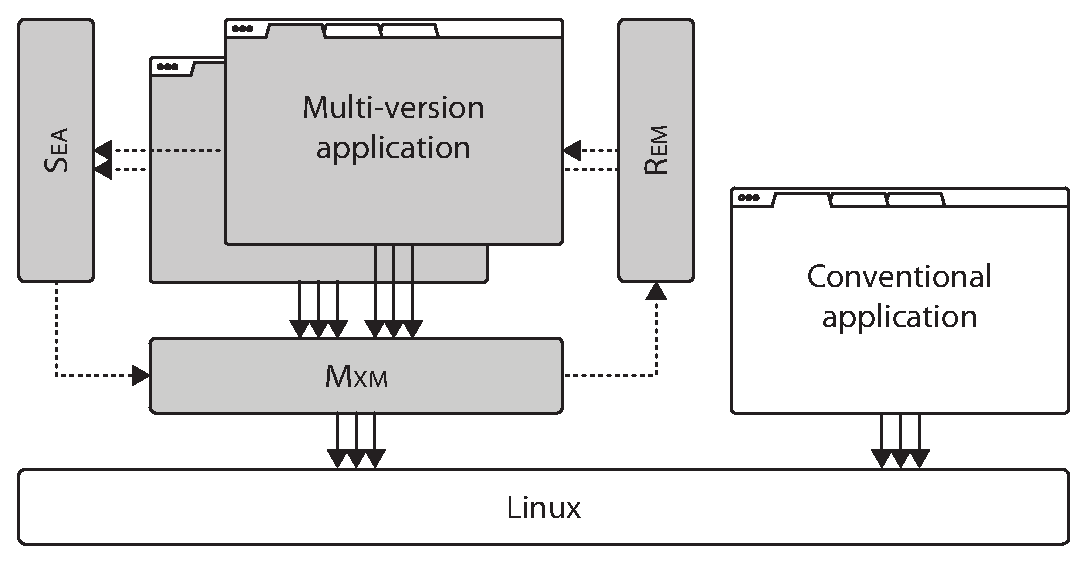
\includegraphics[width=0.6\columnwidth]{safe-updates/figures/architecture}
\caption{\mx system architecture.  
%% The main components of \mx
%%   are \sea (Static Executable Analyser), \mxm (Multi-eXecution
%%   Monitor), and \rem (Runtime Execution Manipulator).
}
\label{fig:design}
\end{center}
\end{figure}


\subsection{System call interposition}
\label{sec:mxm}

One of the main components of our multi-version execution environment
is the \mxm monitor.  \mxm's main jobs are to run the two versions
concurrently, mediate their interaction with the outside world,
synchronise their executions, and detect any divergences in their
external behaviour. \mxm works by intercepting all system calls issued
by each application version, and manipulating them to ensure that the
two versions are executed in a synchronised fashion and act as one to
the outside world.

\mxm provides functionality similar to conventional virtual machine monitors.
Whenever the MV application is executed, the \mxm connects to the two
application versions running in parallel, intercepting their kernel system
calls.  \mxm ensures that the two versions act as one to the outside world by
mediating access to the underlying operating system to achieve complete
isolation of the running application from other application instances as well
as from the external environment, making sure the combined application versions
act as one to the outside world.  The environment controlled by the monitor
consists mainly of a restricted file system access, socket interceptors and
signal handlers.

\subsubsection{System call interception}

\mxm is implemented using the  \ptrace interface provided by the Linux
kernel.  This interface, often used for application debugging, allows
simple deployment (without any need for compile-time instrumentation)
and makes the monitor itself lightweight since it is running as a
regular unprivileged process.  \mxm is similar in operation to previous
monitors whose goal is to synchronise applications at the level of system
calls such as \orchestra~\cite{orchestra09}, PLR~\cite{shye2009} or
\tachyon~\cite{tachyon12}.

\mxm runs each version in a separate child process, intercepting all
their system calls.  When a system call is intercepted in one version,
\mxm waits until the other version also performs a system call.  With
a pair of system calls in hand (one executed by the old version, and
one by the new version), \mxm compares their types and arguments.  If
they differ, \mxm has detected a divergence and invokes the \rem
component to resolve it (\S\ref{sec:rem}).

Otherwise, if the two versions perform the same system call with the
same arguments, \mxm virtualises their interaction with the
environment.  If the operation performed by the system call has no
side effects and does not involve virtualised state (\eg
\lstinline`sysinfo`), \mxm allows both processes to execute it
independently.  Otherwise, it executes the system call on their
behalf and copies its results into the address spaces of both
versions.

\mxm must also enforce deterministic execution across versions. This
consists mainly of intercepting instructions that may produce
non-deterministic results, and returning the same result in both
versions.  Examples of such non-deterministic operations include
random number generators (\eg read calls to \lstinline`/dev/[u]random`),
date and time (\eg read calls to \lstinline`/etc/localtime`), and access
to files and network (\eg file descriptor consistency).  Note that
non-deterministic effects resulting from allocating memory objects at
different addresses in memory or randomly arranging memory areas via
address space layout randomisation (ASLR) do not pose any
problems: \mxm understands the semantics of individual system calls and
rather than directly comparing memory addresses (which might be
different in each executed version), it compares the actual values
stored at those memory locations. \mxm supports both memory buffers (by
comparing the actual buffer content) as well as data structures
referenced by pointers (including nested ones).
 
Since \mxm fully controls executing programs intercepting all their system
calls, it can ensure that both programs have the same view of their
environment. Whenever the monitored process makes a system call, \mxm is
notified twice---first before, then after the call has been executed.  When a
\ptrace event is raised (\eg a new child process has been started), the monitor
is notified as well.  Due to internal limitations of the \ptrace interface,
once the system call has been made, it cannot be skipped, so when \mxm wants to
execute the call on behalf of its child processes, it simply replaces it with a
system call that does not change the system state (\lstinline`getpid` in our
case).

There are several challenges that we encountered while implementing
\mxm.  First, \mxm must partly understand the semantics of 
system calls.  For example, many system call parameters use complex
(often nested) structures with complicated semantics to pass values to
the operating system kernel, as in the case of \lstinline`ioctl` or
\lstinline`futex`.  To be able to compare the parameters of
these system calls and copy back their results, \mxm needs to
understand the semantics of these structures.  However, there are only
a relatively small number of system calls in Linux, and once the support
for handling them is implemented, it can be reused across applications.
\mxm currently implements \syscallsImplemented system calls (out of the
\syscallsTotal provided by Linux x86-64 3.1.9), which was enough to
allow us to run \mx on our benchmarks
(\S\ref{sec:reliability-evaluation}).

Second, the arguments of a system call are often passed through pointers,
which are only valid in the application address space, which is not directly
available to \mxm.  Therefore, \mxm needs to copy the contents pointed to by
these structures to its own address space in order to perform their
comparison.  The \ptrace interface on x86-64 only allows to copy one quadword
per system call, which is very expensive. Previous approaches either used
various ad-hoc optimisations~\cite{orchestra09} such as named pipes or shared
memory with custom shellcode, or a modified kernel~\cite{tachyon12} to
overcome this limitation. Instead, \mxm uses \emph{cross memory attach}, a new
mechanism for fast interprocess communication which has been recently added to
the Linux kernel~\cite{crossmemoryattach}.  This mechanism provides two new
system calls---\lstinline`process_vm_readv` and
\lstinline`process_vm_writev`---which allows the tracer to directly access the
memory space of the tracee using an interface similar to the \lstinline`readv`
and \lstinline`writev` system calls without any additional overhead.

Third, because the structures passed as arguments to system calls often have
variable size, \mxm also needs a fast way to allocate and deallocate memory
for them in order to minimise the overall overhead imposed by our system.  For
this purpose, \mxm uses a region-based memory allocator~\cite{memory-pools},
namely the \textsf{obstack}
library,\footnote{\url{http://www.gnu.org/software/hello/manual/libc/Obstacks.html}}
which is part of the \gnu C Library.  Each monitored process has its own
region, which is used for allocating memory to store the copy of the process'
system call arguments

\subsubsection{Multi-process and multi-threaded applications}

Finally, a particular challenge arises in the context of multi-process and
multi-threaded applications.  Using a single monitor instance to intercept both
versions and their child processes (or threads) would eliminate any advantage
that these applications derive from using concurrency.  Therefore, \mxm uses a
new monitor thread for each set of child processes (or threads) spawned by the
application.  For instance, if the old and new versions each have a parent and
a child process, then \mxm will use two threads: one to monitor the parent
processes, and one to monitor the child processes in each version.

Due to limitations of the \ptrace interface (which was not designed to be used
in a multi-process or multi-threaded environment), handing the control of any
child processes being spawned by the application over to a new monitoring
thread is somewhat complicated.  In \mxm we adopt a solution similar to
Orchestra~\cite{orchestra09}.  When a new child process is spawned, we let the
parent monitoring thread to supervise its execution until the first system
call.  Then, we replace this system call with a \lstinline`pause` system call,
disconnect the parent monitor (which causes a \lstinline`SIGCONT` signal to be
sent to all new child processes), and spawn a new monitoring thread which
immediately reconnects to the new child process, restores its original system
call, and resumes its execution.

\mxm does not enforce deterministic execution across multiple versions of
multi-threaded programs (which may diverge if race conditions can lead
to different external behaviour across executions), although we could
overcome this limitation by adopting \varan's solution
(\S\ref{sec:threading}).

%% \mxm also performs a series of optimisations to decrease performance
%% overhead, such as allowing certain files with read-only permissions
%% to be opened directly by the process. 

\subsubsection{Environment virtualisation}

To improve I/O performance and decrease virtualisation overhead,
processes are allowed to open files with read-only permissions
directly, while files with write permissions are opened by the monitor
itself.  This imposes another problem as file descriptors assigned to
these files are not necessarily the same in each version (\eg due to
scheduling non-determinism). Therefore, \mxm needs to virtualise
these file descriptors.

Whenever the monitored process opens a file with read-only permissions, a
new virtual file descriptor is assigned to this file together with the
mapping to a real file descriptor for each version. This virtual file
descriptor is then sent to each version. When a system call is made
using this virtual file descriptor, \mxm replaces it with the real
file descriptor before executing the system call. The actual file
operation is then executed by the process itself avoiding any memory
copying by \mxm.

A similar approach is also used for virtualisation of process,
group, parent and child identifiers.  Whenever a process tries to obtain
the actual ID, \mxm replaces this with a virtual ID and keeps the
mapping between the real and the virtual ID. When a process invokes a
system call using this ID as an argument (\eg \lstinline`kill`), the
virtual ID is replaced with the actual ID before executing the system
call.

%% \paragraph{Para-virtualisation interface and binary translation.}
%% Furthermore, we plan to combine this API with a binary translation
%% approach~\cite{binary-translation}, that will allow to dynamically
%% replace certain system calls with more efficient \emph{monitor
%% call} instructions.  The binary translation could be also used to
%% dynamically replace code components that have been proved to be
%% safe and do not need to be replicated across multiple versions (\eg
%% using static verification during compilation, using traces of
%% previous execution, using runtime heuristics).


%% \paragraph{Future work}

%% The \texttt{ptrace} interface allows us to easily monitor the program
%% execution without any compile-time instrumentation.  The main downside
%% of this approach is a relatively high overhead.  This is especially
%% true for I/O intensive applications, as they require frequent
%% transfers of large portions of the application memory space to the
%% monitor process. This overhead could be eliminated by directly
%% accessing the process memory space.

%% The existing prototype implementation of \textsc{Mxm} already supports
%% simple scenarios. The main limitation of this implementation is the
%% strict ordering of system calls, which must be the same in each
%% monitored application version.  To be practically usable, future
%% versions of \textsc{Mxm} need to relax the requirement on strict
%% ordering to allow more complex scenarios. This is especially important
%% when executing different versions of the same application.

%% Most importantly, a straightforward comparison of system call traces
%% is usually not sufficient to identify divergences, since different
%% versions might use a slightly different sequence of kernel and library
%% calls to implement the same behaviour.  We plan to explore approaches
%% similar to those implemented by compiler optimisations, such as
%% \emph{peep-hole optimisation}~\cite{dragon-book}, and adapt them to
%% work on the level of kernel and library calls.


%% %% \paragraph{Hashing system call traces.}
%% %% To decrease the overhead of kernel and library call synchronisation, we aim to
%% %% enhance our system to hash the sequence of system call traces using fast hash
%% %% functions such as FNV-1 or FNV-1a.  This approach has a significant advantage
%% %% over straightforward comparison of call traces, especially in the case of
%% %% system calls with virtually unlimited parameter sizes such as \texttt{read} or
%% %% \texttt{write}~\cite{shye2009}.  Similar approach has been already used
%% %% in~\cite{shye2009}.

%% \paragraph{Libraries support and virtualisation.}
%% Since many applications today use functionality provided by shared
%% libraries, we aim to support intercepting calls to such libraries as
%% well. Moreover, as intercepted calls to shared libraries can be
%% executed only once, same as in the case of system call monitoring,
%% this may decrease the overall overhead of multi-version execution.

%% We also plan to provide our own implementation of the \texttt{libc}
%% library loaded using the \texttt{LD\_PRELOAD} mechanism.  This library
%% will communicate directly with the monitor process through shared
%% memory, decreasing the number of system calls that need to be directly
%% intercepted, and thus resulting in much better performance.  However,
%% since the \texttt{LD\_PRELOAD} mechanism can be overridden, we still
%% need to combine it with the \texttt{ptrace} monitoring facility to
%% achieve complete isolation with reasonable overhead.  This approach
%% can be extended to support other shared libraries as well, further
%% improving the overall performance of our approach.

\subsection{Runtime state manipulation}
\label{sec:rem}

At the core of our system lies the \rem component, which is invoked
by \mxm whenever a divergence is detected.  \rem has two main jobs:
(1)~to decide whether to resolve the divergence in favour of the old or
the new version; and (2)~to allow the other version to execute through
the divergence and resynchronise the execution of the two versions
after the divergence.
%% The first task by itself it's easy: we favour the new version, except
%% for when it crashes.
%% As discussed in \sref{sec:scope}, in this paper we restrict our
%% attention to surviving crash errors, so the first task is relatively
%% easy: if one of the two versions crashes, we use the output of the
%% other version; otherwise, we always favour the new version.  
%%
%% The second task is however more difficult, but essential to the
%% success of our approach, which relies on having both versions be alive
%% at all times, so that the overall application can survive any crash
%% bugs that happen in either the old or the new version (although of
%% course, not in both).
%%
As discussed in Section~\ref{multi-version:rationale}, in \mx we focus
our attention on surviving crash errors, so the key challenge is to
allow the crashing version to survive the crash.  This is essential to
the success of our approach, which relies on having both versions alive
at all times, so that the overall application can survive any crash bugs
that happen in either the old or the new version (although of course,
not in both at the same time).

We emphasise that we apply our approach only to crash errors (those
raising a \lstinline`SIGSEGV` signal), and not to other types of program
termination, such as \lstinline`abort`.  This is important from a
security perspective, because
%% many patches turn potential compromises into
%% run-time {\small{\texttt{abort}s}}, \eg using assertions for input
%% sanitisation.  For example, 
when a vulnerability is discovered, but a proper solution is not yet
known, developers often\footnote{For example, see the patch in \texttt{json-cpp}~\url{http://jsoncpp.svn.sourceforge.net/viewvc/jsoncpp/trunk/jsoncpp/include/json/assertions.h?r1=247&r2=246&pathrev=247}}
fail-stop the program rather than letting it continue and allowing
the attacker to compromise the system.
%
%% Such situations can be easily distinguished since failed assertions
%% result in program abortion (\ie
%% \textstt{SIGABRT} signal), while unintentional program crashes typically
%% result in abnormal termination (\ie \textstt{SIGSEGV} signal). 
%% Therefore, \rem only intercepts and handles crashes resulting
%%   in \textstt{SIGSEGV} signals.

Suppose that one of the versions has crashed between the execution of
system call $s_1$ and the execution of system call $s_2$.  Then, in
many common scenarios, the code executed between the two system calls
is responsible for the crash (\eg the old version crashes because it
doesn't incorporate a bug fix present in the new version, or the new
version crashes because its code was patched incorrectly).  Therefore,
our strategy is to do a form of \textit{runtime code patching}, in
which we use the code of the non-crashing version to execute over the
buggy code in the crashing version.

%% If the behaviour of the two versions is different, but they both
%% continue to execute, then we favour the behaviour of the new version and
%% wait for the two versions to reconverge.

%% There are many different ways to achieve this goal, such as the use of
%% a mechanism based on check-pointing and roll-back~\cite{qin2005};
%% however, these mechanisms cannot deal with persistent errors which are
%% common in the case of software updates.

%% Our solution is based upon the observation that errors in programs are
%% usually located at particular places (\ie specific instructions) in
%% the program's code.  Therefore, we can use the code of the other, and
%% \ie correct, version to execute over this critical point in program's
%% code. This approach may not work when memory layout of the two
%% versions differs, as the code of one version may fail to locate the
%% memory structures necessary for its execution in the memory of the
%% other version. Nevertheless, the described approach might still work
%% in many cases when memory layout of the two versions does not differ
%% significantly.


%\paragraph{Possible execution scenarios.}

%% We run two versions of the same application in parallel, monitoring
%% their execution to be sure that they behave in the same way without
%% any divergences by comparing the application executions at
%% synchronisation points; in case of our prototype equal to system
%% calls. When either of the versions fail, we stop its execution at the
%% \emph{divergence point}; at this point there are three possible
%% solutions to synchronise the divergent versions:

\begin{figure}[t]
\centering
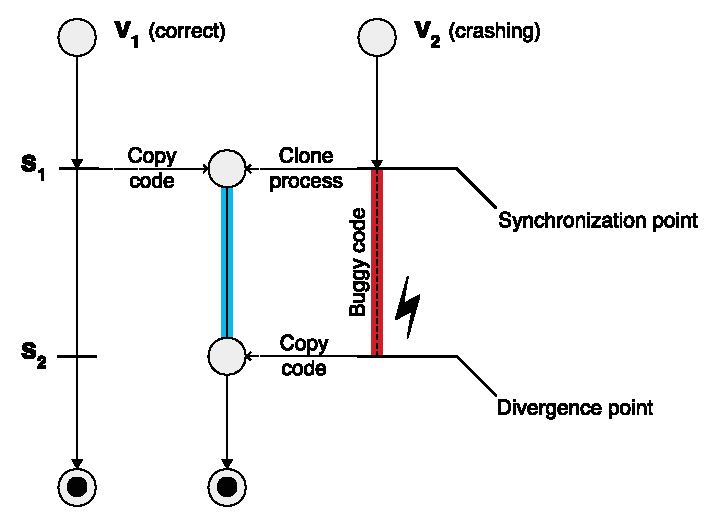
\includegraphics[width=0.5\columnwidth]{safe-updates/figures/strategy}
\caption{\rem's recovery mechanism uses the code of the non-crashing
  version to run through the buggy code.}
\label{fig:solution3}
\end{figure}

%% \begin{enumerate}[label=\emph{S\arabic*}, itemsep=3pt, parsep=3pt]
%% \renewcommand*\labelitemi{\emph{S\arabic*}}
%% \begin{figure}[t]
%%   \centering
%%   \subfloat[Patch state after the crash and continue execution]{
%%     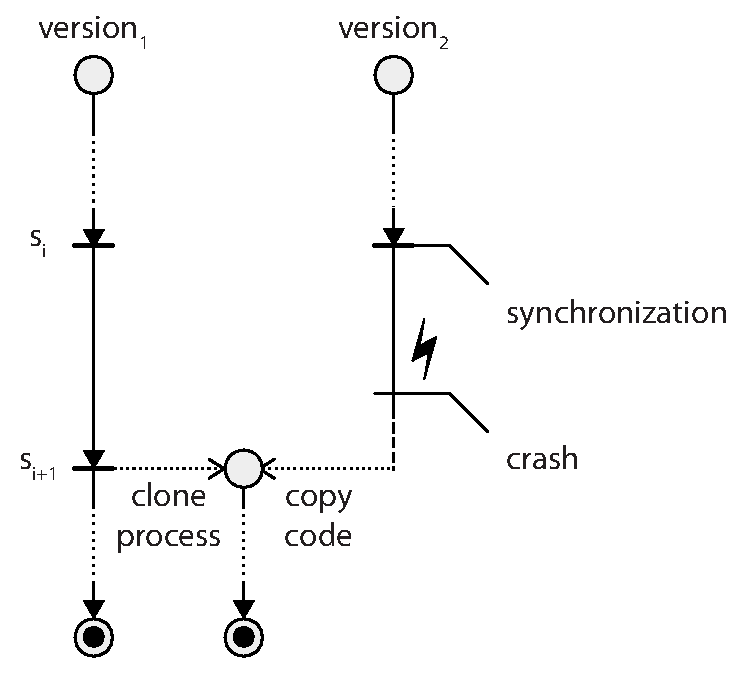
\includegraphics[width=0.45\columnwidth]{safe-updates/figures/solution1}
%%     \label{fig:solution1}
%%   }
%%   \quad
%%   \subfloat[Patch state before the crash and continue execution]{
%%     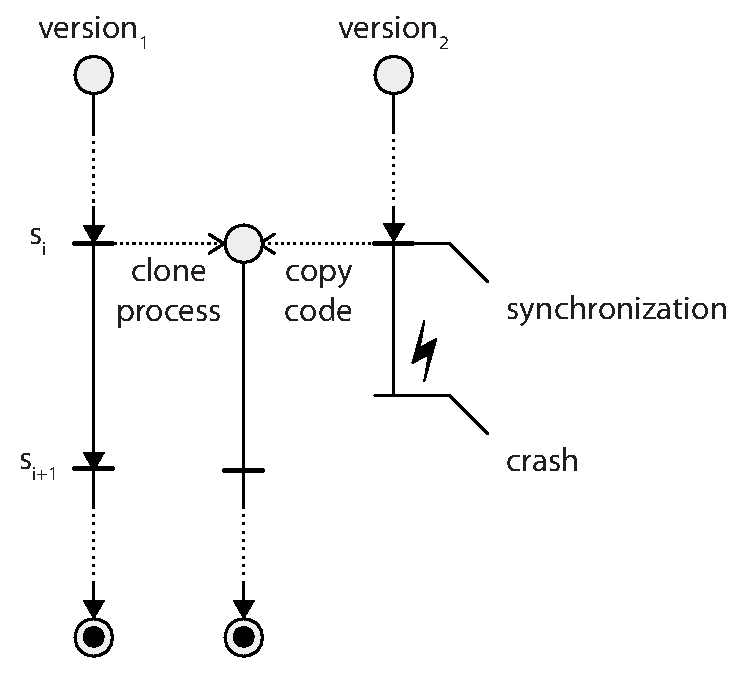
\includegraphics[width=0.45\columnwidth]{safe-updates/figures/solution2}
%%     \label{fig:solution2}
%%   }
%%   \\
%%   \subfloat[Use the code of older version only to run through critical section]{
%%     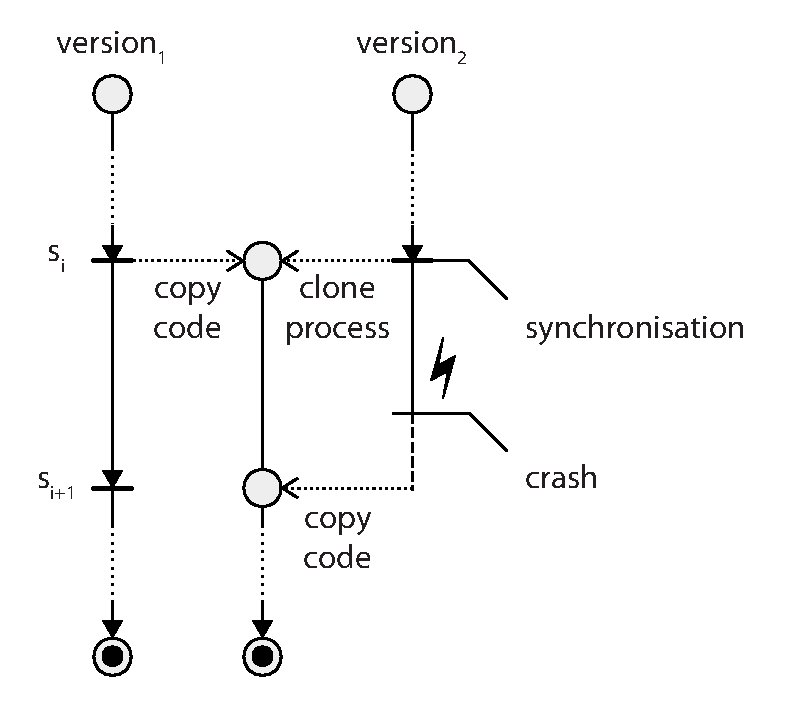
\includegraphics[width=0.45\columnwidth]{safe-updates/figures/solution3}
%%     \label{fig:solution3}
%%   }
%%   \caption{Three solutions for synchronising two divergent versions of
%%   the same application}
%%   \label{fig:solution}
%% \end{figure}

%% \item\label{s1} Clone the correctly executing version to duplicate its state
%%   (\eg memory content, memory mappings) after the crash and replace its
%%   code with the code of the failed version. Then restart both versions and
%%   continue their execution (Figure~\ref{fig:solution1}).

%% \item\label{s2} Clone the correctly executing version to duplicate its state
%%   (\eg memory content, memory mappings) at the last synchronisation point (\ie
%%   creating checkpoint). After the crash, replace the code of this cloned
%%   version with the code of the failed version. Then restart this cloned
%%   version, execute over the \emph{critical section}, and continue execution of
%%   both versions (Figure~\ref{fig:solution2}).

%% \item\label{s3} Clone the failing version to duplicate its state (\eg memory
%%   content, memory mappings) at the last synchronisation point (\ie creating
%%   checkpoint). After the crash, replace the code of this cloned version with
%%   the code of the correctly executing version. Then restart this cloned
%%   version; after the application successfully executes over the \emph{critical
%%   section}, replace the code of the cloned version again with the original
%%   code, and continue its execution (Figure~\ref{fig:solution3}).

%% \end{enumerate}

Our exact recovery mechanism is illustrated in
Figure~\ref{fig:solution3}.  At each system call, \mx creates a
lightweight checkpoint of each version.  This is implemented using the
\lstinline`clone` system call in Linux, which internally uses a
copy-on-write strategy.  
%% As an important optimisation, we omit system
%% calls that can be replayed safely from the last checkpoint, such
%% as \textstt{read}.

As shown in Figure~\ref{fig:solution3}, suppose that the crash happens in
version $v_2$, between system calls $s_1$ and $s_2$.  Then, \rem first restores
$v_2$ at point $s_1$ (\circl{A}), copies $v_1$'s code into $v_2$'s code segment
(\circl{B}), executes over the buggy code using $v_1$'s code (\circl{C}, note
that we are still using $v_2$'s memory state), and then restore $v_2$'s code at
point $s_2$ (\circl{D}).

There are several challenges in implementing this functionality.
First, \rem needs the ability to read and write the application's code
segment.  In the current implementation, we bypass this by linking
together the two application versions after renaming all the symbols
in one of the versions using a modified version of
the \texttt{objcopy}
tool.\footnote{\url{http://sourceware.org/binutils/docs/binutils/objcopy.html}}
However, in the future we plan to implement this transparently by
using the cross-memory attach mechanism used by \mxm.
%% \textstt{pread} and \textstt{pwrite} interface to directly
%% read and write the process memory via the
%% %\textstt{/proc/<pid>/mem} file in the
%% \emph{proc} file system.

%% This functionality has been recently introduced to the Linux kernel in
%% version 2.6.39~\cite{kernel-procmem}; previously, this interface was
%% read-only. This approach imposes only minimal overhead as it allows
%% direct access to the process memory space.

%% The runtime process manipulation functionality is implemented inside
%% \rem, a separate component used by the \mxm monitor. The
%% manipulation itself is driven by the data obtained statically by the
%% \sea analyser before the application has been executed.

Second, \rem needs to modify the contents of the stack in $v_2$.  This is
necessary because the return addresses on the stack frames of $v_2$ still point
to $v_2$'s original code, which was now replaced by $v_1$'s code.  Without also
modifying $v_2$'s stack, any function
\lstinline[language={[x64]Assembler}]`RET` instruction executed between $s_1$
and $s_2$ would most likely veer execution to an incorrect location, since
function addresses are likely to be different across different versions.  Thus,
after \rem replaces $v_2$'s code, it also updates the return addresses on
$v_2$'s stack with the corresponding return addresses in $v_1$, which are
obtained via static analysis (\S\ref{sec:sea}).  Because system calls are
invoked via wrapper functions in C library, this ensures that when $v_2$
resumes execution, it will immediately return to the code in $v_1$.
%% \rem obtains these addresses by analysing $v_1$'s stack at
%% position $s_1$ accessible via checkpoint taken at that point.
%
To implement this functionality, \rem makes use of
the \texttt{libunwind}
library,\footnote{\url{http://www.nongnu.org/libunwind/}} which provides a
portable interface for accessing the program stack, for both x86 and
x86-64 architectures. To actually modify the execution stack of
$v_2$, \rem uses again the \ptrace interface.


Unfortunately, updating the stack return addresses is not sufficient
to ensure that $v_2$ uses $v_1$'s code between $s_1$ and $s_2$, as
$v_2$ may also use function pointers to make function calls.
%% Note that we are still using the $v_2$ memory state. Thereby, $v_2$
%% may still issue a function call to the original code through one of
%% the function pointers.
To handle such cases, \rem inserts breakpoints to the first
instruction of every function in $v_2$'s original code.  Then, when a
breakpoint is encountered, \rem is notified via a \lstinline`SIGTRAP`
signal, and redirects execution to the equivalent function in $v_1$'s
code (which is obtained from the \sea component) by simply changing
the instruction pointer.
%The address of the equivalent function is obtained

Finally, after executing through the buggy code, \rem performs the
same operations in reverse: it redirects execution to $v_2$'s original
code, changes the return addresses on the stack to point to $v_2$'s
functions, and disables all breakpoints inserted in $v_2$'s code.  
The one additional operation that is done at this point is to copy all
the global data modified by $v_1$'s code into the corresponding
locations referenced by $v_2$'s code.  

%\paragraph{Runtime stack analysis and manipulation.}

%% For example, on the x86 architecture, the stack can be easily
%% traversed starting from the top as each stack frame contains frame
%% pointer pointing to the previous stack frame, thereby forming a linked
%% list-like structure. This is not possible on the x86-64 architecture
%% as the frame pointer is no longer stored inside the stack frame.  To
%% traverse the execution stack on this architecture, it is necessary to
%% compute sizes of all functions' stack frames using the stack usage
%% information stored in the \texttt{UNWIND\_CODE} section, which is a
%% part of the ELF binary file. This logic is implemented by the
%% \texttt{libunwind} library, which provides API to unwind the stack
%% independent of the target platform.

%The necessary information about the stack location (\ie address range) and
%page mapping are obtained through the \emph{proc} file system; in particular
%the \textstt{/proc/<pid>/maps} and \textstt{/proc/<pid>/pagemap} files.

Note that \mx cannot currently handle major modifications to the
layout of the data structures used by the code, including individual
stack frames.  While this still allows us to support several common
software update scenarios, in future work we plan to improve the
system with the ability to perform full stack
reconstruction~\cite{upstare} and automatically infer basic data
structure changes at the binary-level~\cite{data-struct-digging}.
%% to identify changes to function names and sequences of function calls
%% (e.g., via clone detection techniques~\cite{cp-miner06,deckard07}),


Our approach of using the code of the non-crashing version to survive failures
in the crashing version may potentially leave the recovered version in an
inconsistent state. However, \mx is able to discover most internal state
inconsistencies by checking whether the two versions have the same external
behaviour after recovery. When the behaviour of the recovered version starts to
differ, \mx will immediately discard it and continue with only one version. The
discarded version can be later restarted at a convenient synchronisation point.
This restarting functionality is not currently implemented in \mx, but we plan
to add it as a future extension.

%Our approach of using the code of the non-crashing version to survive
%failures in the crashing one may leave the application in an
%inconsistent state, and thus may not be applicable for application in
%which absolute correctness and a fail-fast approach are more important
%than allowing the application to survive errors.  However, \mx is
%usually able to discover most internal state inconsistencies, since it
%regularly checks if the two versions have the same external
%behaviour. (See \S\ref{sec:discussion} for an extended discussion.)

\subsection{Binary static analysis}
\label{sec:sea}

%% \begin{table*}[t]
%% \centering 
%% \begin{tabular}{ccc}
%%   \hline
%%   Library calls in $\mathrm{version}_1$ & Library calls in $\mathrm{version}_2$ &
%%   System calls within the library \\
%%   \hline
%%   \texttt{<0xdeadbe5a>} & \texttt{<0xdeadbe8e>} &
%%   [\texttt{<0x77ff2c>}, \texttt{<0x77ffae>}] \\
%%   \texttt{<0xdeadabf5>} & \texttt{<0xdeadac34>} &
%%   [\texttt{<0x782bae>}] \\
%%   \vdots & \vdots & \vdots \\
%% \end{tabular}
%% \caption{Addresses of library function calls, and system calls invoked from
%% within these functions.}
%% \label{tab:syscall_table}
%% \end{table*}

The \sea component statically analyses the binaries of the two
versions to obtain information needed at runtime by the \rem
component.  \sea is invoked only once, when the multi-version
application is assembled from its component versions.
%% As mentioned in \sref{sec:rem}, we currently link together the
%% two application versions after renaming all the symbols in one of them
%% using a modified copy of the \textstt{objcopy} tool, although in the
%% future we plan to do this linking dynamically by directly changing the
%% code segment in each version.

The main goal of \sea is to create several mappings from the code of
one version to the code of the other.  First, \sea extracts the
addresses of all function symbols
in one version and maps them to the
addresses of the corresponding functions in the other version.  This
mapping is used by \rem to handle calls performed via function
pointers (\S\ref{sec:rem}).

Second, \sea computes a mapping from all possible return addresses in
one version to the corresponding return addresses in the other version.  In
order to allow for code changes, this mapping is done by computing an
ordered list of all possible return addresses in each function.  For
example, if function \lstinline`foo` in $v_1$ performs call instructions
at addresses \lstinline`0xabcd0000` and \lstinline`0xabcd0100`, and
function \lstinline`foo` in $v_2$ performs call instructions at
addresses \lstinline`0xdcba0000` and \lstinline`0xdcba0400`, then \sea
will compute the mapping \texttt{\{0xabcd0005 $\rightarrow$
0xdcba0005, 0xabcd0105 $\rightarrow$ 0xdcba0405\}} (assuming each call
instruction takes 5 bytes).  This mapping is then used by \rem to
rewrite return addresses on the stack.

%% These data are gathered by the \sea analyser component which
%% implements static analysis of binary executables to extract all
%% necessary addresses and provide them to other components inside our
%% system. The format used for storing these data is represented by a
%% \emph{call table}. For each version, this table contains addresses of
%% all calls to shared library functions together with the list of all
%% system calls addresses invoked within these library functions, as can
%% be seen in Table~\ref{tab:syscall_table}.

%% For example, the first line of this table represents a call to a
%% library function which does two system calls, while second line
%% represents a function call which does only one system call.

To construct these tables, \sea first needs to extract the addresses
of all function symbols and then disassemble the code for each
individual function in order to locate the call instructions within
them.  The implementation is based on the \texttt{libbfd}
and \texttt{libopcodes} libraries, which are 
part of the
\gnu \binutils suite.\footnote{\url{http://www.gnu.org/software/binutils/}}
To obtain the addresses of all function symbols defined by the
program, \sea uses \texttt{libbfd} to extract the static and dynamic
symbol tables and relocation tables.  To disassemble individual
functions, \sea uses the \texttt{libbf}
library~\cite{kwan:libbf}, built on top of \texttt{libopcodes}.

%% Disassembled machine code is stored in a graph-like structure where
%% individual instructions represents vertices and edges between these
%% vertices represents the control flow. 

%% \paragraph{System call identification.}
%% \sea implementation uses the disassembler to obtain machine
%% code of each individual function and iterates over its instructions
%% (traversing the instruction graph) to identify basic blocks and locate
%% system call instructions within the code these functions.

%% To locate system calls within shared library function calls,
%% \sea first needs to obtain the set of exported library
%% functions and system calls within these functions using the above
%% described approach. Then, \sea analyses the application binary
%% itself and locates all function calls to the shared library using the
%% information extracted from relocation and procedure lookup tables
%% contained in ELF binaries.

%% Results of this analysis are stored in a hash table and tree structure
%% to allow quick access eliminating any unnecessary overhead when these
%% information are accessed during runtime. These data are then used to
%% construct the already described \emph{call table}, before the
%% application itself is executed.

%% \subsection{Limitations and Future Work}
%% \label{sec:limitations}
%% \input{limitations}


\section{Safe software updates}

\section{Parallel software execution}

\section{Scenarios}
\label{nversion-updates:motivation}

In this section we motivate our approach using existing scenarios
involving the \chrome browser and the \vim editor, as well as the \lighttpd
and \vsftpd servers.  These correspond to two categories of
applications that could benefit from our multi-version software update
approach: desktop applications such as web browsers and office tools
for which reliability is a key concern; and network servers, with
stringent security and dependability requirements.

%% We also believe, that the proposed approach might facilitate and
%% improve the
%% \emph{continuous deployment} technique. While this technique has been
%% frequently proposed and advocated in the software engineering community
%% because it encourages experimentation, innovation, and rapid
%% iteration~\cite{johnson2009,harmess2009,linden2009}, its use is still limited
%% since updates may introduce new bugs and security vulnerabilities.  We believe
%% that our approach provides all the benefits of continuous deployment without
%% compromising software reliability.

%\subsection{Google Chrome Web Browser}
%\label{sub:chrome}

\gchrome\footnote{\url{http://www.google.com/chrome}} is one of the most widely 
used web browsers.  Even though \chrome releases are tested
extensively before deployment, they sometimes introduce new bugs that
affect the stability of the browser.  A concrete example is version
$6.0.466.0$, which introduced a bug that caused \chrome to crash when
trying to load certain web pages over
SSL.\footnote{\url{http://code.google.com/p/chromium/issues/detail?id=49197}}
One might argue that in this case the user should downgrade to an
older version and wait until the bug is fixed. However, versions
immediately preceding $6.0.466.0$ suffer from a different
bug,\footnote{\url{http://code.google.com/p/chromium/issues/detail?id=49721}}
which was introduced in version $6.0.438.0$ and which crashes Chrome
during certain sequences of repeated back and forward navigation.

\vim\footnote{\url{http://www.vim.org/}} is arguably one of the most popular 
editors under UNIX.  In version $7.1.127$, while trying to fix a
memory leak, \vim developers introduced a double \textstt{free} bug
that caused \vim to crash whenever the user tried to use a path
completion feature.  This bug made its way into \textit{Ubuntu}
$8.04$, affecting a large number of
users.\footnote{\url{https://bugs.launchpad.net/ubuntu/+source/vim/+bug/219546}}
%% This bug remained undetected until version $7.1.138$, which has been
%% distributed with Ubuntu $8.04$ one of the most popular Linux
%% distributions.  The bug was caused by a

\lighttpd\footnote{\url{http://www.lighttpd.net/}} is a popular 
web-server used by several high-traffic websites such as YouTube,
Wikipedia, and Meebo. Despite its popularity, faulty updates are still
a common occurrence in \lighttpd.
%, as evident from its bug tracking database. 
As one example, a patch introduced in April
2009\footnote{\url{http://redmine.lighttpd.net/projects/lighttpd/repository/revisions/2438}}
(correctly) fixed the way HTTP ETags are computed.
%% The patch was a one-line change, which discarded the terminating zero
%% when computing a hash.
Unfortunately, this fix broke the support for compression, which
relied on the previous way in which ETags were computed and resulted in
a segmentation fault whenever a client requested HTTP compression.
This issue was only 
diagnosed and reported in March
2010\footnote{\url{http://redmine.lighttpd.net/issues/2169}} and
fixed at the end of April 2010,\footnote{\url{http://redmine.lighttpd.net/projects/lighttpd/repository/revisions/2723}} more than one
year after it was introduced, leaving the server vulnerable to
possible attacks in between.

\vsftpd\footnote{\url{https://security.appspot.com/vsftpd.html}} is a fast and 
secure FTP server for UNIX systems.  Version $2.2.0$ added several new
features such as network isolation, but unfortunately also introduced
a
bug\footnote{\url{https://bugs.launchpad.net/ubuntu/+source/vsftpd/+bug/462749}}
which triggered a segmentation fault whenever a client used the
passive FTP mode.  This bug made \vsftpd practically unusable since
the passive mode is being frequently used by clients behind firewalls.
Despite being reported several times, this bug was only fixed in
version $2.2.1$, released more than two months after the bug was
introduced.
%% This is even more surprising given that the bug was triggered by a
%% missing data structure allocation in the newly introduced
%% configuration processing and the patch for this bug consists of a
%% single line.


All the scenarios presented above describe software updates which,
while trying to add new features or bug fixes, also introduced new
bugs that caused the code to crash under certain conditions.
Improving the reliability of such updates is the main goal of our
proposed approach: running both the old and the new version in
parallel after an update can enable applications to survive more
errors, without giving up the new features introduced by the update.

%\section{N-version Updates}
%\input{background/nversion-updates}

%\section{Safe Software Updates}
%\chapter{Multi-version Software Updates}
\label{chap:safe-updates}

% Software updates are an integral part of the software maintenance
% process, with new software versions being released on a continuous
% basis.  Unfortunately, software updates often result in failures,
% which makes many users reluctant to incorporate the latest patches
% made available by developers.  As a result, users rely instead on
% outdated versions, which despite their relative stability, miss recent
% features and bug fixes and may be plagued by security vulnerabilities.

% One of the main reasons for which users hesitate to install updates is
% that a significant number of them result in failures.  It is only too
% easy to find examples of updates that fix a bug or a security
% vulnerability only to introduce another problem in 
% the code. Our goal is to improve the software update
% process in such a way as to encourage users to upgrade to the latest
% software version, without sacrificing the stability of the older
% version.

Multi-version execution can be used to improve the reliability of updated
software by running multiple different versions (revisions) in parallel,
discarding one (or more) versions in case of failure. The potential problem
of such approach is that we might run out of alive versions given multiple
crash bugs located in different parts of the application. We tackle this
problem by combining a multi-version execution with a fail-recovery mechanism
which takes an advantage of the similarity between consecutive software
versions.

% We tackle this problem using a simple but effective multi-version
% based approach.  Whenever a new update becomes available, instead of
% upgrading the software to the new version, we run the new version in
% parallel with the old one; by carefully coordinating their executions
% and selecting the behaviour of the more reliable version when they
% diverge, we create a more secure and dependable multi-version
% application.

We implemented this approach in a prototype system called \mx, which
targets crash bugs in Linux applications
%running on multi-core processors.
\mx allows a new and an old version of an application to
run concurrently, without requiring any
modifications to the application itself or the operating system, nor any
input from the user. To achieve this goal, \mx combines static and
dynamic techniques: it uses static analysis at the binary-level to
construct mappings between the old and the new versions, and synchronizes
execution of the two versions at the system call level, using system call
interposition and synchronisation.  When one of the versions crashes, \mx
transparently restarts it via a lightweight checkpointing mechanism and often
allows it to survive the bug by using the code of the other version.

% We evaluate \mx by showing that it can successfully survive crashes in
% several real applications, specifically several \coreutils utilities and
% two popular servers, \lighttpd and \redis.

%Software systems are constantly evolving, with new versions and
%patches being released on a continuous basis.  Unfortunately, software
%updates present a high risk, with many releases introducing new bugs
%and security vulnerabilities.

%% Applicable in a variety of scenarios, example of one such
%% application might be the desktop and office software where users
%% care about reliability more than performance or efficiency.
%% Examples of such scenarios are provided further in this
%% section. Another application might be the software systems where
%% reliability is critically important, such as web servers,
%% databases, \etc

%% We also believe, that the proposed approach might facilitate and
%% improve the \emph{continuous deployment} technique. While this
%% technique has been frequently proposed and advocated in the
%% software engineering community because it encourages
%% experimentation, innovation, and rapid
%% iteration~\cite{johnson2009,harmess2009,linden2009}, its use is
%% still limited since updates may introduce new bugs and security
%% vulnerabilities.  We believe that our approach provides all the
%% benefits of continuous deployment without compromising software
%% reliability.

To motivate our approach, we present a real scenario involving
\lighttpd, which is representative of one type of applications which
could benefit from our approach, namely server applications with
stringent security and availability requirements.


%% that achieves high-scalability, without sacrificing
%% standards-compliance and security having a small-memory footprint
%% and a small CPU load.  As a result, \lighttpd is
\lighttpd\footnote{\url{http://www.lighttpd.net/}} is a popular open-source 
web-server used 
%(either alone or in conjunction with other web-servers)
by several high-traffic websites such as Wikipedia and Xkcd.
Despite its popularity, crash bugs are still a common
occurrence in \lighttpd, as evident from its bug tracking
database.\footnote{\url{http://redmine.lighttpd.net/issues/}}  Below
we discuss one such bug, which our approach could successfully
eliminate.

%% In October 2008, a bug was reported in \lighttpd affecting the HTTP
%% ETag
%% functionality\footnote{\url{http://redmine.lighttpd.net/issues/1800}}.
%% An ETag a fingerprint assigned by a web server to a specific version
%% of a web resource, which can be used to quickly determine if the
%% resource has changed.  The bug in \lighttpd was that invalid ETags
%% were generated when compression was used.  The bug was fixed in
%% revision
%% 2386\footnote{\url{http://redmine.lighttpd.net/projects/lighttpd/repository/revisions/2386}},

% April 9th 2009
In April 2009, a patch was
applied\footnote{\url{http://redmine.lighttpd.net/projects/lighttpd/repository/revisions/2438}}
to \lighttpd's code related to the HTTP ETag functionality.  An ETag
is a unique string assigned by a web server to a specific version of a
web resource, which can be used to quickly determine if the resource
has changed.  The patch was a one-line change, which discarded the
terminating zero when computing a hash representing the ETag.  More
exactly, line 47 in \textstt{etag.c}:

\begin{lstlisting}[numbers=none,breaklines=true,xleftmargin=0pt]
for (h=0, i=0; i < etag->used; ++i) h = (h<<5)^(h>>27)^(etag->ptr[i]);
\end{lstlisting}
\noindent was changed to:
\begin{lstlisting}[numbers=none,breaklines=true,xleftmargin=0pt]
for (h=0, i=0; i < etag->used@-1@; ++i) h = (h<<5)^(h>>27)^(etag->ptr[i]);
\end{lstlisting}

This correctly changed the way ETags are computed, but unfortunately,
it broke the support for compression, whose implementation depended on
the previous computation.  More precisely, \lighttpd's support for HTTP
compression uses caching to avoid re-compressing files which have not
changed since the last access.  To determine whether the cached
file is still valid, \lighttpd internally uses ETags.  Unfortunately,
the code implementing HTTP compression did not consider the case when
ETags are disabled.  In this case, \textstt{etags->used}
is \textstt{0}, and when the line above is
executed, \textstt{etag->used-1} underflows to a very large value, and
the code crashes while accessing \textstt{etag->ptr[i]}.
Interestingly enough, the original code was still buggy (it always
returns zero as the hash value, and thus it would never re-compress
the files), but it was not vulnerable to a crash. %denial of service
                                                  %attack.

%% \begin{figure}
%% \centering
%% \includegraphics[width=0.9\columnwidth]{safe-updates/figures/lighttpd-scenario}
%% \caption{Crash bug \#2169 from {\footnotesize \texttt{lighttpd}}.}
%% \label{fig:lighttpd-history}
%% \end{figure}

% 8 March
The segfault was diagnosed and reported in March
2010\footnote{\url{http://redmine.lighttpd.net/issues/2169}} and fixed
at the end of April
2010,\footnote{\url{http://redmine.lighttpd.net/projects/lighttpd/repository/revisions/2723}}
more than one year after it was introduced.  
%The history is depicted graphically in Figure~\ref{fig:lighttpd-history}.  
The bottom line is
that for about one year, users affected by this buggy patch
essentially had to decide between%
\begin{inparaenum}[(1)]
\item incorporating the new features
and bug fixes added to the code, but being vulnerable to this crash
bug, and
\item giving up on these new features and bug fixes and using
an old version of \lighttpd, which is not vulnerable to this bug.
\end{inparaenum}
Note that this is particularly true for the eleven-month period
between the time when the bug was introduced and the time it was
diagnosed, since during this period most users would not know how to
change the server's configuration to avoid the crash.

%% The original code, which can be seen in Listing~\ref{lst:2437}, makes the
%% \texttt{i < etag->used} comparison (line 4). Because both \texttt{i} and
%% \texttt{etag->used} are $0$, the condition \texttt{0 < 0} does not hold and
%% the loop body will never be executed.

%% The affected code can be seen in Listing~\ref{lst:2438}. Here, the condition
%% has been changed and comparison has now the form \texttt{i < etag->used-1}.
%% When executing, the \texttt{etag->used} variable will underflow and condition
%% \texttt{0 < 4294967295} will be true. Therefore, the loop body will be
%% executed and access to \texttt{etag->ptr[0]} will result in segmentation
%% fault.

Our approach provides users with a third choice; when a new version
arrives, instead of replacing the old version, we run both versions in
parallel. In our example, consider that we are using \mx to run a
version of \lighttpd from March 2009.  When the buggy April 2010 version
is released, \mx runs it in parallel with the old one.  As the two
versions execute:

\begin{itemize}
\item As long as the two versions have the same external behaviour (\eg they 
write the same values into the same files, or send the same data over
the network), they are run side-by-side and \mx ensures that they act
as one to the outside world (see \S\ref{sec:mxm});

\item{When one of the versions crashes (\eg the new version executes 
the buggy patch), \mx will patch the crashing version at runtime using
the behaviour of the non-crashing version 
(see \S\ref{sec:rem})}.  In this way, \mx can successfully survive
crash bugs in both the old and the new version, increasing the
reliability and availability of the overall application;\looseness=-1

\item When a non-crashing divergence is detected, \mx will discard one of
the versions (by default the old one, but other heuristics can be
used).  The other version can be later restarted at a convenient
synchronisation point (\eg at the beginning of the dispatch loop of
a network server).

\end{itemize}

%% When the two versions diverge because of the newly introduced bug
%% and the April 2010 version crashes, \mx will patch the crashing
%% version at runtime using the behaviour of the non-crashing
%% version. While the recovered version continues to execute, \mx uses
%% the correctly executing March 2009 version as an oracle to ensure
%% that its behaviour is correct. When any divergence is detected, \mx
%% will discard the recovered version and continue using only the old
%% version to ensure correctness. If the divergence is detected
%% during the normal execution, \mx will by default prefer the
%% behaviour of the newer version, but other heuristics can be used as
%% well.

From the user's point of view, this process is completely transparent
and does not cause any interruption in service. In our example, this
effectively eliminates the bug in \lighttpd, while still allowing
users to use the latest features and bug fixes of the recent versions.

%In our proposed approach, when a new version arrives, instead of
%replacing the old version, we run both versions in parallel.  As more
%versions arrive, we execute them in parallel with the existing ones,
%until all available resources have been exhausted, at which point we
%discard some of the versions according to some strategy.

%In our example, consider a system that is running a version
%of \lighttpd from March 2009.  When the buggy April 2010 version is
%released, our system runs it in parallel with the old one.  As the two
%versions execute, the system checks that their external behaviour is
%identical (\eg they write the same values into the same files, or send
%the same data over the network).  When the two versions diverge, the
%divergence is resolved in the favour of the more reliable version.  In
%particular, if one of the two versions crashes, the behaviour of the
%non-crashing version is used, and the other version is transparently
%modified to survive the crash. (Note that the last point is of key
%importance, as the success of our technique depends on having all
%versions running at all times.)  If the system cannot determine which
%behaviour is correct, a simple heuristic can be used, such as always
%preferring the behaviour of the newer version.  In our example, this
%effectively eliminates the bug in \lighttpd, while still allowing
%users to use the latest features and bug fixes of the recent versions.

%Figure~\ref{fig:lighttpd-history}, 


%% Bug 1800: not really using it
%%
%% The bug \#1800 was also related to the HTTP compression and ETag functionality; in
%% particular, invalid ETags were generated for compressed variants of the same
%% resource. The solution for this bug did not consider the situation when
%% ETag support is completely disabled. However, due to an incorrect implementation
%% of ETag hash function, this bug remain undetected until the revision
%% \texttt{2438} when ETag hash function has been fixed.

%% The \texttt{mod\_compress} module implementing the HTTP compression support
%% uses caching to avoid re-compression of files which has been already
%% compressed in the past. To determine whether the cached file is still valid,
%% \texttt{mod\_compress} internally uses ETag stored along with the file.

%% Then, when request for a file is made, \texttt{mod\_compress} module
%% implementation shown in Listing~\ref{lst:2386} first reads the physical file
%% along with its ETag (line 4) and tries to match this ETag with the original
%% one (line 9). However, if ETag support has been disabled, the ETag of the
%% physical file would be empty.

%% \begin{lstlisting}[label=lst:2386,caption={Refactored failing version of the function}]
%% PHYSICALPATH_FUNC(mod_compress_physical) {
%%   stat_cache_entry *sce = NULL;
%%   ...
%%   if (HANDLER_ERROR == stat_cache_get_entry(srv, con, con->physical.path, &sce)) {
%%     ...
%%   }
%%   ...
%%   /* try matching original etag of uncompressed version */
%%   etag_mutate(con->physical.etag, sce->etag);
%%   ...
%% }
%% \end{lstlisting}

%% The original code, which can be seen in Listing~\ref{lst:2437}, makes the
%% \texttt{i < etag->used} comparison (line 4). Because both \texttt{i} and
%% \texttt{etag->used} are $0$, the condition \texttt{0 < 0} does not hold and
%% the loop body will never be executed.

%% The affected code can be seen in Listing~\ref{lst:2438}. Here, the condition
%% has been changed and comparison has now the form \texttt{i < etag->used-1}.
%% When executing, the \texttt{etag->used} variable will underflow and condition
%% \texttt{0 < 4294967295} will be true. Therefore, the loop body will be
%% executed and access to \texttt{etag->ptr[0]} will result in segmentation
%% fault.

%% \begin{lstlisting}[label=lst:2437,caption={Original version of \texttt{etag\_mutate} function}]
%% int etag_mutate(buffer *mut, buffer *etag) {
%%   size_t i;
%%   uint32_t h;
%%   for (h=0, i=0; i < etag->used; ++i) h = (h<<5)^(h>>27)^(etag->ptr[i]);
%%   buffer_reset(mut);
%%   buffer_copy_string_len(mut, CONST_STR_LEN("\""));
%%   buffer_append_long(mut, h);
%%   buffer_append_string_len(mut, CONST_STR_LEN("\""));
%%   return 0;
%% }
%% \end{lstlisting}

%% \begin{lstlisting}[label=lst:2438,caption={Modified version of \texttt{etag\_mutate} function}]
%% int etag_mutate(buffer *mut, buffer *etag) {
%%   size_t i;
%%   uint32_t h;
%%   for (h=0, i=0; i < etag->used-1; ++i) h = (h<<5)^(h>>27)^(etag->ptr[i]);
%%   buffer_reset(mut);
%%   buffer_copy_string_len(mut, CONST_STR_LEN("\""));
%%   buffer_append_long(mut, h);
%%   buffer_append_string_len(mut, CONST_STR_LEN("\""));
%%   return 0;
%% }
%% \end{lstlisting}

\section{Prototype}
\label{sec:mx}

%% \begin{figure}[t!]
%% \centering
%% \includegraphics[width=\columnwidth]{safe-updates/figures/overview}
%% \caption{A platform running both conventional and multi-version
%%   applications.}
%% \label{fig:mx-platform}
%% \end{figure}

We have implemented our approach in a prototype system called \mx,
targeted at multi-core processors running Linux.  Currently, \mx
supports two versions run in parallel. The system works directly on
application binaries, making it easy to deploy it and possibly integrate
it with existing software package managers such as \texttt{apt} or
\texttt{yum}.

%Figure~\ref{fig:mx-platform} shows a platform running \mx, on which
On a platform using \mx, conventional (\ie unmodified) applications
and multi-version (\mv) applications run side by side.  The key
property that must hold on such a platform is that without purposely
trying to do so, applications should not be able to distinguish
between conventional and \mv applications running on the platform. In
particular, the multiple versions of an \mv application should appear
as one to any other entity interacting with them (\eg user, operating
system, other machines).  Furthermore, \mv applications should be more
reliable and secure than their component versions, and their
performance should not be significantly degraded.

To achieve these goals, our prototype \mx employs several different
components, as shown in the architectural overview of
Figure~\ref{fig:design}.  The input to \mx consists of the binaries of
two versions of an application, which we will refer to as 
\textit{the old version}---the one already running on the system, and 
\textit{the new version}---the one newly released.


These two binaries are first statically analysed by the \sea (Static
Executable Analyser) component, which constructs a mapping from the
control flow graph (CFG) of the old version to the CFG of the new
version (\S\ref{sec:sea}).  The two versions are then passed to \mxm
(Multi-eXecution Monitor), whose job is to run the two versions in
parallel, synchronise their execution, virtualise their interaction
with the outside environment, and detect any divergences in their
external behaviour (\S\ref{sec:mxm}).  Once a divergence is detected,
it is resolved by \rem (Runtime Execution Manipulator), which selects
between the available behaviours, and resynchronises the two versions
after the divergence (\S\ref{sec:rem}).

The system prototype has been implemented in C with a small amount of
assembly, and the current version has approximately \mxSLOC source
lines of code. The implementation currently supports Linux kernels
3.2.0 and above, running x86 and x86-64 architectures.

The rest of this section describes the main \mx system components and
their implementation in more detail, and discusses how they work
together to support safe software updates.

\begin{figure}[t!]
\begin{center}
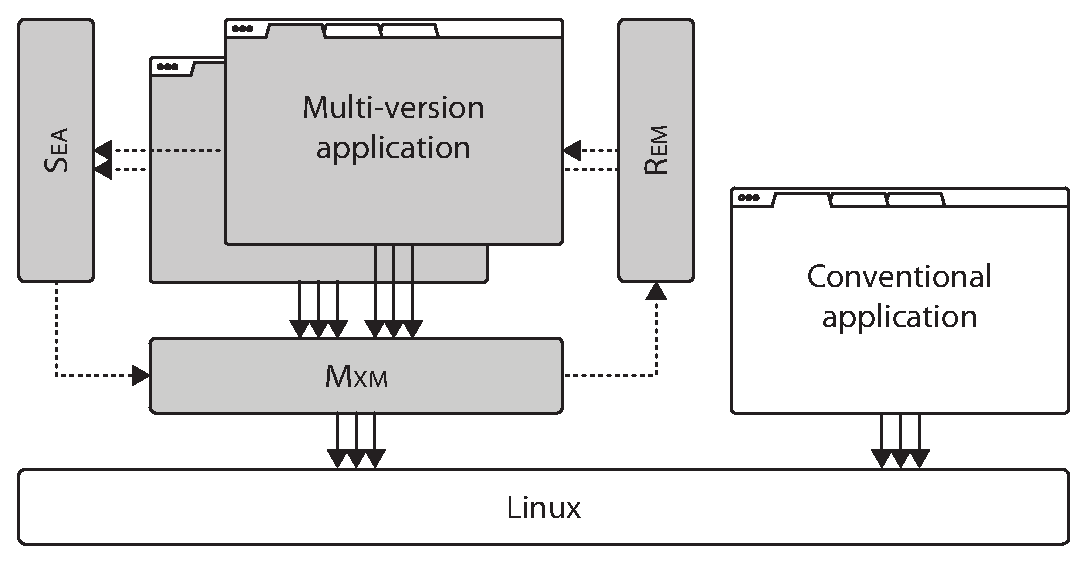
\includegraphics[width=0.6\columnwidth]{safe-updates/figures/architecture}
\caption{\mx system architecture.  
%% The main components of \mx
%%   are \sea (Static Executable Analyser), \mxm (Multi-eXecution
%%   Monitor), and \rem (Runtime Execution Manipulator).
}
\label{fig:design}
\end{center}
\end{figure}


\subsection{System call interposition}
\label{sec:mxm}

One of the main components of our multi-version execution environment
is the \mxm monitor.  \mxm's main jobs are to run the two versions
concurrently, mediate their interaction with the outside world,
synchronise their executions, and detect any divergences in their
external behaviour. \mxm works by intercepting all system calls issued
by each application version, and manipulating them to ensure that the
two versions are executed in a synchronised fashion and act as one to
the outside world.

\mxm provides functionality similar to conventional virtual machine monitors.
Whenever the MV application is executed, the \mxm connects to the two
application versions running in parallel, intercepting their kernel system
calls.  \mxm ensures that the two versions act as one to the outside world by
mediating access to the underlying operating system to achieve complete
isolation of the running application from other application instances as well
as from the external environment, making sure the combined application versions
act as one to the outside world.  The environment controlled by the monitor
consists mainly of a restricted file system access, socket interceptors and
signal handlers.

\subsubsection{System call interception}

\mxm is implemented using the  \ptrace interface provided by the Linux
kernel.  This interface, often used for application debugging, allows
simple deployment (without any need for compile-time instrumentation)
and makes the monitor itself lightweight since it is running as a
regular unprivileged process.  \mxm is similar in operation to previous
monitors whose goal is to synchronise applications at the level of system
calls such as \orchestra~\cite{orchestra09}, PLR~\cite{shye2009} or
\tachyon~\cite{tachyon12}.

\mxm runs each version in a separate child process, intercepting all
their system calls.  When a system call is intercepted in one version,
\mxm waits until the other version also performs a system call.  With
a pair of system calls in hand (one executed by the old version, and
one by the new version), \mxm compares their types and arguments.  If
they differ, \mxm has detected a divergence and invokes the \rem
component to resolve it (\S\ref{sec:rem}).

Otherwise, if the two versions perform the same system call with the
same arguments, \mxm virtualises their interaction with the
environment.  If the operation performed by the system call has no
side effects and does not involve virtualised state (\eg
\lstinline`sysinfo`), \mxm allows both processes to execute it
independently.  Otherwise, it executes the system call on their
behalf and copies its results into the address spaces of both
versions.

\mxm must also enforce deterministic execution across versions. This
consists mainly of intercepting instructions that may produce
non-deterministic results, and returning the same result in both
versions.  Examples of such non-deterministic operations include
random number generators (\eg read calls to \lstinline`/dev/[u]random`),
date and time (\eg read calls to \lstinline`/etc/localtime`), and access
to files and network (\eg file descriptor consistency).  Note that
non-deterministic effects resulting from allocating memory objects at
different addresses in memory or randomly arranging memory areas via
address space layout randomisation (ASLR) do not pose any
problems: \mxm understands the semantics of individual system calls and
rather than directly comparing memory addresses (which might be
different in each executed version), it compares the actual values
stored at those memory locations. \mxm supports both memory buffers (by
comparing the actual buffer content) as well as data structures
referenced by pointers (including nested ones).
 
Since \mxm fully controls executing programs intercepting all their system
calls, it can ensure that both programs have the same view of their
environment. Whenever the monitored process makes a system call, \mxm is
notified twice---first before, then after the call has been executed.  When a
\ptrace event is raised (\eg a new child process has been started), the monitor
is notified as well.  Due to internal limitations of the \ptrace interface,
once the system call has been made, it cannot be skipped, so when \mxm wants to
execute the call on behalf of its child processes, it simply replaces it with a
system call that does not change the system state (\lstinline`getpid` in our
case).

There are several challenges that we encountered while implementing
\mxm.  First, \mxm must partly understand the semantics of 
system calls.  For example, many system call parameters use complex
(often nested) structures with complicated semantics to pass values to
the operating system kernel, as in the case of \lstinline`ioctl` or
\lstinline`futex`.  To be able to compare the parameters of
these system calls and copy back their results, \mxm needs to
understand the semantics of these structures.  However, there are only
a relatively small number of system calls in Linux, and once the support
for handling them is implemented, it can be reused across applications.
\mxm currently implements \syscallsImplemented system calls (out of the
\syscallsTotal provided by Linux x86-64 3.1.9), which was enough to
allow us to run \mx on our benchmarks
(\S\ref{sec:reliability-evaluation}).

Second, the arguments of a system call are often passed through pointers,
which are only valid in the application address space, which is not directly
available to \mxm.  Therefore, \mxm needs to copy the contents pointed to by
these structures to its own address space in order to perform their
comparison.  The \ptrace interface on x86-64 only allows to copy one quadword
per system call, which is very expensive. Previous approaches either used
various ad-hoc optimisations~\cite{orchestra09} such as named pipes or shared
memory with custom shellcode, or a modified kernel~\cite{tachyon12} to
overcome this limitation. Instead, \mxm uses \emph{cross memory attach}, a new
mechanism for fast interprocess communication which has been recently added to
the Linux kernel~\cite{crossmemoryattach}.  This mechanism provides two new
system calls---\lstinline`process_vm_readv` and
\lstinline`process_vm_writev`---which allows the tracer to directly access the
memory space of the tracee using an interface similar to the \lstinline`readv`
and \lstinline`writev` system calls without any additional overhead.

Third, because the structures passed as arguments to system calls often have
variable size, \mxm also needs a fast way to allocate and deallocate memory
for them in order to minimise the overall overhead imposed by our system.  For
this purpose, \mxm uses a region-based memory allocator~\cite{memory-pools},
namely the \textsf{obstack}
library,\footnote{\url{http://www.gnu.org/software/hello/manual/libc/Obstacks.html}}
which is part of the \gnu C Library.  Each monitored process has its own
region, which is used for allocating memory to store the copy of the process'
system call arguments

\subsubsection{Multi-process and multi-threaded applications}

Finally, a particular challenge arises in the context of multi-process and
multi-threaded applications.  Using a single monitor instance to intercept both
versions and their child processes (or threads) would eliminate any advantage
that these applications derive from using concurrency.  Therefore, \mxm uses a
new monitor thread for each set of child processes (or threads) spawned by the
application.  For instance, if the old and new versions each have a parent and
a child process, then \mxm will use two threads: one to monitor the parent
processes, and one to monitor the child processes in each version.

Due to limitations of the \ptrace interface (which was not designed to be used
in a multi-process or multi-threaded environment), handing the control of any
child processes being spawned by the application over to a new monitoring
thread is somewhat complicated.  In \mxm we adopt a solution similar to
Orchestra~\cite{orchestra09}.  When a new child process is spawned, we let the
parent monitoring thread to supervise its execution until the first system
call.  Then, we replace this system call with a \lstinline`pause` system call,
disconnect the parent monitor (which causes a \lstinline`SIGCONT` signal to be
sent to all new child processes), and spawn a new monitoring thread which
immediately reconnects to the new child process, restores its original system
call, and resumes its execution.

\mxm does not enforce deterministic execution across multiple versions of
multi-threaded programs (which may diverge if race conditions can lead
to different external behaviour across executions), although we could
overcome this limitation by adopting \varan's solution
(\S\ref{sec:threading}).

%% \mxm also performs a series of optimisations to decrease performance
%% overhead, such as allowing certain files with read-only permissions
%% to be opened directly by the process. 

\subsubsection{Environment virtualisation}

To improve I/O performance and decrease virtualisation overhead,
processes are allowed to open files with read-only permissions
directly, while files with write permissions are opened by the monitor
itself.  This imposes another problem as file descriptors assigned to
these files are not necessarily the same in each version (\eg due to
scheduling non-determinism). Therefore, \mxm needs to virtualise
these file descriptors.

Whenever the monitored process opens a file with read-only permissions, a
new virtual file descriptor is assigned to this file together with the
mapping to a real file descriptor for each version. This virtual file
descriptor is then sent to each version. When a system call is made
using this virtual file descriptor, \mxm replaces it with the real
file descriptor before executing the system call. The actual file
operation is then executed by the process itself avoiding any memory
copying by \mxm.

A similar approach is also used for virtualisation of process,
group, parent and child identifiers.  Whenever a process tries to obtain
the actual ID, \mxm replaces this with a virtual ID and keeps the
mapping between the real and the virtual ID. When a process invokes a
system call using this ID as an argument (\eg \lstinline`kill`), the
virtual ID is replaced with the actual ID before executing the system
call.

%% \paragraph{Para-virtualisation interface and binary translation.}
%% Furthermore, we plan to combine this API with a binary translation
%% approach~\cite{binary-translation}, that will allow to dynamically
%% replace certain system calls with more efficient \emph{monitor
%% call} instructions.  The binary translation could be also used to
%% dynamically replace code components that have been proved to be
%% safe and do not need to be replicated across multiple versions (\eg
%% using static verification during compilation, using traces of
%% previous execution, using runtime heuristics).


%% \paragraph{Future work}

%% The \texttt{ptrace} interface allows us to easily monitor the program
%% execution without any compile-time instrumentation.  The main downside
%% of this approach is a relatively high overhead.  This is especially
%% true for I/O intensive applications, as they require frequent
%% transfers of large portions of the application memory space to the
%% monitor process. This overhead could be eliminated by directly
%% accessing the process memory space.

%% The existing prototype implementation of \textsc{Mxm} already supports
%% simple scenarios. The main limitation of this implementation is the
%% strict ordering of system calls, which must be the same in each
%% monitored application version.  To be practically usable, future
%% versions of \textsc{Mxm} need to relax the requirement on strict
%% ordering to allow more complex scenarios. This is especially important
%% when executing different versions of the same application.

%% Most importantly, a straightforward comparison of system call traces
%% is usually not sufficient to identify divergences, since different
%% versions might use a slightly different sequence of kernel and library
%% calls to implement the same behaviour.  We plan to explore approaches
%% similar to those implemented by compiler optimisations, such as
%% \emph{peep-hole optimisation}~\cite{dragon-book}, and adapt them to
%% work on the level of kernel and library calls.


%% %% \paragraph{Hashing system call traces.}
%% %% To decrease the overhead of kernel and library call synchronisation, we aim to
%% %% enhance our system to hash the sequence of system call traces using fast hash
%% %% functions such as FNV-1 or FNV-1a.  This approach has a significant advantage
%% %% over straightforward comparison of call traces, especially in the case of
%% %% system calls with virtually unlimited parameter sizes such as \texttt{read} or
%% %% \texttt{write}~\cite{shye2009}.  Similar approach has been already used
%% %% in~\cite{shye2009}.

%% \paragraph{Libraries support and virtualisation.}
%% Since many applications today use functionality provided by shared
%% libraries, we aim to support intercepting calls to such libraries as
%% well. Moreover, as intercepted calls to shared libraries can be
%% executed only once, same as in the case of system call monitoring,
%% this may decrease the overall overhead of multi-version execution.

%% We also plan to provide our own implementation of the \texttt{libc}
%% library loaded using the \texttt{LD\_PRELOAD} mechanism.  This library
%% will communicate directly with the monitor process through shared
%% memory, decreasing the number of system calls that need to be directly
%% intercepted, and thus resulting in much better performance.  However,
%% since the \texttt{LD\_PRELOAD} mechanism can be overridden, we still
%% need to combine it with the \texttt{ptrace} monitoring facility to
%% achieve complete isolation with reasonable overhead.  This approach
%% can be extended to support other shared libraries as well, further
%% improving the overall performance of our approach.

\subsection{Runtime state manipulation}
\label{sec:rem}

At the core of our system lies the \rem component, which is invoked
by \mxm whenever a divergence is detected.  \rem has two main jobs:
(1)~to decide whether to resolve the divergence in favour of the old or
the new version; and (2)~to allow the other version to execute through
the divergence and resynchronise the execution of the two versions
after the divergence.
%% The first task by itself it's easy: we favour the new version, except
%% for when it crashes.
%% As discussed in \sref{sec:scope}, in this paper we restrict our
%% attention to surviving crash errors, so the first task is relatively
%% easy: if one of the two versions crashes, we use the output of the
%% other version; otherwise, we always favour the new version.  
%%
%% The second task is however more difficult, but essential to the
%% success of our approach, which relies on having both versions be alive
%% at all times, so that the overall application can survive any crash
%% bugs that happen in either the old or the new version (although of
%% course, not in both).
%%
As discussed in Section~\ref{multi-version:rationale}, in \mx we focus
our attention on surviving crash errors, so the key challenge is to
allow the crashing version to survive the crash.  This is essential to
the success of our approach, which relies on having both versions alive
at all times, so that the overall application can survive any crash bugs
that happen in either the old or the new version (although of course,
not in both at the same time).

We emphasise that we apply our approach only to crash errors (those
raising a \lstinline`SIGSEGV` signal), and not to other types of program
termination, such as \lstinline`abort`.  This is important from a
security perspective, because
%% many patches turn potential compromises into
%% run-time {\small{\texttt{abort}s}}, \eg using assertions for input
%% sanitisation.  For example, 
when a vulnerability is discovered, but a proper solution is not yet
known, developers often\footnote{For example, see the patch in \texttt{json-cpp}~\url{http://jsoncpp.svn.sourceforge.net/viewvc/jsoncpp/trunk/jsoncpp/include/json/assertions.h?r1=247&r2=246&pathrev=247}}
fail-stop the program rather than letting it continue and allowing
the attacker to compromise the system.
%
%% Such situations can be easily distinguished since failed assertions
%% result in program abortion (\ie
%% \textstt{SIGABRT} signal), while unintentional program crashes typically
%% result in abnormal termination (\ie \textstt{SIGSEGV} signal). 
%% Therefore, \rem only intercepts and handles crashes resulting
%%   in \textstt{SIGSEGV} signals.

Suppose that one of the versions has crashed between the execution of
system call $s_1$ and the execution of system call $s_2$.  Then, in
many common scenarios, the code executed between the two system calls
is responsible for the crash (\eg the old version crashes because it
doesn't incorporate a bug fix present in the new version, or the new
version crashes because its code was patched incorrectly).  Therefore,
our strategy is to do a form of \textit{runtime code patching}, in
which we use the code of the non-crashing version to execute over the
buggy code in the crashing version.

%% If the behaviour of the two versions is different, but they both
%% continue to execute, then we favour the behaviour of the new version and
%% wait for the two versions to reconverge.

%% There are many different ways to achieve this goal, such as the use of
%% a mechanism based on check-pointing and roll-back~\cite{qin2005};
%% however, these mechanisms cannot deal with persistent errors which are
%% common in the case of software updates.

%% Our solution is based upon the observation that errors in programs are
%% usually located at particular places (\ie specific instructions) in
%% the program's code.  Therefore, we can use the code of the other, and
%% \ie correct, version to execute over this critical point in program's
%% code. This approach may not work when memory layout of the two
%% versions differs, as the code of one version may fail to locate the
%% memory structures necessary for its execution in the memory of the
%% other version. Nevertheless, the described approach might still work
%% in many cases when memory layout of the two versions does not differ
%% significantly.


%\paragraph{Possible execution scenarios.}

%% We run two versions of the same application in parallel, monitoring
%% their execution to be sure that they behave in the same way without
%% any divergences by comparing the application executions at
%% synchronisation points; in case of our prototype equal to system
%% calls. When either of the versions fail, we stop its execution at the
%% \emph{divergence point}; at this point there are three possible
%% solutions to synchronise the divergent versions:

\begin{figure}[t]
\centering
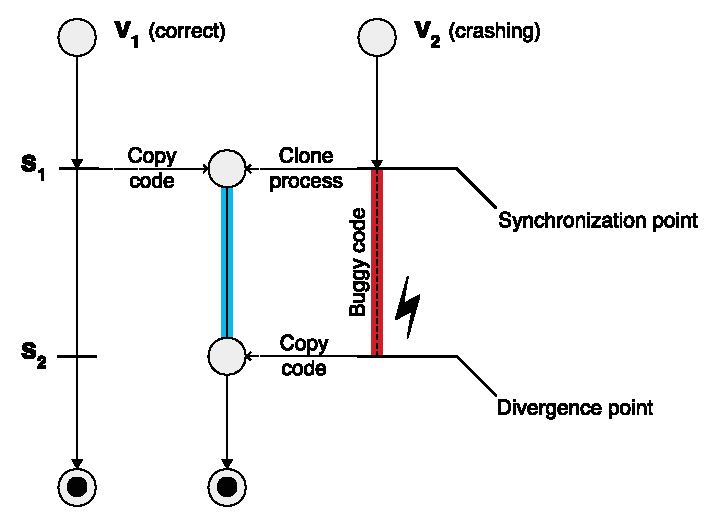
\includegraphics[width=0.5\columnwidth]{safe-updates/figures/strategy}
\caption{\rem's recovery mechanism uses the code of the non-crashing
  version to run through the buggy code.}
\label{fig:solution3}
\end{figure}

%% \begin{enumerate}[label=\emph{S\arabic*}, itemsep=3pt, parsep=3pt]
%% \renewcommand*\labelitemi{\emph{S\arabic*}}
%% \begin{figure}[t]
%%   \centering
%%   \subfloat[Patch state after the crash and continue execution]{
%%     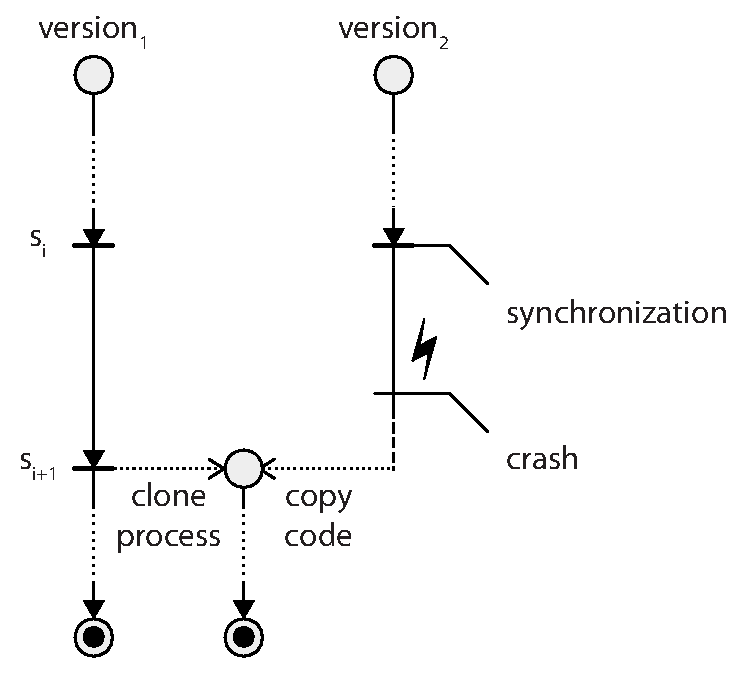
\includegraphics[width=0.45\columnwidth]{safe-updates/figures/solution1}
%%     \label{fig:solution1}
%%   }
%%   \quad
%%   \subfloat[Patch state before the crash and continue execution]{
%%     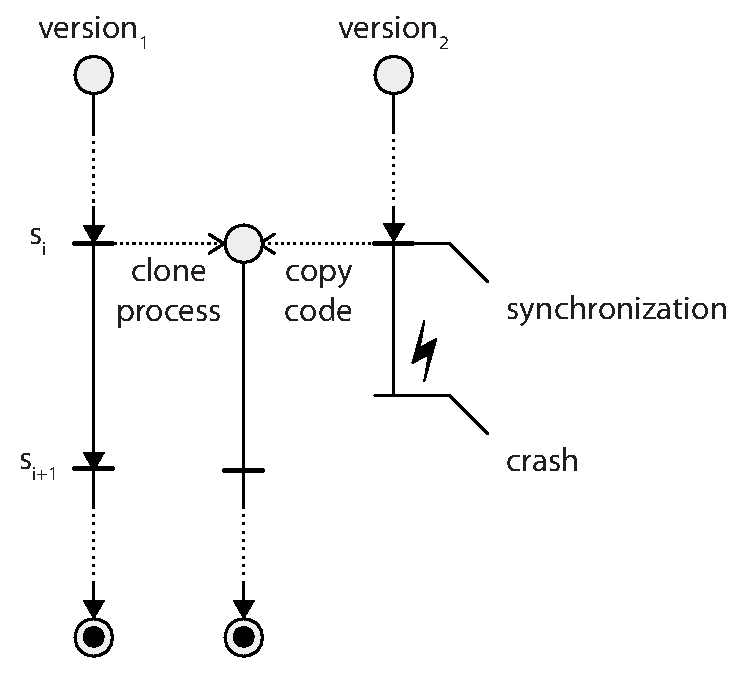
\includegraphics[width=0.45\columnwidth]{safe-updates/figures/solution2}
%%     \label{fig:solution2}
%%   }
%%   \\
%%   \subfloat[Use the code of older version only to run through critical section]{
%%     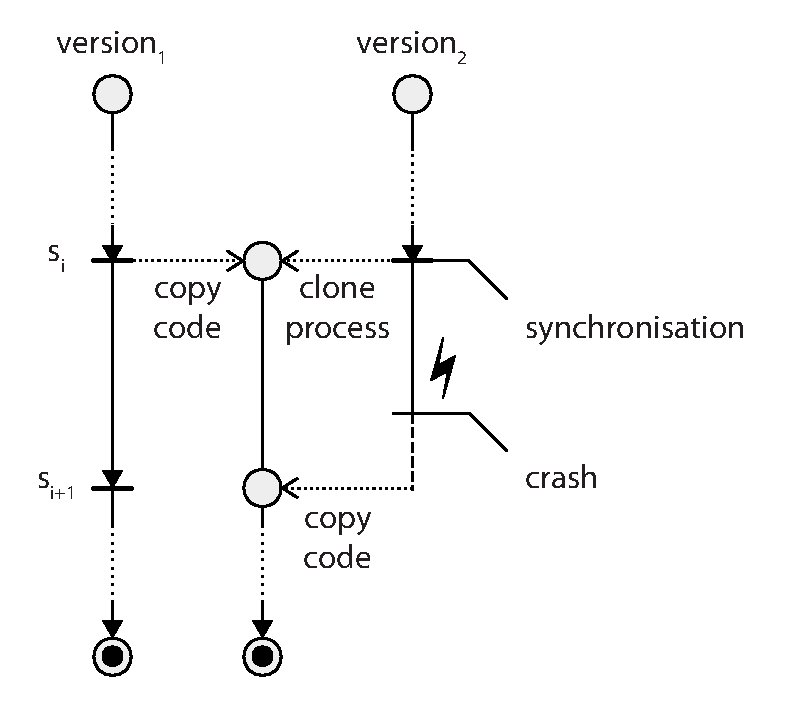
\includegraphics[width=0.45\columnwidth]{safe-updates/figures/solution3}
%%     \label{fig:solution3}
%%   }
%%   \caption{Three solutions for synchronising two divergent versions of
%%   the same application}
%%   \label{fig:solution}
%% \end{figure}

%% \item\label{s1} Clone the correctly executing version to duplicate its state
%%   (\eg memory content, memory mappings) after the crash and replace its
%%   code with the code of the failed version. Then restart both versions and
%%   continue their execution (Figure~\ref{fig:solution1}).

%% \item\label{s2} Clone the correctly executing version to duplicate its state
%%   (\eg memory content, memory mappings) at the last synchronisation point (\ie
%%   creating checkpoint). After the crash, replace the code of this cloned
%%   version with the code of the failed version. Then restart this cloned
%%   version, execute over the \emph{critical section}, and continue execution of
%%   both versions (Figure~\ref{fig:solution2}).

%% \item\label{s3} Clone the failing version to duplicate its state (\eg memory
%%   content, memory mappings) at the last synchronisation point (\ie creating
%%   checkpoint). After the crash, replace the code of this cloned version with
%%   the code of the correctly executing version. Then restart this cloned
%%   version; after the application successfully executes over the \emph{critical
%%   section}, replace the code of the cloned version again with the original
%%   code, and continue its execution (Figure~\ref{fig:solution3}).

%% \end{enumerate}

Our exact recovery mechanism is illustrated in
Figure~\ref{fig:solution3}.  At each system call, \mx creates a
lightweight checkpoint of each version.  This is implemented using the
\lstinline`clone` system call in Linux, which internally uses a
copy-on-write strategy.  
%% As an important optimisation, we omit system
%% calls that can be replayed safely from the last checkpoint, such
%% as \textstt{read}.

As shown in Figure~\ref{fig:solution3}, suppose that the crash happens in
version $v_2$, between system calls $s_1$ and $s_2$.  Then, \rem first restores
$v_2$ at point $s_1$ (\circl{A}), copies $v_1$'s code into $v_2$'s code segment
(\circl{B}), executes over the buggy code using $v_1$'s code (\circl{C}, note
that we are still using $v_2$'s memory state), and then restore $v_2$'s code at
point $s_2$ (\circl{D}).

There are several challenges in implementing this functionality.
First, \rem needs the ability to read and write the application's code
segment.  In the current implementation, we bypass this by linking
together the two application versions after renaming all the symbols
in one of the versions using a modified version of
the \texttt{objcopy}
tool.\footnote{\url{http://sourceware.org/binutils/docs/binutils/objcopy.html}}
However, in the future we plan to implement this transparently by
using the cross-memory attach mechanism used by \mxm.
%% \textstt{pread} and \textstt{pwrite} interface to directly
%% read and write the process memory via the
%% %\textstt{/proc/<pid>/mem} file in the
%% \emph{proc} file system.

%% This functionality has been recently introduced to the Linux kernel in
%% version 2.6.39~\cite{kernel-procmem}; previously, this interface was
%% read-only. This approach imposes only minimal overhead as it allows
%% direct access to the process memory space.

%% The runtime process manipulation functionality is implemented inside
%% \rem, a separate component used by the \mxm monitor. The
%% manipulation itself is driven by the data obtained statically by the
%% \sea analyser before the application has been executed.

Second, \rem needs to modify the contents of the stack in $v_2$.  This is
necessary because the return addresses on the stack frames of $v_2$ still point
to $v_2$'s original code, which was now replaced by $v_1$'s code.  Without also
modifying $v_2$'s stack, any function
\lstinline[language={[x64]Assembler}]`RET` instruction executed between $s_1$
and $s_2$ would most likely veer execution to an incorrect location, since
function addresses are likely to be different across different versions.  Thus,
after \rem replaces $v_2$'s code, it also updates the return addresses on
$v_2$'s stack with the corresponding return addresses in $v_1$, which are
obtained via static analysis (\S\ref{sec:sea}).  Because system calls are
invoked via wrapper functions in C library, this ensures that when $v_2$
resumes execution, it will immediately return to the code in $v_1$.
%% \rem obtains these addresses by analysing $v_1$'s stack at
%% position $s_1$ accessible via checkpoint taken at that point.
%
To implement this functionality, \rem makes use of
the \texttt{libunwind}
library,\footnote{\url{http://www.nongnu.org/libunwind/}} which provides a
portable interface for accessing the program stack, for both x86 and
x86-64 architectures. To actually modify the execution stack of
$v_2$, \rem uses again the \ptrace interface.


Unfortunately, updating the stack return addresses is not sufficient
to ensure that $v_2$ uses $v_1$'s code between $s_1$ and $s_2$, as
$v_2$ may also use function pointers to make function calls.
%% Note that we are still using the $v_2$ memory state. Thereby, $v_2$
%% may still issue a function call to the original code through one of
%% the function pointers.
To handle such cases, \rem inserts breakpoints to the first
instruction of every function in $v_2$'s original code.  Then, when a
breakpoint is encountered, \rem is notified via a \lstinline`SIGTRAP`
signal, and redirects execution to the equivalent function in $v_1$'s
code (which is obtained from the \sea component) by simply changing
the instruction pointer.
%The address of the equivalent function is obtained

Finally, after executing through the buggy code, \rem performs the
same operations in reverse: it redirects execution to $v_2$'s original
code, changes the return addresses on the stack to point to $v_2$'s
functions, and disables all breakpoints inserted in $v_2$'s code.  
The one additional operation that is done at this point is to copy all
the global data modified by $v_1$'s code into the corresponding
locations referenced by $v_2$'s code.  

%\paragraph{Runtime stack analysis and manipulation.}

%% For example, on the x86 architecture, the stack can be easily
%% traversed starting from the top as each stack frame contains frame
%% pointer pointing to the previous stack frame, thereby forming a linked
%% list-like structure. This is not possible on the x86-64 architecture
%% as the frame pointer is no longer stored inside the stack frame.  To
%% traverse the execution stack on this architecture, it is necessary to
%% compute sizes of all functions' stack frames using the stack usage
%% information stored in the \texttt{UNWIND\_CODE} section, which is a
%% part of the ELF binary file. This logic is implemented by the
%% \texttt{libunwind} library, which provides API to unwind the stack
%% independent of the target platform.

%The necessary information about the stack location (\ie address range) and
%page mapping are obtained through the \emph{proc} file system; in particular
%the \textstt{/proc/<pid>/maps} and \textstt{/proc/<pid>/pagemap} files.

Note that \mx cannot currently handle major modifications to the
layout of the data structures used by the code, including individual
stack frames.  While this still allows us to support several common
software update scenarios, in future work we plan to improve the
system with the ability to perform full stack
reconstruction~\cite{upstare} and automatically infer basic data
structure changes at the binary-level~\cite{data-struct-digging}.
%% to identify changes to function names and sequences of function calls
%% (e.g., via clone detection techniques~\cite{cp-miner06,deckard07}),


Our approach of using the code of the non-crashing version to survive failures
in the crashing version may potentially leave the recovered version in an
inconsistent state. However, \mx is able to discover most internal state
inconsistencies by checking whether the two versions have the same external
behaviour after recovery. When the behaviour of the recovered version starts to
differ, \mx will immediately discard it and continue with only one version. The
discarded version can be later restarted at a convenient synchronisation point.
This restarting functionality is not currently implemented in \mx, but we plan
to add it as a future extension.

%Our approach of using the code of the non-crashing version to survive
%failures in the crashing one may leave the application in an
%inconsistent state, and thus may not be applicable for application in
%which absolute correctness and a fail-fast approach are more important
%than allowing the application to survive errors.  However, \mx is
%usually able to discover most internal state inconsistencies, since it
%regularly checks if the two versions have the same external
%behaviour. (See \S\ref{sec:discussion} for an extended discussion.)

\subsection{Binary static analysis}
\label{sec:sea}

%% \begin{table*}[t]
%% \centering 
%% \begin{tabular}{ccc}
%%   \hline
%%   Library calls in $\mathrm{version}_1$ & Library calls in $\mathrm{version}_2$ &
%%   System calls within the library \\
%%   \hline
%%   \texttt{<0xdeadbe5a>} & \texttt{<0xdeadbe8e>} &
%%   [\texttt{<0x77ff2c>}, \texttt{<0x77ffae>}] \\
%%   \texttt{<0xdeadabf5>} & \texttt{<0xdeadac34>} &
%%   [\texttt{<0x782bae>}] \\
%%   \vdots & \vdots & \vdots \\
%% \end{tabular}
%% \caption{Addresses of library function calls, and system calls invoked from
%% within these functions.}
%% \label{tab:syscall_table}
%% \end{table*}

The \sea component statically analyses the binaries of the two
versions to obtain information needed at runtime by the \rem
component.  \sea is invoked only once, when the multi-version
application is assembled from its component versions.
%% As mentioned in \sref{sec:rem}, we currently link together the
%% two application versions after renaming all the symbols in one of them
%% using a modified copy of the \textstt{objcopy} tool, although in the
%% future we plan to do this linking dynamically by directly changing the
%% code segment in each version.

The main goal of \sea is to create several mappings from the code of
one version to the code of the other.  First, \sea extracts the
addresses of all function symbols
in one version and maps them to the
addresses of the corresponding functions in the other version.  This
mapping is used by \rem to handle calls performed via function
pointers (\S\ref{sec:rem}).

Second, \sea computes a mapping from all possible return addresses in
one version to the corresponding return addresses in the other version.  In
order to allow for code changes, this mapping is done by computing an
ordered list of all possible return addresses in each function.  For
example, if function \lstinline`foo` in $v_1$ performs call instructions
at addresses \lstinline`0xabcd0000` and \lstinline`0xabcd0100`, and
function \lstinline`foo` in $v_2$ performs call instructions at
addresses \lstinline`0xdcba0000` and \lstinline`0xdcba0400`, then \sea
will compute the mapping \texttt{\{0xabcd0005 $\rightarrow$
0xdcba0005, 0xabcd0105 $\rightarrow$ 0xdcba0405\}} (assuming each call
instruction takes 5 bytes).  This mapping is then used by \rem to
rewrite return addresses on the stack.

%% These data are gathered by the \sea analyser component which
%% implements static analysis of binary executables to extract all
%% necessary addresses and provide them to other components inside our
%% system. The format used for storing these data is represented by a
%% \emph{call table}. For each version, this table contains addresses of
%% all calls to shared library functions together with the list of all
%% system calls addresses invoked within these library functions, as can
%% be seen in Table~\ref{tab:syscall_table}.

%% For example, the first line of this table represents a call to a
%% library function which does two system calls, while second line
%% represents a function call which does only one system call.

To construct these tables, \sea first needs to extract the addresses
of all function symbols and then disassemble the code for each
individual function in order to locate the call instructions within
them.  The implementation is based on the \texttt{libbfd}
and \texttt{libopcodes} libraries, which are 
part of the
\gnu \binutils suite.\footnote{\url{http://www.gnu.org/software/binutils/}}
To obtain the addresses of all function symbols defined by the
program, \sea uses \texttt{libbfd} to extract the static and dynamic
symbol tables and relocation tables.  To disassemble individual
functions, \sea uses the \texttt{libbf}
library~\cite{kwan:libbf}, built on top of \texttt{libopcodes}.

%% Disassembled machine code is stored in a graph-like structure where
%% individual instructions represents vertices and edges between these
%% vertices represents the control flow. 

%% \paragraph{System call identification.}
%% \sea implementation uses the disassembler to obtain machine
%% code of each individual function and iterates over its instructions
%% (traversing the instruction graph) to identify basic blocks and locate
%% system call instructions within the code these functions.

%% To locate system calls within shared library function calls,
%% \sea first needs to obtain the set of exported library
%% functions and system calls within these functions using the above
%% described approach. Then, \sea analyses the application binary
%% itself and locates all function calls to the shared library using the
%% information extracted from relocation and procedure lookup tables
%% contained in ELF binaries.

%% Results of this analysis are stored in a hash table and tree structure
%% to allow quick access eliminating any unnecessary overhead when these
%% information are accessed during runtime. These data are then used to
%% construct the already described \emph{call table}, before the
%% application itself is executed.

%% \subsection{Limitations and Future Work}
%% \label{sec:limitations}
%% \input{limitations}

\section{Reliability Evaluation}
\label{sec:reliability-evaluation}

To evaluate our approach, we show that \mx can survive crash bugs in several
real applications (\S\ref{sec:surviving}). We then examine the question of how
far apart can be the versions run by \mx (\S\ref{sec:bounds}), and discuss
\mx's performance overhead (\S\ref{sec:performance}).

\subsection{Fault recovery}
\label{sec:surviving}

We have evaluated \mx using a set of bugs in three applications: \gnu
\coreutils, \redis and \lighttpd. We discuss each application in turn below.

\subsubsection{\gnu \coreutils}
\label{sec:coreutils}

\begin{table}[t]
\begin{center}
\caption{Utilities from \gnu \coreutils, the crash bugs used, and the 
versions in which these bugs were introduced and fixed.  We group
together utilities affected by the same or similar bugs.}
\begin{tabular}{lll}
\toprule
\textsc{Utility} & \textsc{Bug description} & \textsc{Bug span} \\
\midrule
\mdsum & \multirow{2}{*}{Buffer underflow} & \multirow{2}{*}{v5.1 -- v6.11} \\
\shasum & & \\
\midrule
\mkdir & \multirow{2}{*}{\textstt{NULL}-pointer dereference} & \multirow{2}{*}{v5.1 -- v6.11} \\
\mkfifo & & \\
\mknod & & \\
\midrule
\cut & Buffer overflow & v5.3 -- v8.11 \\
\bottomrule
\end{tabular}
\label{tbl:cu-bugs}
\end{center}
\end{table}

As an initial evaluation of \mx's ability to survive crashes, we have used
applications from the \gnu \coreutils utility
suite,\footnote{\url{http://www.gnu.org/software/coreutils/}} which provides
the core user-level environment on most UNIX systems.  We have selected a
number of bugs reported on the \coreutils mailing list, all of which trigger
segmentation faults.  The bugs are described in Table~\ref{tbl:cu-bugs},
together with the utilities affected by each bug and the versions in which they
were introduced and fixed.

The bug affecting both \mdsum and \shasum utilities introduced in 5.1 and later
fixed in 6.11 caused a crash due to buffer underflow when checking an invalid
BSD-style input. Another bug we have considered affected \mkdir, \mkfifo and
\mknod utilities; this bug, which was reported in 6.10 and fixed in 6.11
resulted in crash when diagnosing invalid context.  Finally, the bug affecting
\cut utility, introduced in 5.3 and later fixed in 8.11, resulted in segfault
when using large unbounded range. 

For all these bugs, we configured \mx to run the version that fixed the bug
together with the one just before.  (we could have also run the version that
introduced the bug with the one just before, but we could not immediately tell
where the bug was introduced, and we cannot build versions earlier than 6.10
due to changes in GCC and GNU C library).  \mx successfully intercepted the
crash and recovered the execution by using the strategy described in
\sref{sec:rem}.

We discuss below the bug in the \cut utility (used to remove sections from each
line of file), triggered by the following invocation:

\begin{lstlisting}[numbers=none,breaklines=true,xleftmargin=0pt,language=bash]
cut -c1234567890- --output-d=: foo
\end{lstlisting}

This bug is triggered by the conditional statement on line~\ref{line:cond}:

\begin{lstlisting}[firstnumber=525]
if (output_delimiter_specified /*@\label{line:cond}@*/
    && !complement
    && eol_range_start && !is_printable_field (rsi_candidate))
\end{lstlisting}

This code uses the lower bound of the size of the printable field
vector; however, when calculating the size of this vector, ranges going
to the end of line (\ie \lstinline`0-`) are not considered eventually
resulting in invalid memory access. 
% The bug is caused by a buffer overflow whose root cause is the
% incorrect calculation of the size of a dynamically allocated buffer
% used internally by \cut.
When \mx intercepts this bug, it uses the
last checkpoint to recover the execution of the crashing version. This
checkpoint is taken after the \textstt{brk} system call triggered by
the \textstt{malloc} call that allocates the buffer. 
% in function \textstt{bindtextdomain} on line~\ref{line:bind}.
% \begin{lstlisting}[firstnumber=767]
% bindtextdomain (PACKAGE, LOCALEDIR); /*@\label{line:bind}@*/
% \end{lstlisting}
The recovered process uses the code of the other version to correctly
calculate the size of the field vector and switches back to the original
code during the allocation of this buffer as
%code during the allocation of this buffer on line~\ref{line:alloc} as
function \textstt{xzalloc} triggers \textstt{mmap64} system call, just
before executing the conditional statement on line~\ref{line:cond},
which originally triggered the bug.

\subsubsection{\redis}
\label{sec:redis}

Below, we describe how \mx can survive the \redis bug described in
Section~\ref{multi-version:scenarios} while running in parallel the \redis
revision \textstt{a71f072f} (\textit{the old version}, just before the bug was
introduced) with revision \textstt{7fb16bac} (\textit{the new version}, just
after the bug).  \mx first invokes \sea to perform a static analysis of the two
binaries and construct the mappings described in \sref{sec:sea}.  Then, \mx
invokes the \mxm monitor, which executes both versions as child processes and
intercepts their system calls.

When the new version crashes after issuing the problematic
\textstt{HMGET} command, \mxm intercepts the \textstt{SIGSEGV} signal
which is sent to the application by the operating system.  At
this point, \rem starts the recovery procedure.  First, \rem sends a
\textstt{SIGKILL} signal to the new version to terminate it.  It then
takes the last checkpoint of the new version, which was taken at the
point of the last invoked system call, which in this case is an
\textstt{epoll\_ctl} system call.  Then, \rem uses the information
provided by \sea to rewrite the stack of the new version, as detailed
in \sref{sec:rem}.  In particular, \rem replaces the return
addresses of all functions in the new version with the corresponding
addresses from the old version. The stack rewriting itself however is not
enough. The newer version can still use function pointers, which are part of
the replica state, to invoke the original code. To prevent this situation, \rem
inserts breakpoints at the beginning of all the functions in the code of the
new version (to intercept indirect calls via function pointers), and then
finally restores the original processor registers of the checkpointed process
and restarts the execution of the (modified) new version.

Since the checkpoint was performed right after the execution of the system
call \textstt{epoll\_ctl}, the first thing that the code does is to
return from the \textstt{libc} wrapper that performed this system
call.  This in turn will return to the corresponding code in the old
version that invoked the wrapper, since all return addresses on the
stack have been rewritten.  From then on, the code of the old version
is executed (but in the state of the new version), until the first
system call is intercepted.  In our example, the old and the new
versions perform the same system call (and with the same arguments),
so \rem concludes that the two processes have re-converged, and thus
restores back the code of the new version by performing the steps
above in reverse, plus the additional step of synchronising their
global state (see \S\ref{sec:rem}).  Finally, the control is handed
back to the \mxm monitor, which continues to monitor the execution of
the two versions.

\subsubsection{\lighttpd}
\label{sec:lighttpd}

To evaluate \mx on \lighttpd, we have used two different crash bugs.
The first bug is the one described in detail in
Section \ref{multi-version:scenarios}, related to the ETag and compression
functionalities.  As previously discussed, the crash is triggered by a
very small change, which decrements the upper bound of a \textstt{for}
loop by one.  \mx successfully protects the application against this
crash, and allows the new version to survive it by using the code of
the old version.

The other crash bug we reproduced affects the URL rewrite
functionality.\footnote{\url{http://redmine.lighttpd.net/projects/lighttpd/issues/2140}}
This is also caused by an incorrect bound in a \lstinline`for` loop.
More precisely, the loop: 

\begin{lstlisting}[numbers=none,breaklines=true,xleftmargin=0pt]
for (k=0; k < pattern_len; k++)
\end{lstlisting}

\noindent should have been:

\begin{lstlisting}[numbers=none,breaklines=true,xleftmargin=0pt]
for (k=0; k@+1@ < pattern_len; k++)
\end{lstlisting}

The bug seems to have been present since the very first version
added to the repository.  It was reported in December 2009, and
fixed one month later.  As a result, we are running \mx using the last
version containing the bug together with the one that fixed it.  While
this bug does not fit within the pattern targeted by \mx (where a
newer revision introduces the bug), from a technical perspective it is
equally challenging.  \mx is able to successfully run the two versions
in parallel, and help the old version survive the crash bug.

%The bug \#1601 affects the HTTP redirection functionality, in particular
%the \texttt{\%n} substitution with condition substring. This functionality has
%been introduced in revision \texttt{510}. However, there is an incorrect
%comparison in one of the conditions which causes segmentation fault when
%appending matched parts to buffer if there was no matching regular expression.
%The affected code can be seen in Listing~\ref{lst:510}.

%\begin{lstlisting}[label=lst:510, caption={Original correct version of the function}]
%cond_cache_t *cache = &con->cond_cache[dc->context_ndx];
%if (n > cache->patterncount) {
  %return 0;
%}
%\end{lstlisting}

%The fix to this bug consists of a single changed line as can be seen in
%Listing~\ref{lst:2138} and has been incorporated in revision \texttt{2138}, yet
%this bug remained undetected for nearly three years (August 8, 2005 --- March
%26, 2008) rendering \lighttpd webserver vulnerable to attack.

%\begin{lstlisting}[label=lst:2138, caption={Refactored failing version of the function}]
%cond_cache_t *cache = &con->cond_cache[dc->context_ndx];
%if (n >= cache->patterncount) {
  %return 0;
%}
%\end{lstlisting}

Both \lighttpd bugs \#1601 and \#2140 are very simple---their fix
consist of a single character---yet still they made \lighttpd server
vulnerable to a potential attack. \mx can not only handle the crash,
but also successfully recover the failing version in both cases.

\subsection{Ability to run distant versions}
\label{sec:bounds}

\begin{table}
\begin{center}
\caption{The maximum distance in number of revisions, and the time span
  between the revisions that can be run by \mx for each bug.}
\begin{tabular}{lcc}
\toprule
\textsc{Application Bug} & \textsc{Max distance} & \textsc{Time span} \\
\midrule
\lighttpd \#2169   & \maxDistLighttpdOne & \timeSpanLighttpdOne \\
\lighttpd \#2140   & \maxDistLighttpdTwo & \timeSpanLighttpdTwo \\
\redis \#344       & \maxDistRedis & \timeSpanRedis \\
%md5sum          & \maxDistMdsum & \timeSpanMdsum \\ \hline
\bottomrule
\end{tabular}
\label{tbl:bug-bounds}
\end{center}
\end{table}

In the previous sections, we have shown how \mx can help software
survive crash bugs, by running two \textit{consecutive} versions of an
application, one which suffers from the bug, and one which does not.
%
One important question is how far apart can be the versions run
by \mx.  To answer this question, we determined for each of the bugs
discussed above the most distant revisions that can be run together to
survive the bug.  

For the \coreutils benchmarks, we are able to run versions which are
hundreds of revisions apart: \maxDistMdsum~revisions (corresponding to
\timeSpanMdsum of development time) for the \mdsum/\shasum bug; 
\maxDistMkdir~revisions (\timeSpanMkdir of development time) for the 
\mkdir/\mkfifo/\mknod bug; and \maxDistCut~revisions (\timeSpanCut 
of development time) for the \cut bug.

The most distant versions for the first \lighttpd bug are
approximately two months apart and have \maxDistLighttpdOne~revisions
in-between, while the most distant versions for the second
\lighttpd bug are also approximately two months apart but have only
\maxDistLighttpdTwo~revisions in-between.  Finally, the most distant
versions for the \redis bug are \maxDistRedis~revisions
and \timeSpanRedis apart.  

Of course, it is difficult to draw any general conclusions from only
this small number of data points.  Instead, we focus on understanding
the reasons why \mx could not run farther apart versions for the bugs
in \lighttpd and \redis (we ignore \coreutils, for which we can run
very distant versions).
%% For the \coreutils bugs, the lower bound is the earliest
%% version that we could build and run on our machine (v6.10).  The
%% upper-bound for 
%
For \lighttpd issue \#2169, the lower bound is defined by a revision
in which a pair of \textstt{geteuid()} and \textstt{getegid()} calls
are replaced with a single call to \textstt{issetugid()} to
allow \lighttpd to start for a non-root user with GID~0.  \mx 
%cannot run this revision together with the one before it, because it 
currently does not support changes to the order of system calls, but we believe
this limitation could be overcome by using peephole-style
optimisations~\cite{dragon-book}, which would allow \mx to recognise
that the pair \textstt{geteuid()} and \textstt{getegid()} could be
matched with the call to \textstt{issetugid()}.  The upper bound
for \lighttpd issue \#2169 adds a \textstt{read} call to
\textstt{/dev/[u]random}, in order to provide a better entropy
source for generating HTTP cookies.  This additional \textstt{read}
call changed the sequence of system calls, which \mx cannot
handle. \looseness=-1

For \lighttpd issue \#2140, both the lower and the upper bounds are
caused by a change in a sequence of \textstt{read()} system calls.  We
believe this could be optimised by allowing \mx to recognise when two
sequences of read system calls are used to perform the same overall
read.

%% Lower bound: the fix consists of request parser changes which resulted
%% in different sequence of \textstt{read()} system calls. The different
%% sequence of \textstt{read()} calls also marked the upper bound in this
%% case, defined by revision \lighttpdTwoUB. In this revision, the way in
%% which input connection buffer is being filled has changed, fixing
%% issue \#2147 and CVE-2010-0295 vulnerability.

For the \redis bug, the lower bound is given by the revision in which the
\textstt{HMGET} command was first implemented.  Since there was no support for
\textstt{HMGET} before that version, \mx has no way to survive the crash caused
by invoking \textstt{HMGET} with a wrong type (see \S\ref{sec:redis}).  The
upper bound is defined by a revision which changes the way error responses are
being constructed and reported, which results in a very different sequence of
system calls.

%% , including the call on line
%% \ref{line:report-error2} in Listing~\ref{lst:refactored}, resulting in
%% different sequence of system calls.

%% \todo{explain that all of these changes are minor and some of them could be
%% very well handled by using window-based/peep-hole approach}

\subsection{Performance Overhead}
\label{sec:performance}

\begin{figure}[!t]
\centering
\includegraphics[width=\textwidth]{safe-updates/graphs/spec2006}
\caption{Normalised execution times for the \spec benchmark suite running under
\mx.}
\label{fig:spec}
\end{figure}

We ran our experiments on a four-core server with 3.50~GHz Intel
Xeon E3-1280 and 16~GB of RAM running 64-bit Linux v3.1.9.

\paragraph{\spec.}
To measure the performance overhead of our prototype, we first used
the standard \spec\footnote{\url{http://www.spec.org/cpu2006/}}
benchmark suite.  Figure~\ref{fig:spec} shows the performance of \mx
running two instances of the same application in parallel, compared to
a native system. The execution time overhead of \mx varies
from \minOverSPEC to \maxOverSPEC compared to executing just a single
version, with the geometric mean across all \numSPECbench benchmarks at
\avgOverSPEC. This result is comparable with previous work using multi-variant
execution that used SPEC CPU to measure performance~\cite{orchestra09} (even
though this work used SPEC~CPU2000 which has already been retired).

%% The overhead varies from \minRedisOver to \maxRedisOver depending
%% on the operation being performed. This is the worst case overhead
%% we have seen among all tested application and comes mainly from the
%% fact that \redis is an in-memory database optimised for maximum
%% bare-hardware performance and is very sensitive to any additional
%% software layers.  Even a state-of-the-art hypervisor can incur an
%% $n$-fold slowdown, so the relatively high measure overhead is
%% therefore unsurprising.

\paragraph{\gnu~\coreutils.} The six \coreutils applications discussed in 
\sref{sec:coreutils} are mostly used in an interactive fashion via the
command-line interface (CLI). For such applications, a high performance
overhead is acceptable as long as it is not perceptible to the user;
prior studies have shown that response times of less than 100ms
typically feel instantaneous~\cite{card:human_proc}. In many common use
cases (\eg creating a directory, or using \cut on a small text file),
the overhead of \mx was imperceptible---\eg creating a directory takes
around \avgMkdirNative natively and \avgMkdirMx with \mx. For the three
utilities that process files, we calculated the maximum file size for
which the response time with \mx stays under the 100ms threshold.  For
\cut, the maximum file size is \cutCutoffSize (with an overhead of
\cutCutoffOver), for \mdsum \mdsumCutoffSize (\mdsumCutoffOver
overhead), and for \shasum \shasumCutoffSize (\shasumCutoffOver
overhead).



\paragraph{\redis and \lighttpd.} To measure the performance overhead for \redis, 
we used
the \redisbenchmark\footnote{\url{http://redis.io/topics/benchmarks}}
utility, which is part of the standard \redis distribution and
simulates \textstt{GET}/\textstt{SET} operations done by $N$ clients
concurrently, with default workload.  For \lighttpd, we used the
\httpload\footnote{\url{http://www.acme.com/software/http_load/}}
multiprocessing test client that is also used by the \lighttpd
developers.  Both of these standard benchmarks measure the end-to-end
time as perceived by users.  As a result, we performed two sets of
experiments: (1) with the client and server located on the same
machine, which represents the worst case performance-wise for \mx; and
(2) with the client and server located on different continents (one in
England and the other in California), which represents the best case.

The overhead for \redis varies, depending on the operation being
performed, from \minRedisRemote to \maxRedisRemote in the remote
scenario, and from \minRedisOver to \maxRedisOver in the local
scenario.  The overhead for \lighttpd varies from \minLighttpdRemote
to \maxLighttpdRemote in the remote scenario, and
from \minLighttpdOver to \maxLighttpdOver in the local scenario.
Despite the relatively large overhead in the local experiments, the
remote overhead is negligible because times are dominated by the
network latency (which in our case is over $150$ms).

As a result, we believe \mx is most suitable for scenarios for which
its execution overhead does not degrade the performance of the
end-to-end task, such as the remote \redis and \lighttpd scenarios
discussed above, or interactive tasks such as those performed using
command-line utilities, where users would not notice the overhead as
long as the response time stays within a certain range.

%% \mx's performance overhead is strongly correlated with the frequency of
%% system calls that have to be intercepted.  Therefore, we could also
%% imagine \mx being automatically turned on and off during execution,
%% depending on the frequency of system calls experienced by the
%% application.

Finally, we would like to emphasise that our current prototype has not
been optimised for performance, and we believe its overhead can still
be significantly reduced.  
%% There are multiple strategies we plan to explore in future
%% work. First,
For example, we could synchronise versions at a coarser granularity,
by using an epoch-based approach~\cite{compl-schedules11}, or we could
improve our checkpointing mechanism by implementing it as a loadable
kernel module that only stores the part of the state needed for
recovery~\cite{flashback}.

%% and only checkpoint at epoch boundaries.  To make this approach viable, we also
%% need to record system calls in each epoch, so that they can be
%% replayed during recovery. Second, 

%% instead of using \textstt{clone}
%% directly, we could implement the checkpointing functionality as a
%% loadable kernel module and only store the part of the state needed for
%% recovery as in~\cite{flashback}. Finally, we could explore the
%% possibility of not intercepting system calls in certain parts of the
%% code that were previously shown to be safe and do not need to be
%% replicated across multiple versions (\eg similarly
%% to~\cite{onlinevalidation}).

%The measured overhead is higher than
%for the SPEC~CPU2006 benchmarks (with a slowdown of up to \maxRedisOver
%for some operations in \redis) and we are currently investigating the
%reasons for this slowdown.

%First, we could to synchronise versions at a coarser
%granularity, by using a window/epoch approach~\cite{compl-schedules11},
%and by performing certain synchronisations at the level of shared
%library calls.  Second, we could explore the possibility of not
%intercepting system calls in certain parts of the code that were
%previously shown to be safe and do not need to be replicated across
%multiple versions.  Finally, we could decrease the checkpointing
%overhead, by performing them at a lower frequency, and record the
%external behaviour since the last checkpoint, so that it can be
%successfully replayed during recovery (\eg as in Rx~\cite{rx}).

\begin{figure}[ht]
\begin{center}
\includegraphics[angle=270,width=\textwidth]{safe-updates/graphs/syscall}
\caption{Number of system calls made on average each second during the
execution of SPEC~CPU2006 benchmark suite, measured using \textstt{strace}
tool.}
\label{fig:syscall}
\end{center}
\end{figure}

We also examined how frequency of system calls affects the performance
overhead of application executed on top \mx. Figure~\ref{fig:syscall} shows
the average number of system calls during the execution of SPEC~CPU2006.
Rather surprising result is the fact that \textsf{452.libquantum}, even though having
the largest run time overhead had the lowest average number of system calls.
On the hand, the performance overhead of \textsf{400.perlbench}, despite having the
highest average number system, was bellow average. \todo{What is the conclusion here?}

% For example, as we discuss in related work, our
% monitor \mxm is very similar to the monitor used by
% Orchestra~\cite{orchestra09}, which by employing various optimisations
% manages to obtain an average overhead of only about 15\% when
% synchronising two program variants at the level of system calls.  In
% terms of checkpointing, the Rx system~\cite{rx} implements a similar
% approach based on the Linux copy-on-write mechanism, and which through
% various optimisations manages to achieve a performance penalty of less
% than 5\% when checkpointing every 200 milliseconds.

\section{Discussion}
\label{safe-updates:discussion}

This section discusses in more detail the scope of our approach with
regard to the type of software updates suitable to multi-version
execution and the different trade-offs involved.

%% This section discusses in more detail the scope of our approach
%% with regard to (1) the type of applications and code changes that
%% could benefit most from our approach, and (2) the trade-off between
%% availability/reliability/availability and strict
%% correctness/performance/energy consumption.

\paragraph{Types of code changes} In order for \mx to be successful, the
external behaviour of the versions that are run in parallel has to be similar
enough to allow us to synchronise their execution.  Our empirical study in
\S\ref{evolution:external} shows that changes to the external behaviour of
an application are often minimal, so our approach should work well with
versions that are not too distant from one another.  Similarly, our system
relies on the assumption that versions re-converge to the same behaviour after
a divergence.  As a result, we believe \mx would be a good fit for applications
that perform a series of mostly independent requests, such as network servers.
These applications are usually structured around a main dispatch loop, which
provides a useful re-convergence point.  Our approach is also suitable to local
code changes, which have small propagation distances, thus ensuring that the
different versions will eventually re-converge to the same behaviour.

\paragraph{Trade-offs involved} Our approach is targeted toward scenarios
where the availability, reliability and security of a software system is more
important than strict correctness, high performance and low energy consumption.  

In terms of correctness guarantees, \mx is similar to previous approaches such
as failure oblivious computing~\cite{fo} which may sacrifice strict correctness
for increased availability and security (see \S\ref{sec:rem} for details
regarding possible problems caused by \mx).  However, \mx alleviates this
problem by using a previously correct piece of code to execute through the
crash, and by discovering most potential problems by regularly checking if the
two versions have the same external behaviour.  Finally, note that \mx always
reverts to running a single version when a non-resolvable divergence is
detected.

%% is never worse than simply using one version of the software: if a
%% non-crashing divergence is detected, \mx can simply continue execution
%% with a single program version.

\paragraph{CPU utilisation} \mx incurs a performance overhead, as discussed in
\sref{sec:performance}.  In our experience, \mx is readily deployable to
interactive applications such as command-line utilities, text editors and other
office tools, where the performance degradation is not noticeable to the user.
We believe it is also applicable to server applications where availability is
more important than high performance.  \mx is not applicable to patches that
fix performance bugs, as the system runs no faster than the slowest
version.

Our approach of using idle CPU time to run additional versions also increases
energy consumption.  However, it is interesting to note that idle CPUs are not
``free'' either: even without considering the initial cost of purchasing the
cores left idle, an energy-efficient server consumes half its full power when
doing virtually no work---and for other servers, this ratio is usually much
worse~\cite{barroso2007}.
% and therefore might not be applicable to energy-constrained devices
%such as smartphones.

\paragraph{Deployment strategy} While our approach eases the decision of
applying a software update---as incorporating a new version would never
decrease the security and reliability of the overall multi-version
application---the number of versions that can be run in parallel is limited,
being dictated by the number of available resources (\eg the number of
available CPU cores).  As a result, we need a deployment strategy to decide
what versions to use.  For example, we could always run the last $N$ released
versions (where $X$ is the number of available resources), or we could always
keep a one-year old version, etc.  This thesis focuses on techniques for
allowing multiple versions to successfully coordinate their parallel execution,
but in future work we plan to explore deployment strategies in more detail.



%\section{Efficient Execution}
%\chapter{Efficient Multi-version Execution}
\label{chap:efficient-execution}

% Recent years have seen a growing interest in using diversity as a way
% to increase the reliability and security of software systems.  One
% form of software diversity that has attracted significant interest
% from the research community is the idea of running multiple
% diversified versions of a program in parallel in order to survive bugs
% and detect security attacks.  In essence, diversity can offer
% probabilistic guarantees that at least one variant survives a bug, or
% that a security attack will be flagged by divergent behaviour across
% variants.

% On the reliability side, which forms the main focus of this paper,
% these diversified versions are either automatically-generated
% variants, multiple versions of the same application, or different
% programs implementing the same interface.  For example, one may run in
% parallel multiple variants that employ complementary thread schedules
% to survive concurrency errors~\cite{compl-schedules11}, multiple
% versions of the same software to survive update bugs~\cite{mx}, or
% multiple web browsers to benefit from the fact that many errors do not
% affect all browser implementations~\cite{cocktail}.  In this paper, we
% show that running multiple versions in parallel can be used in other
% reliability scenarios, such as running expensive error detectors
% (``sanitizers'') during deployment.

% On the security side, these diversified variants are constructed in
% such a way as to reduce the probability of an attack succeeding in all
% of
% them~\cite{cox2006,orchestra09,diehard06,tightlip,capizzi08,devries10,cocktail,trachsel10}.
% For example, one may generate versions with a different arrangement of
% memory blocks in the address space~\cite{diehard06}, or with stacks
% growing in opposite directions~\cite{orchestra09}, to prevent attacks
% whose success depends on the memory layout.

% To enable these scenarios, a monitor process coordinates the parallel
% execution of these variants\footnote{The terms \textit{version} and
%   \textit{variant} are used interchangeably.} and synchronises their
% execution, making them appear as a single application to any outside
% entities.  While synchronisation can be performed at different levels,
% the most common approach is to do it at the level of system calls, for
% two main reasons: first, many existing diversification
% transformations, such as the ones discussed above, 
% % address-space layout randomisation~\cite{diehard06} and
% % instruction-set randomisation~\cite{instr-set-rand03}
% do not change the sequence of system calls (the program's
% \textit{external behaviour}), and the ordering is often preserved even
% across different software versions~\cite{mx}.  Second, system calls
% are the main way in which the application communicates with the
% outside environment, and therefore
% %% the ultimate target of attackers.  Finally, as the main
% %% communication mechanism between applications and the environment,
% %% system calls
% must be virtualised in order to enable the multiple versions to act as
% one to the outside world.

The main challenges in implementing a system call monitor relate to
performance, flexibility and ease of debugging.  Many implementations,
including \mx, use the \ptrace mechanism offered by most UNIX-based operating
systems~\cite{orchestra09,mx,process-replicae07}.  While \ptrace has its
advantages as shown in Chapter~\ref{chap:safe-updates}, namely ease-of-use and
not requiring kernel modifications, \ptrace introduces large overhead, and
these systems see performance degradations of up to two orders of magnitude.  A
much faster approach is to implement the monitor in kernel
space~\cite{cox2006}, but this requires kernel patches and/or new kernel
modules, and the monitor must be run in privileged mode.  Furthermore, none of
these approaches scales well with the number of variants (as the monitor is
both a communication and synchronisation bottleneck), none are debug-friendly
(\ptrace disallows the use of \gdb, while kernel debugging has its well-known
set of limitations) and none of them have been designed to be flexible with
respect to small variations in system call sequences (which sometimes occur
across program versions as shown in Section~\ref{evolution:external}).

In this chapter, we propose \varan,\footnote{\varan's name comes from
  the scientific name \emph{Varanus}, commonly known as the
  \emph{monitor} lizard. Varan is also the name of a Kaiju monster
  that first appeared in the 1958 movie \emph{Varan the
    Unbelievable}.} a novel architecture for implementing multi-version
monitor.  \varan monitor operate at the system call level, run in
user space (and therefore in unprivileged mode), introduce a small
performance overhead for popular C10k network servers and often a
negligible overhead for CPU-bound applications, scale well with the
number of versions, and provide a flexible mechanism for handling small
divergences in the system call sequences issued across versions.

\section{Overview}
\label{sec:overview}

Two key aspects influence the performance and flexibility of an NVX
system: system call interception and version coordination.  We discuss
each in turn below.

\subsection{System call interception}
\label{sec:interception}

%% \begin{enumerate}[(i)]
%% \item wait for the interrupt signaling the entry to a system call;
%% \item examine the registers to determine whether the system
%% call is of interest;
%% \item for any arguments passed by reference, copy the content of
%% the memory for the process address space if necessary;
%% \item if the system call is to be skipped (or performed by the monitor
%% on behalf of the application), replace the original system call with a
%% "null" system call (\ie \lstinline`getpid`);
%% \item restart the execution of the application to execute the system call;
%% \item wait for the interrupt signaling the exit from a system call;
%% \item obtain the process registers to read the system call return value;
%% \item for any output arguments, copy the referenced data from
%% the process address space if needed; and
%% \item continue the execution of the application.
%% \end{enumerate}

The biggest downside of existing system call monitors based on the
\ptrace interface is the high performance
overhead~\cite{orchestra09,tachyon12}.  For each system call
performed by each version, execution must switch to the monitor
process, which has to perform several additional system calls in order
%to be notified about system call entry and exit, 
to copy buffers to and from the version being monitored, nullify the
system call, \etc

For CPU-intensive applications which perform few system calls, this
overhead will be amortised, translating into a modest overall
slowdown.  However, for heavily I/O-bound applications, the slowdown
can be up to two orders of magnitude, which is unacceptable for many
real-world deployments.
%
Consequently, in order to implement a system call monitor with
acceptable overhead even for heavily I/O-bound applications, we need
to eliminate context switching to the monitor and back during
interception and eliminate the need for additional system calls.  
This is accomplished through a combination of selective binary
rewriting and an interprocess communication mechanism based on a
fast shared memory ring buffer.

%\vspace{0.1in} \noindent \textbf{Selective binary rewriting.}  
Whenever code is loaded into memory, \varan scans each code page to
selectively rewrite all system calls with jump instructions to dedicated
handlers.  Section \ref{sec:rewriting} discusses in detail the main
steps and challenges associated with this binary rewriting approach.

To eliminate the need for additional system calls during interception,
\varan uses a shared ring buffer to communicate between versions.  This
ring buffer is heavily optimised for performance: it is stored in
memory, allows largely lock-free communication, and does not require
the dispatch of events to different queues.  These aspects are
discussed in detail in Section~\ref{sec:streaming}.



\subsection{Event-streaming architecture}
\label{sec:coordination}

In prior NVX systems, versions are typically run in lockstep, with a
centralised monitor coordinating and virtualising their execution.
Essentially, at each system call, the versions pass control to the
monitor, which waits until all versions reach the same system call.
Once this happens, the monitor executes the system call and
communicates the result to each individual version.  If two or more
versions try to break the lockstep by executing different system
calls, the monitor needs to either terminate the entire application or
continue executing a subset of the versions in lockstep.

This approach has two key disadvantages.  First, the centralised
monitor is a bottleneck, which can have a significant impact on
performance.  Note that in addition to the synchronisation overhead,
this centralised monitor makes the NVX application execute at the
speed of the slowest individual version.

Second, this approach is totally inflexible to any divergence in the
sequence of system calls executed across versions.  This is an issue
both when running automatically-diversified variants, where certain
transformations may affect the external behaviour, and when running
existing software revisions, where changes in the sequences of
system calls can occur between revisions. 

\begin{figure}[t]
  \begin{center}
    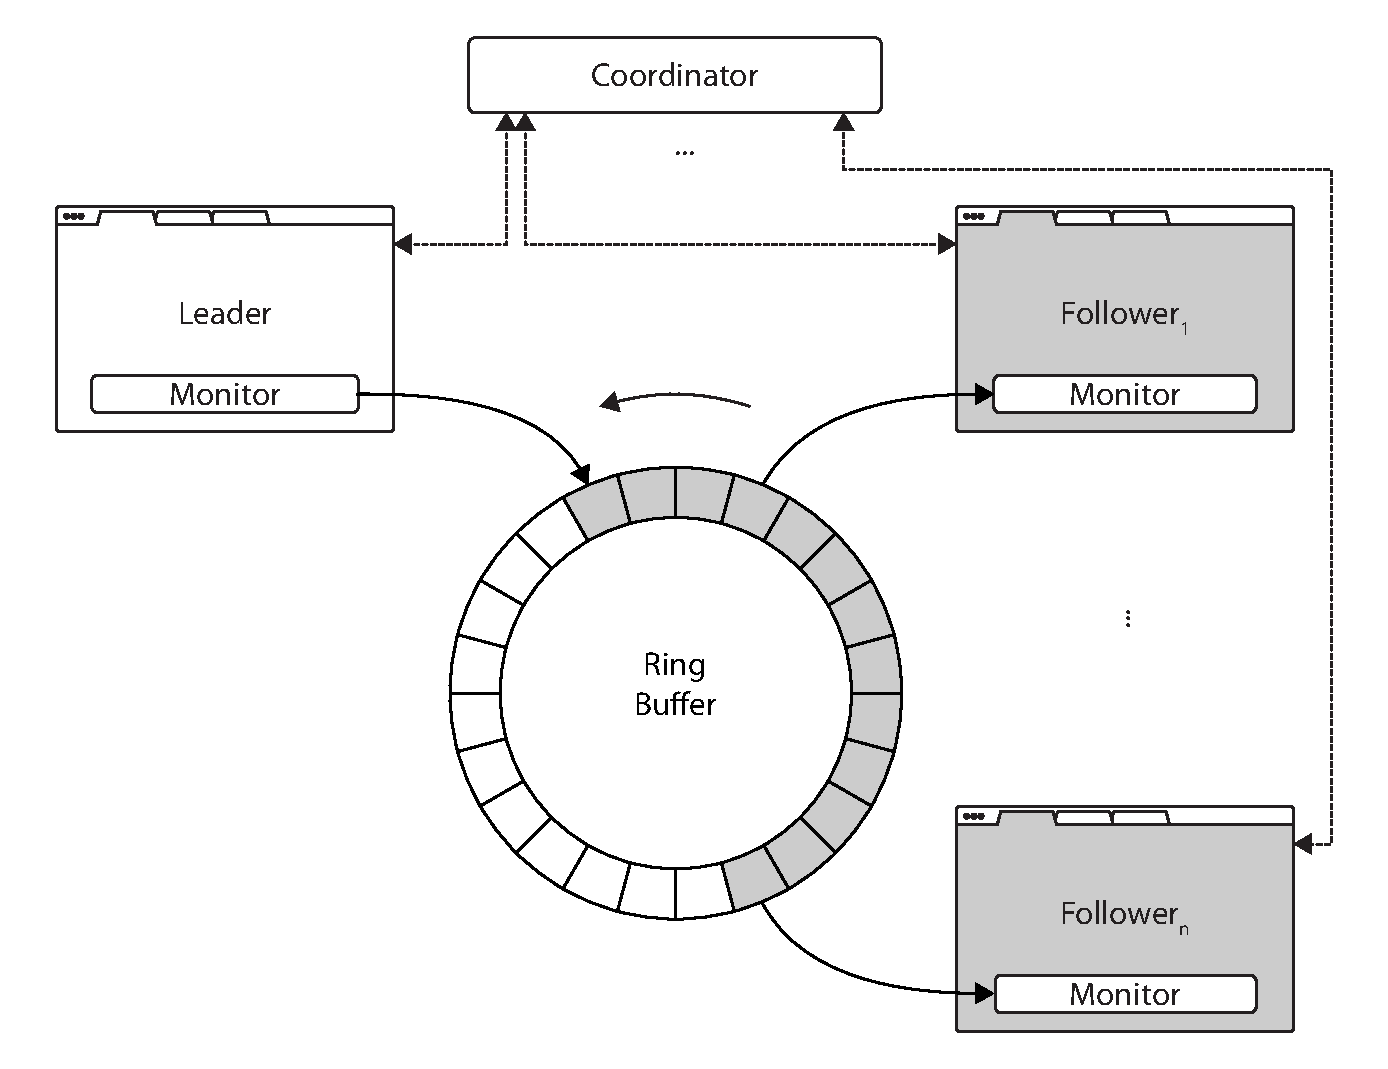
\includegraphics[width=0.6\textwidth]{efficient-execution/figures/architecture}
    \caption{The event-streaming architecture of \varan.}
    \label{fig:architecture}
  \end{center}
\end{figure}

To address these limitations, \varan uses a new approach which we call
\emph{event streaming}.  In this decentralised architecture,
depicted in Figure~\ref{fig:architecture}, one of the
versions is designated as the \textit{leader}, while the others are
\textit{followers}. During execution, the leader records all events into a
shared ring buffer, which are later read by followers to mimic the leader's
external behaviour (\S\ref{sec:streaming}). Events consist primarily
of regular system
call invocations, but also of signals, process forks (\ie \lstinline`clone`
and \lstinline`fork` system calls) and exits (\ie \lstinline`exit` and
\lstinline`exit_group` system calls).

In general, any version can be the leader, although in some situations
some may be a better choice than others--\eg when running multiple
software revisions in parallel, one might prefer to designate the
newest one as leader.  However, the leader can be easily replaced if
necessary, \eg if it crashes (\S\ref{sec:leader-repl}).

The only centralised component in this architecture is the
\textit{coordinator}, whose main job is to prepare the versions for
execution and establish the necessary communication channels.  At a
high level, the coordinator first loads the variants into memory,
injects several special handlers and memory objects into their address
spaces, rewrites any system calls in their code with jumps to the
special handlers and then starts executing the variants
(\S\ref{sec:setup}) in a decentralised manner.

%% recorded by one application version are shortly replayed
%% (\textit{streamed}) to the others, which keeps the log small, as
%% events which have been replayed by all versions can be discarded.
%% Similarly, the NVX context allows for the log to be kept in memory,
%% and for the replay to be done incrementally, with significant
%% performance advantages.  Event streaming is discussed in detail in
%% Section~\ref{sec:streaming}.


%% This is a variant of record-replay~\cite{scribe,jockey,geels06,r2},
%% but the NVX context allows us to overcome two of the main limitations
%% of traditional record-replay techniques, namely (1)~the
%% rapidly-growing log size, especially for system call-intensive
%% applications; and (2)~the long time necessary to replay the execution.
%% Because the multiple versions are executed concurrently, events
%% recorded by one application version are shortly replayed
%% (\textit{streamed}) to the others, which keeps the log small, as
%% events which have been replayed by all versions can be discarded.
%% Similarly, the NVX context allows for the log to be kept in memory,
%% and for the replay to be done incrementally, with significant
%% performance advantages.  Event streaming is discussed in detail in
%% Section~\ref{sec:streaming}.


\subsection{Rewrite rules for system call sequences}
\label{sec:rw}

In addition to eliminating the central monitor bottleneck, our
event-streaming architecture also supports (small) divergences between
the system call sequences of different variants.  For example,
different software revisions can be run inside a classical NVX
system only as long as they all issue the same sequence of system
calls~\cite{mx}.  However, software patches sometimes change the
external behavior of an application.  In particular, many divergences
in system call traces fall into the following two categories:
\begin{inparaenum}[(i)]
\item \emph{addition/removal}, characterising situations when one of
  the versions performs (or conversely does not perform) an additional
  system call, typically as a consequence of an additional check, and
\item \emph{coalescing}, covering the situations when a (repeated)
  sequence of system calls is executed a different number of times in
  each version (\eg one version might execute two \lstinline`write`
  system calls, while another version executes only one
  \lstinline`write` system call to write the same bytes because extra
  buffering is used).

\end{inparaenum}

% \begin{description}
%   \item[Addition/Removal] This class characterises situations when one
%     of the versions performs an additional system call (or conversely
%     does not perform), typically as a consequence of an additional
%     check.
%   \item[Coalescing] This class covers the situations when a (repeated)
%     sequence of system calls is executed a different number of times
%     in each version.  E.g., one version might execute two \lstinline`write`
%     system calls, while another a single equivalent \lstinline`write` to
%     write the same bytes (\eg because extra buffering is used).  
% \end{description}

\varan is the first NVX system that is able to deal with such changes.
When followers process the event sequence streamed by the leader, they
can rewrite it to account for any such differences: \eg they can skip
and merge system calls, or perform some calls themselves.  We provide
a flexible implementation of such rewrite rules using Berkeley Packet
Filters (\S\ref{sec:patternmatching}).


\section{Prototype}
\label{sec:prototype}

%% \begin{figure}[t]
%%   \begin{center}
%%     \includegraphics[width=\columnwidth]{figures/process-model}
%%     \caption{\varan process model.}
%%     \label{fig:process_model}
%%   \end{center}
%% \end{figure}

\begin{figure}[t]
  \begin{center}
    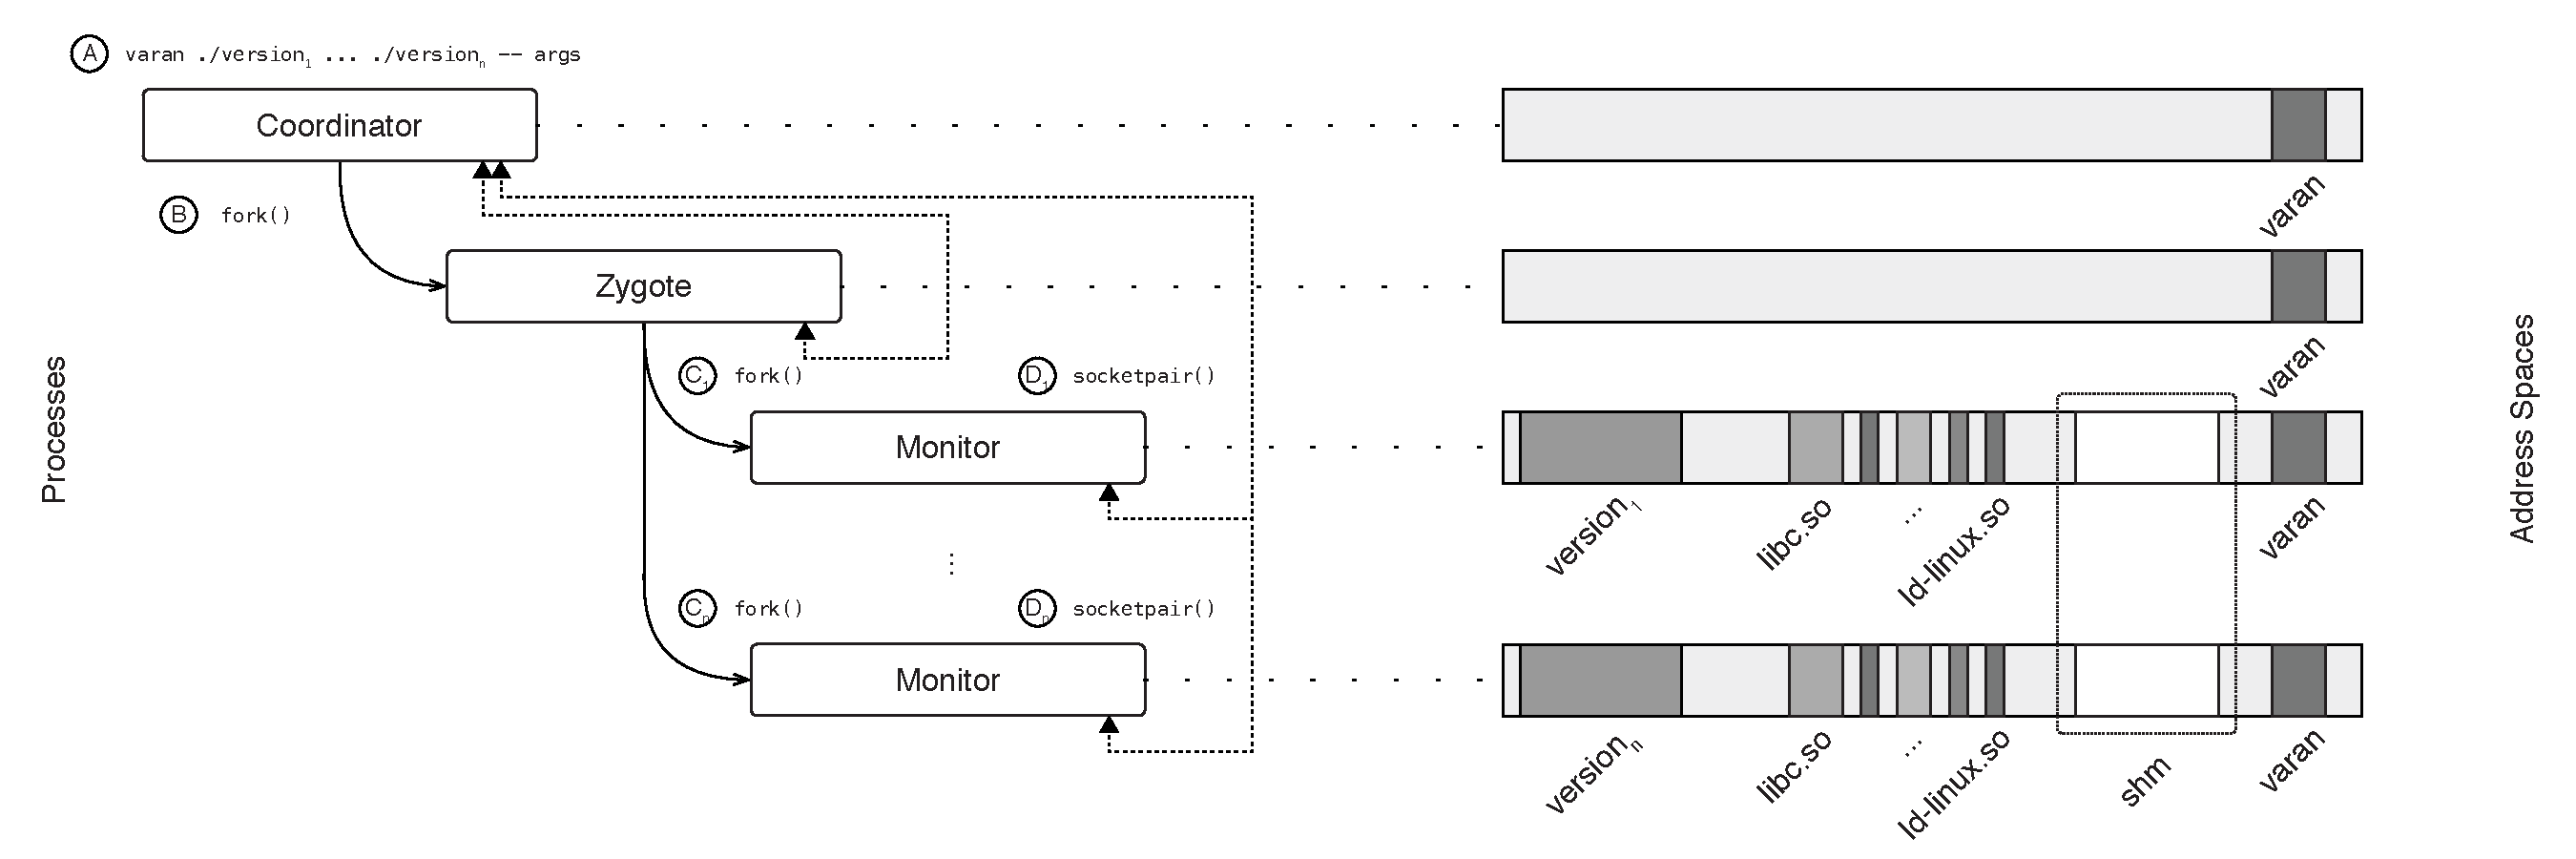
\includegraphics[width=0.75\textwidth]{efficient-execution/figures/address-space}
    \caption{Setup of address spaces and communication channels.}
    \label{fig:setup}
  \end{center}
\end{figure}


We have implemented our approach in a prototype (to which we will also
refer as \varan), targeted at multi-core processors running x86-64 Linux.
\varan works on off-the-shelf binaries (both stripped and unstripped)
and supports single- as well as multi-threaded applications.

When it starts, \varan first sets up the address spaces of all program
versions and establishes the needed communication channels
(\S\ref{sec:setup}).  It then performs selective binary rewriting to
replace all system calls with  jump instructions
(\S\ref{sec:rewriting}).  After these initial stages, the event
streamer component of \varan ensures the coordination of the leader and
its followers (\S\ref{sec:streaming}).


\subsection{Setup of address spaces and communication channels}
\label{sec:setup}

The main steps involved in the setup of version address spaces and the
needed communication channels are shown in Figure~\ref{fig:setup}.  To
run multiple versions in parallel, the user launches \varan's
\emph{coordinator} providing the paths to all versions, together with
any command line arguments required to start them (Step \circl{A} in
Figure~\ref{fig:setup}).

% \begin{lstlisting}[language=bash,numbers=none]
% varan -p /path/to/executable1 
%         -p /path/to/executable2 -- args
% \end{lstlisting}

%The coordinator is linked with the \varan library (\varanlib, stored in
%\lstinline`libvaran.so`), which will be also injected inside each version.
%\varanlib is built as a statically-linked, position-independent library,
%to make sure it does not stand in the way of any segments which have
%to be loaded by the application at fixed addresses.

The \emph{coordinator} first creates the shared memory segment
used for communication among versions, and then spawns the
\textit{zygote} process (\circl{B}), which is responsible for starting
the individual versions. The coordinator communicates with the zygote
via a UNIX domain socket. For each version $i$ that needs to be spawned,
the coordinator sends a fork request to the zygote over this socket
pair, which includes the path to that version executable, the command
line arguments, and the end-point of a socket pair which will be used
for the subsequent communication between the coordinator and that
version (\circl{C$_i$}).
%
After receiving this request, the zygote spawns a new process, which
first finalises the communication with the coordinator
(\circl{D$_i$}).  The coordinator then sends the shared memory
segment descriptor to this process, which maps it inside its address
space.

%% returns a process identifier to the coordinator.  The coordinator then
%% sends the rank and shared memory segment descriptor to the version.

In the final step, the new process starts executing inside the monitor
code, which loads the specified ELF executable and sets up the initial
address space as described in the ELF headers. If the program requires
a dynamic linker, \varan loads the linker image specified in the
header as well.
%% Afterwards, \varan attaches the shared memory segment and initialises
%% the system call table based on the rank and arguments provided by
%% the coordinator.
The text segments of both the application and the dynamic linker are
then processed by the binary rewriter (\S\ref{sec:rewriting}). Finally,
\varan jumps to the application entry point as specified in the ELF header,
starting the execution of the application version.

The right-hand side of Figure~\ref{fig:setup} shows the address spaces
of the coordinator, zygote, and program versions.  When run with
\varan, program versions have two new segments mapped into their
address spaces: the shared memory segment used for communication among
versions (``shm'') and the \varan statically-linked library
(``varan'').  Note that \varan does not prevent address-space layout
randomisation schemes to be used by the operating system.

%% \varan is operates at the thin boundary between the operating system and
%% the user-space application---\ie below the C library and the dynamic
%% linker---and lives inside the address space of the host application;
%% however, the application itself is unaware of its existence.

% The rest of this section provides some extra details regarding the
% role and implementation of the coordinator, monitor and zygote.

\boldtext{Coordinator.}  To set up the address spaces of the versions,
the coordinator acts as a specialized preloader, inspired by
\emph{rtldi}.\footnote{\url{http://www.bitwagon.com/rtldi/rtldi.html}}
However, the coordinator does not attempt to replace the existing
dynamic linker, which would be unnecessarily complex and may affect
compatibility with existing applications. Instead, it simply
intercepts the system calls performed by the linker to enable the
binary rewriter (\S\ref{sec:rewriting}) to rewrite the code of
dynamically-linked shared libraries.  One important advantage of our
interception mechanism is that we do not make use of \ptrace to
intercept calls to the dynamic linker---instead, the binary rewriter
is used to rewrite all the system calls done by the linker with jumps
into the coordinator code.  As a result, \varan can be used in
combination with existing \lstinline`ptrace`-based tools such as \gdb
or \textit{strace}, which greatly simplifies debugging.

%% This also has an advantage of supporting arbitrary dynamic linkers,
%% not just the one provided by GNU C library, albeit it is going to be
%% the most common target.

%% This architecture has several advantages over other commonly
%% approaches. \varan does not require the use of dynamic linker, as
%% required by \lstinline`LD\_PRELOAD`. 



\boldtext{Zygote.} The role of the zygote is to spawn new processes on
request from the coordinator.  Zygote processes are already used in
systems such as \textit{Android} and
\textit{Chrome}~\cite{linuxzygote}---in this paper, we use the term to
refer to the architectural pattern rather than a particular implementation, as \varan
provides its own clean-slate implementation.  While it would be
technically possible for the coordinator to create the processes in
which versions run, this would bring some complications regarding the
communication channels: for example, the second version spawned would
inherit the communication channel between the first version and the
coordinator, which would be undesirable.

\boldtext{Monitor.} The monitor code is built as a statically-linked,
position-independent library, to make sure it does not stand in the
way of any segments which have to be loaded by the application at
fixed addresses.  To ensure that the code can be compiled like this,
we must avoid using any global variables (\ie those in the
\lstinline`.data` section). One consequence is that \varan
cannot use any of the existing C libraries such as \textit{GNU C
  Library}, as these are not typically built to support this
requirement.  Instead, \varan provides its own implementation of the
necessary C library functions based on the \textit{Bionic C
  library}.\footnote{\url{https://android.googlesource.com/platform/bionic}}
To support the use of Linux system calls, \varan uses a modified
version of the \lstinline`linux_syscall_support.h`
header.\footnote{\url{https://code.google.com/p/linux-syscall-support/}}

%% \varanlib provides its own entry point (\ie the \lstinline`\_start` function),
%% which is the starting point for \varan's execution. After start, it first
%% processes the arguments passed on stack by the Linux kernel, including
%% program arguments, environment variables and most importantly the
%% auxiliary data. Then, it loads the specified ELF executable into the
%% address space. Since \varan operates as a pre-loader, it is responsible
%% for setting up the initial address space layout as described by the
%% program header. If the program being executed requires dynamic linker,
%% \varan loads the linker image specified in the program header as
%% well. The text segments of both the application and the dynamic linker
%% are then processed by the binary rewriter (\S\ref{sec:rewriting}).


%% After start, \varan sets up the communication subsystem (\ie the shared
%% memory allocator, the ring buffer) and then forks the Zygote
%% process. The Zygote closes all open descriptors except for the socket
%% used as a communication channel with the coordinator and enters the
%% dispatch loop to wait for incoming requests. On fork request, the
%% Zygote receives command line arguments (\ie \lstinline`argv`) and a set of
%% file descriptors which will be available to the new process; then
%% forks itself and resumes to dispatch loop. The other type of requests
%% that Zygote supports are querying for process status (\ie equivalent
%% of \lstinline`waitpid`) and process termination (\ie \lstinline`SIGKILL`).

%% \begin{structure}
%% \item Establishing the initial memory layout as specified by the ELF
%% binary
%% \item Loading the dynamic loader (if specified by the ELF header)
%% \item Jumping to the application (or dynamic loader) entry point
%% \end{structure}


\subsection{Binary Rewriting}
\label{sec:rewriting}

%% \begin{structure}
%% \item Scanning each text segment in the program address space
%% \item Rewriting every syscall with jump instruction where possible,
%% otherwise using interrupt
%% \item Using table of system call handlers to interpose on selected
%% system calls
%% \end{structure}

To intercept system calls, \varan uses selective binary
rewriting~\cite{bird}. Unlike traditional dynamic binary rewriting
implemented by tools like DynamoRIO~\cite{dynamorio02} or
Pin~\cite{pin05}, where the entire process image is being rewritten,
often introducing a significant performance overhead, \varan only
replaces the instructions for performing system calls (\ie
\lstinline[language={[x64]Assembler}]`int $0x80` on x86 and
\lstinline[language={[x64]Assembler}]`syscall` on x86-64).
%% This approach has been originally implemented in
%% \emph{BIRD}~\cite{bird} for the Windows/x86 platform and later in
%% \emph{seccompsandbox}\footnote{\url{https://code.google.com/p/seccompsandbox/}}
%% for Linux. 
%Our implementation extends the \emph{seccompsandbox}\footnote{\url{https://code.google.com/p/seccompsandbox/}} framework for Linux.

The rewriting itself is done when a segment is mapped into memory with
executable permissions, or an existing memory segment is marked as
executable.  
%(\ie \lstinline`mmap` system calls with executable flag, typically
%performed by the dynamic linker).
During rewriting, \varan scans the segment searching for system call
instructions using a simple x86 disassembler.  Every system call found
is rewritten with a jump to an internal system call entry point. This
process is complicated by the fact that while a system call
instruction is only one byte long, a jump instruction requires five
bytes.  Therefore, in order to rewrite the system call with a jump, we
also need to relocate some of the instructions surrounding the system
call---\ie perform binary detouring via trampolines~\cite{detours}.
On the rare occasions when this is not possible (\eg because the
surrounding instructions are potential branch targets), we replace the
system call with an interrupt (\lstinline`INT 0x0`).  This interrupt
is handled by \varan through a signal handler installed during
initialisation, which redirects the control flow to the system call
entry point as for other system calls.

The system call entry point first saves all registers, and then
consults an internal system call table to check whether there is a
handler installed for that particular system call; if so, it calls
that handler, otherwise it invokes the default handler.  After
processing the system call, the entry point handler restores all
registers and returns to the original caller (using
\lstinline`sigreturn` in the case of system calls intercepted via an
interrupt). The system call entry point also implements support for
restarting system calls (\ie signaled by the \lstinline`-ERESTARTSYS`
error code). This is used in certain scenarios supported by \varan
such as transparent failover (\S\ref{sec:failover}).

The internal system call table can be easily changed to accommodate
various application scenarios.  In particular, the only difference
between the leader and the followers is the system call table. For
example, the \lstinline`write` system call would be redirected in the leader
to a function that performs the call and records its result in the
shared ring buffer, while in the followers it would be redirected to a
function that reads the results from the shared buffer without making
the call.
%% \varan allows both the system call table and the default system call
%% handler to be provided by the embedder of \varan \todo{Where shall we
%%   described the possibility of \varan embedding, \ie building tools on
%%   top of \varan?}. This makes it easy to customize \varan behavior for
%% different use cases (\S\ref{sec:failover}). For our prototype, we have
%% provide three different system call tables (\ie record, replay and
%% passthrough). 
\varan  also provides a Python script which can produce new tables
and their implementations using templates.
%% ; in fact, the passthrough table was implemented using this
%% generator. We have also used the generator throughout the \varan
%% development for testing and debugging purposes.

Finally, note that in order to prevent potential attackers to easily inject
system calls into the program, the binary rewriter follows a
W$\mathbin{\oplus}$X discipline throughout execution, making sure that
segments are not marked as both writable and executable at the same
time.


\subsubsection{Virtual System Calls}
\label{sec:vsyscall}

Certain Linux system calls are accelerated through the \emph{vsyscall}
page and the \emph{vDSO} segment. These are mapped into the address
space of each Linux process, and contain system call
implementations. These \textit{virtual system calls} do not incur the
context switch overhead between kernel and user space associated with
standard system calls.

The \emph{vsyscall} page was introduced first, but is being deprecated
in favor of the \emph{vDSO} segment.
%% limitations\footnote{We are referring to x86-64 version, on x86
%%   systems the vDSO segment contains a function used to determine the
%%   preferred method of making a system call}. 
The main reason for this development is that the \emph{vsyscall} page
is mapped to a fixed address, making it susceptible to return-oriented
programming attacks~\cite{ROP:tissec12}. To address this issue, the
vDSO segment is mapped to a random address. Since the segment is
dynamically allocated, it can also support an arbitrary number of
virtual system calls (currently \lstinline`clock_gettime`, \lstinline`getcpu`,
\lstinline`gettimeofday` and \lstinline`time`).

Virtual system calls represents one of the major limitations of
\lstinline`ptrace`-based monitors. Since these system calls are entirely
implemented in user space, they cannot be intercepted via \ptrace.
This is an important limitation: as these system calls provide access
to timing information, they are often used as a source of
non-determinism (\eg for random number generators) and their handling
is critical for any NVX system. %Despite this, previous systems either
%omit discussion on virtual system call handling~\cite{mx,orchestra11}
%or explicitly mention their inability to handle them~\cite{tachyon12}.

To our knowledge, \varan is the first NVX system which handles virtual
system calls, using binary rewriting. 
%In \varan, binary rewriting is also used to intercept virtual system
%calls.
Handling calls made via the \textit{vsyscall} page is easier because
the function symbols are always mapped to the same address.  
%% We can therefore easily identify calls to these functions while
%% scanning the text segment and rewrite them to calls into our system
%% call table.
To handle \textit{vDSO} calls, we first need to determine the base
address of the \textit{vDSO} segment; this address is passed by the
kernel in the ELF auxiliary vector via the \lstinline`AT_SYSINFO_EHDR`
flag.\footnote{\url{https://www.gnu.org/software/libc/manual/html_node/Auxiliary-Vector.html}}
Second, we need to examine the ELF headers of the \textit{vDSO}
segment to find all symbols.  Identifying calls to these symbols is
more complicated than in the \textit{vsyscall} case because these
symbols are allocated at arbitrary addresses.  Instead, we replace the
entry point of each function with a jump to dynamically generated code
which sets up the stack and then issues a call to the \varan system
call entry point as in the case of regular system calls. Furthermore, we
provide a trampoline, which allows the invocation of the original
function, by moving the first few instructions of each function to a
new place, followed by a jump to the original code. This allows \varan
to take advantage of the virtual system call mechanism to further
improve performance.

%% Finally, we note that this function interception mechanism is not
%% specific to system calls and can be used to intercept arbitrary
%% functions in the target application if needed, similarly to
%% Detours~\cite{detours}.



\subsection{Event Streaming}
\label{sec:streaming}

%% \begin{structure}
%% \item Externally observable behavior triggers events (\eg system calls,
%% signals), these events are being recorded and replayed by individual
%% versions
%% \item The concept of event-streaming; all versions share a common event
%% stream (\ie log) of fixed size
%% \item One version is always elected as a leader adding new events to the
%% stream, the other versions are followers replaying the events from the
%% stream
%% \item When the leader crashes, followers elect a new leader
%% \end{structure}

As we discussed briefly in Section~\ref{sec:overview} and illustrated
graphically in Figure~\ref{fig:architecture}, the leader records all
external events into a shared ring buffer, while the followers replay
them to mimic the leader's behavior. The leader is the only version
interacting with the environment, \ie executing the system calls, with
the exception of system calls which are local to the process (\eg
\lstinline`mmap`). % or \lstinline`sigaction`).

As in any NVX system operating at the level of system calls, \varan
has to be aware of the system call semantics, in order to transfer the
arguments and results of each system call.  \varan currently
implements \syscallsHandlers system calls, which were all the system
calls encountered across our benchmarks.\footnote{We configured \varan
  to emit an error message when an unhandled system call is
  encountered, and have implemented system call handlers on demand.}

%% All application instances running in parallel under \varan are assigned
%% ranks, similarly to OpenMPI~\cite{OpenMPI}. The instance\footnote{We
%%   refer to the instances rather than a process as application may have
%%   multiple threads/subprocesses} with rank 0 is denoted as
%% \emph{leader} while all other instances are denoted as
%% \emph{followers}. 


%% When followers would execute a system call under normal execution, now
%% they simply return a value from the event stream (\ie the return value
%% of the system call executed by the leader).

% \varan recognizes several different types of events:
% \begin{inparaenum}[(i)]
% \item \emph{syscall} for the system call entry,
% \item \emph{sysret} for the system call exit,
% \item \emph{signal} for an interceptable signal,
% \item \emph{exit} for the process exit.
% \end{inparaenum}
% Furthermore, it is possible to add other types of events if necessary.

%% Each event has a fixed size of 64 bytes where first byte is
%% used as an event type.  The size has been deliberately chosen to be
%% fit into a single cache line on modern x86 CPU (see \S\ref{sec:ipc}
%% for more details).

%% \subsection{Interprocess Communication}
%% \label{sec:ipc}

%% \begin{structure}
%% \item Sending events from one process to other without the use of system
%% calls to avoid the additional overhead
%% \item Shared memory queues for process to process communication
%% \item Custom shared memory allocator with reference counting
%% \end{structure}

%% Since one of our primary goals for \varan was to minimize the performance
%% overhead, to avoid additional system calls being made during system
%% call handling (\S\ref{sec:overview}), we have designed an interprocess
%% communication mechanism which does not use system calls (\eg
%% socket-based communication primitives).

\subsubsection{Shared ring buffer}
\label{sec:ring}

For fast communication, the leader and its followers share a common
ring buffer of fixed size, which is held entirely in memory.  Our
initial solution used a separate shared queue for each
process~\cite{fastforward,mcringbuffer}, with the
%% Shared memory queues are often used for fast core-to-core
%% communication in high-performance applications.
coordinator acting as an event pump---reading events from the leader's
queue and dispatching them into followers' queues.  This approach
worked well for a low system call rate, but at higher rates the event
pump quickly became a bottleneck.  
% Furthermore, although we used a
% state-of-the-art shared queue implementation~\cite{bqueue}, we still
% experienced a large performance overhead for system call
% interception---over $20\times$ for a worst-case microbenchmark,
% compared to $4\times$ in the final implementation.

As a result, we have instead opted for a design based on the Disruptor
pattern~\cite{disruptor}, which uses a shared ring buffer allowing concurrent
access by multiple producers and consumers, eliminating the need to dispatch
events among queues, and thus improving both performance and memory
consumption.  Our implementation uses C11 atomics, 
%introduced in C11 and now supported by both GCC and Clang, 
in combination with cache aligning to
achieve maximum performance with minimal use of locking (locks are used only
during memory allocation and deallocation).

%The ring buffer is used to stream events between processes.  
The size of the ring \varan uses is configurable and has a default
value of 256 events.  Each event has a fixed size of 64 bytes; the
size has been deliberately chosen to fit into a single cache line on
modern x86 CPUs.  This is sufficient for sending signals and system
calls for which all arguments are passed by value (on x86-64, a system
call can have up to six arguments of eight bytes, to fit into general
purpose registers).  However, for system call arguments passed by
reference, the payload might have variable size and can be potentially
larger than the event itself.  In this case, we use events only to
transfer shared pointers, which identify memory shared across
versions.

The use of a shared memory buffer may result in a waste of system
resources when the leader process performs a system call which blocks
for a long period of time, as the followers use busy waiting to check
for new events. To address this problem, we have introduced the
concept of a \emph{waitlock}. Whenever a follower makes a blocking
system call, it acquires the waitlock. If there is no event available,
the thread will block until the leader wakes up and notifies it. The
waitlocks are efficiently implemented using a combination of C11
atomics and futexes~\cite{futex}.

\subsubsection{Transferring file descriptors and leader replacement}
\label{sec:leader-repl}

Apart from the ring buffer, each version has a \textit{data channel},
implemented using UNIX domain sockets.
% Together, the ring buffer and data channel form an \emph{event
% stream} which is a primary communication mechanism for exchanging
% events among instances.
The data channel is used to send information which cannot be
transferred via shared memory, in particular open file descriptors.
Whenever the leader obtains a new file descriptor (\eg by opening a
file), it sends this descriptor to all followers, effectively
duplicating the descriptor into their processes. This is a crucial
mechanism which enables the leader to be replaced transparently when
it crashes. When the leader crashes, the follower that is elected as
the new leader can simply continue executing using existing
descriptors (\eg responding to requests coming over the network)
without any disruption of service.

% Currently, UNIX domain sockets do not support broadcast, so the leader
% communicates with the followers via the coordinator, which then sends
% the descriptor separately to all followers.  However, there are
% proposals to add broadcast support for UNIX domain
% sockets,\footnote{\url{https://lkml.org/lkml/2012/2/20/208}} which would
% simplify the design of our prototype and further improve performance.


\subsubsection{Multi-process and multi-threaded applications}
\label{sec:threading}
\label{sec:ipc}

Handling processes and threads is crucial in supporting many modern
applications.  
%The discussion below refers to processes, but threads are handled in a
%similar way.
In our design, we have opted to have separate ring buffers for each
tuple of processes or threads in the system: for instance, when a
process forks, the parent processes in the leader and all followers
form one tuple, and the child processes another, with a process in
each tuple acting as the leader.  More exactly, when a new process is
forked, a new socket pair is established between the process and the
coordinator and a new ring buffer is allocated.  The leader then
continues execution, but the coordinator waits until all followers
fork a new process, establishing appropriate socket pairs for
communication, and setting the child processes to read events from the
newly-allocated ring buffer.

To alleviate non-determinism issues due to scheduling, \varan enforces
system call ordering across all tuples using Lamport's
\emph{happens-before} relation~\cite{lamport78}. Currently, this is
only implemented for multi-threaded applications, which make intensive
use of synchronisation primitives, but the same solution could be
employed for multi-process applications too.

\begin{figure}[t]
  \begin{center}
    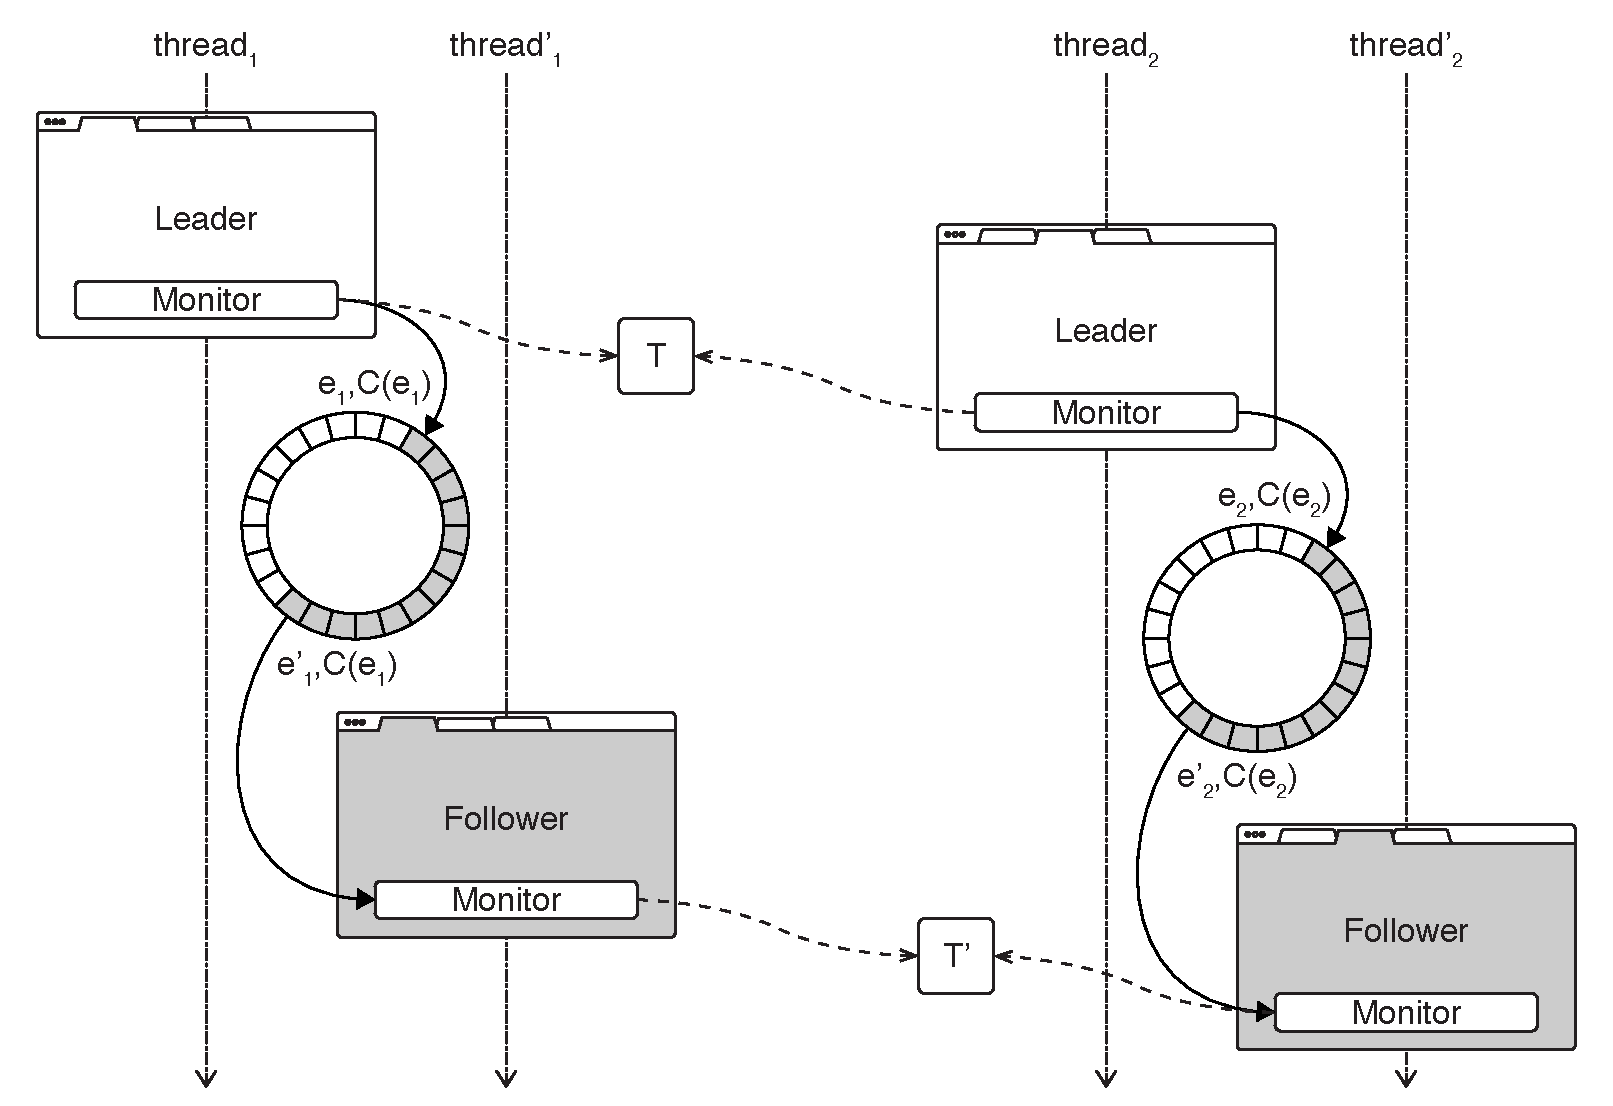
\includegraphics[width=0.75\textwidth]{efficient-execution/figures/multithreading}
    \caption{Event delivery in a multi-threaded NVX program, with
      the ordering of events enforced using logical clocks.}
    \label{fig:multithreaded}
  \end{center}
\end{figure}

Each variant has an internal Lamport clock, shared by all threads, and
each event $e_i$ sent through the ring buffer is annotated with a
timestamp $C(e_i)$.  Then, when replaying events from the buffer, each
thread checks the timestamp of every new event and only receives the
event if it does not violate the happens-before relation. This
scenario is depicted in Figure~\ref{fig:multithreaded}. If $e_1\to
e_2$ ($e_1$ happens before $e_2$), then $C(e_1)<C(e_2)$ and \varan
enforces $e'_1\to e'_2$. Without the ordering, there could be a
situation where $e_1\to e_2$, but $e'_1\not\to e'_2$, which could lead
to a divergence. A similar approach has been proposed in the past for
record-replay in shared-memory systems~\cite{levrouw94}.

To implement the internal clocks shared by the threads of a variant
($T$ and $T'$ in Figure~\ref{fig:multithreaded}),
we use an atomic counter allocated in the shared memory space and
updated using C11 atomics for efficiency.  When the leader thread
writes a new event into the ring buffer, it increments its variant's
clock value and attaches it to the event.  When a follower thread
reads an event from the ring buffer, it compares its variant's clock
value with the event's timestamp.  If they are equal, the thread
increments its variant's clock value and processes the event,
otherwise it continues waiting. Our current implementation uses busy
waiting, as the wait times are expected to be small.  However, shall
this become a problem in the future, it is possible to use blocking
wait instead (\eg a futex).

% Since Disruptor (\S\ref{sec:ring})
% allows concurrent writes by multiple producers without the need for
% expensive synchronisation, the use of a single shared buffer does not
% create a performance bottleneck. %hinder the application performance.

Our solution resembles existing deterministic multi-threading (DMT)
mechanisms~\cite{coredet:asplos10,dthreads:sosp11}. The guarantees
provided by \varan are weaker than those typically provided by these
systems as we do not enforce ordering across atomics-based
synchronisation primitives. We have not detected any system call
divergences caused by related data races in our benchmarks, which
include multi-threaded applications (\eg \redis), similar to the
experience reported for prior NVX systems. However, shall this become
a problem, we could address it by employing a stronger form of
determinism similar to existing DMT systems.

%
% However, this weaker form of determinism
% does not typically pose a problem for real-world applications as long
% as they are properly synchronised.  Note that data races resulting
% from missing or incorrect synchronisation can cause followers to issue
% a different sequence of system calls from the leader.  If this
% happens, we could either try to apply one of the rewriting rules
% (\S\ref{sec:patternmatching}), or terminate the follower.
%

%% Each instance also has a dedicated \emph{service channel}, similarly
%% to the data channel implemented using UNIX domain sockets. The service
%% channel is used to transfer commands and service requests between
%% coordinator and the instance.

%% One such example are \lstinline`fork` and \lstinline`clone` system calls. The new
%% process spawned as a result of these system calls needs to have its
%% own data and service channel. The parent process is responsible for
%% creating these using a \lstinline`sockepair` system call. One end of each
%% pair is inherited by the new process while the other end is sent to
%% the coordinator where it is associated with the new process.

%Note that data races resulting from missing or incorrect
%synchronisation can cause followers to issue a different sequence of
%system calls from the leader.  If this happens, that follower would
%have to be terminated.  We first note that \varan has not detected any
%system call divergences caused by data races in our benchmarks (which
%include many popular applications such as \apache, \nginx, and \redis),
%so this might not be such an important aspect in practice.  Prior NVX
%systems do not address this problem either, likely due to a comparable
%experience.

%However, we envision two possible solutions.  The first one would be
%to use deterministic multi-threading (\eg
%Dthreads~\cite{dthreads:sosp11}).  The second solution would be to
%allow developers to document any benign races as rewrite rules
%(cf. \S\ref{sec:patternmatching}).

\subsubsection{Memory allocation scheme}  

Efficient shared memory allocation plays an important role in a system
like \varan.  We use a custom shared memory pool allocator implementation.
%, similar to the one used by OpenMPI.\footnote{\url{http://www.open-mpi.org/}}
The allocator has the notion of buckets for different allocation sizes,
where each bucket holds a list of segments, and each segment is
divided into chunks of the same size; each bucket holds a free list of
chunks.  When there are no more unused chunks in a bucket, the
allocator requests a new segment from the memory pool, and divides it
into chunks which are then added to the free list. Each bucket also
has a lock associated with it which has to be held prior to an
allocation from that bucket. 
% While this design is relatively simple,
% it performed well in our benchmarks. We also experimented with
% more advanced designs (\eg using different allocation strategies for
% smaller and larger blocks), but the basic allocator always
% outperformed all other implementations.  

%% However, we believe it might still be possible to come with a more
%% specialized allocation strategy which would further improve the
%% performance of \varan, and this is something we would like to address in
%% our future work.

%% The critical part of many systems which use shared memory for
%% communication is deallocation. There are various solutions to this
%% problem. One possibility is to use some form of garbage collection,
%% such as reference counting. Unfortunately, this solution is not
%% applicable in our case since the leader is not aware of any of the
%% consumers processing its events making it difficult to consistently
%% manage the reference counts. The original Disruptor implementation,
%% which targets the Java runtime simply relied on the garbage collector
%% provided by the virtual machine. Unfortunately, this solution is not
%% applicable in our case either. Instead, we have extended the C-based
%% Disruptor implementation to notify a follower if it is the last one
%% that processes an event. \todo{how?}  If that is the case, the
%% follower is responsible for freeing the associated memory. This
%% solution does not add any overhead and does not require any
%% modifications to the allocator.

% This property allows us sharing memory between individual application
% instances without explicitly tracking which instance is responsible for
% deallocation, or using the back channel to notify instance that the block is
% available for deallocation as in the case of OpenMPI

\subsection{Rewrite rules for system call sequences}
%\subsubsection{System call filtering and rewriting}
\label{sec:patternmatching}

\varan uses Berkeley Packet Filters (BPF)~\cite{bpf} to implement the system call
rewrite rules introduced in Section~\ref{sec:rw}.  BPF is a machine
language for writing rules and an interpreter shipped with many UNIX
implementations, including Linux and BSD.  BPF filters have been
traditionally used to filter network packets, but recently also for
system call filtering as a part of seccomp ``mode 2'' (also known as
seccomp-bpf).

We have integrated a BPF interpreter in \varan to allow for system
call rewrite rules. Our implementation is based on the Linux kernel
code which was ported to user space and extended for NVX
execution. \varan provides BPF extensions on top of the instruction
set used by seccomp-bpf.\footnote{\url{https://www.kernel.org/doc/Documentation/networking/filter.txt}}
The \lstinline[language={[bpf]Assembler}]`event` extension allows
access to the event stream, which can be used to compare the system
calls executed across versions, as we will show in
Section~\ref{sec:mv-execution}.

%We have also made the offset, used to access the \lstinline`struct seccomp_data` content writable.

% This required adding a new return value
% \lstinline`SECCOMP_RET_REPLACE` where the bottom 16-bits of the return
% value specify the new system call number the original system call is
% going to be rewritten to.  Since these extensions does not add any new
% instructions or extend the semantics of the BPF language, the
% \lstinline`bpf_asm` tool can be used to compile the filters into a
% binary form. This can be then loaded into \varan on start through a
% command line option.


The use of BPF has a number of advantages.  First, it does not require
the user to modify and recompile the monitor on every rule
change. This is particularly important as rewrite rules can be
application specific. Second, the BPF machine language was designed to
be simple enough to prevent certain classes of errors---in particular,
all filters are statically verified when loaded to ensure termination.
% (\ie every filter has to end with a \lstinline`ret` instruction).



%We also argue that the choice of BPF as a language for stream rewriting rules
%makes it easier to adopt by administrators, the most likely users of \varan,
%compared to some other more esoteric languages such as Haskell~\cite{tachyon}.

%% \begin{lstlisting}{language=[bpf]Assembler,caption={Example of a BPF rewriting rule}}
%% ld [0]                /* offsetof(struct seccomp_data, nr) */
%% jne #1, good          /* __NR_write */
%% bad: ret #0           /* SECCOMP_RET_KILL */
%% ldi #18               /* __NR_pwrite */
%% add #0x00070000       /* 18 + 0x00070000 */
%% ret %a                /* SECCOMP_RET_REWRITE */
%% good: ret #0x7fff0000 /* SECCOMP_RET_ALLOW */
%% \end{lstlisting}

\section{Performance evaluation}
\label{sec:evaluation}

One of the main contributions of \varan is a significantly lower
performance overhead compared to existing state-of-the-art NVX
systems.  Therefore, we have conducted an extensive performance
evaluation, using microbenchmarks (\S\ref{sec:microbenchmarks}),
high-performance C10k servers (\S\ref{sec:c10k}) and applications used to
evaluate prior NVX systems (\S\ref{sec:comparison}).

The benchmarks were run on a four-core/eight-thread machine with
a 3.50~GHz Intel Xeon~E3-1280 CPU and 16~GB RAM running 64-bit Ubuntu 14.04
LTS. Both the server and client application on the same machine using the
loopback device to ensure that CPU is fully saturated.
%while the servers were run on a pair of such machines, one
%running the server under \varan and the other the client.  The machines are
%located in the same rack, connected by a 1~Gb Ethernet link.

\subsection{Microbenchmarks}
\label{sec:microbenchmarks}

To measure the overhead introduced by \varan while processing individual
system calls, we designed a series of experiments that compare a
system call intercepted and executed by \varan against the same system
call executed natively. We used five different system calls:

\begin{enumerate}

%\item \lstinline`close` is representative of an inexpensive system call.
%  We invoke it with argument \lstinline`-1`, which returns immediately
%  with an error representing a NOP system call.

\item \lstinline`close(-1)` is representative of an inexpensive system call,
  which returns immediately.

%\item \lstinline`write` is representative of system calls which involve
%  expensive I/O, but whose result can be sent entirely as a single
%  event in the ring buffer.  We invoke the system call to write a
%  512-byte buffer to \lstinline`/dev/null`.

\item \lstinline`write(DEV_NULL, "...", 512)` is representative of system
  calls which involve expensive I/O, but whose result can be sent
  entirely as a single event in the ring buffer.

%\item \lstinline`read` is representative of system calls which involve
%  expensive I/O, and whose result cannot be fully included in the
%  associated event in the ring buffer.  Instead, it has to be copied
%  via additional shared memory (\S\ref{sec:ring}). We invoke the
%  system call to read a 512-byte buffer from \lstinline`/dev/zero`.

\item \lstinline`read(DEV_NULL, "...", 512)` is representative of system calls which
  involve expensive I/O, and whose result cannot be fully included in the
  associated event in the ring buffer.  Instead, it has to be copied via
  additional shared memory (\S\ref{sec:ring}).

%\item \lstinline`open` is representative of system calls that require
%  transferring file descriptors (\S\ref{sec:leader-repl}).  We invoke
%  it with \lstinline`/dev/null` and \lstinline`O\_RDONLY` as arguments.

\item \lstinline`open("/dev/null", O_RDONLY)` is representative of system calls that
  require transferring file descriptors (\S\ref{sec:leader-repl}).

\item \lstinline`time(NULL)` is a virtual system call implemented via the
  \textit{vDSO} segment (\S\ref{sec:vsyscall}). It internally calls
  \lstinline`__vdso_time` (since glibc 2.15).  We could not measure
  the overhead of using the \textit{vsyscall} page, because it is
  deprecated on our system (and all recent versions of Linux), with
  all \textit{vsyscalls} now redirected to their \textit{syscall}
  versions.

\end{enumerate}

%% The \lstinline`open` demonstrates the cost of the file descriptor transfer; we have
%% used the \lstinline`/dev/null` file with \lstinline`O\_RDONLY` flag. \lstinline`read` and
%% \lstinline`write` use the I/O performance overhead, by reading and writing 512B
%% buffer from \lstinline`/dev/zero` and to \lstinline`/dev/null` respectively. The \lstinline`read`
%% is clearly more expensive system call, as it needs to transfer the content of
%% the buffer read using the shared memory (\S\ref{sec:streaming}). The
%% \lstinline`close` system call is a representative of all other cases.

We execute each system call one million times and compute the average
of all execution times.  Time measurements were done using the time
stamp counter (\ie the \lstinline`RDTSC` instruction). Each set of
measurements was preceded by a warm-up stage in which we executed the
system call \num{10000} times. % to warm up the caches.

\begin{figure}[!t]
  \centering
  \includegraphics[width=\textwidth]{efficient-execution/graphs/micro}
  \caption{System call microbenchmarks.}
  \label{fig:micro_syscall}
\end{figure}

%\begin{figure}[!t]
%  \centering
%  \includegraphics[width=\columnwidth]{results/micro_syscall}
%  \caption{System call microbenchmarks.}
%  \label{fig:micro_syscall}
%\end{figure}

Figure~\ref{fig:micro_syscall} shows the results.  The first set of
bars labeled \textit{native} shows the execution time without \varan.
The second set of bars labeled \textit{intercept} shows the execution
time with interception, measuring the cost of binary rewriting: for
these experiments, the intercepted system call is immediately
executed, without any additional processing.  As it can be seen, the
interception cost is small, at under \maxInterceptOvh in all
cases. The overhead of intercepting the virtual system calls is high
in relative terms, but low in absolute ones: \vdsoIntercept vs
\vdsoNative for native execution in case of \lstinline`time`.

The set of bars labeled \textit{leader} shows the execution time for
each system call to be intercepted, executed and recorded by the
leader.  That is, it is the sum of the \textit{intercept} cost and the
cost of recording the system call.  For \lstinline`close` and \lstinline`write`,
the overhead is only \closeLeaderOvh and \writeLeaderOvh respectively
on top of the native execution, because the arguments and results of
these system calls can be recorded in a single event.  For \lstinline`read`,
this is more expensive, at \SI{139}{\percent}, because transferring the result also
involves accessing additional shared memory.  Finally, the cost for
\lstinline`open` is the highest, since it also involves the slower transfer
of the returned file descriptor via a UNIX domain socket.

Finally, the set of bars labelled \textit{follower} shows the execution
time of the follower, which has to intercept each system call and read
its results from the ring buffer and (if necessary) shared memory.  As
expected, the costs for \lstinline`close` and \lstinline`write` are low (and
significantly lower than executing the system call), because the
entire result fits into a single event on the ring buffer. The costs
for \lstinline`read` and \lstinline`open` are higher, because they involve
additional shared memory and transferring a file descriptor,
respectively, but they are still lower than the costs incurred by the
leader.


%\boldtext{vDSO calls.}  We similarly measured the overhead of
%performing a virtual system call via the \textit{vDSO} segment
%(\S\ref{sec:vsyscall}).  The system call used was \lstinline`time`,
%which internally calls \lstinline`\_\_vdso\_time` (since \stt{glibc
%  2.15}).  We could not measure the overhead of using the
%\textit{vsyscall} page, because it is deprecated on our system (and
%all recent versions of Linux), with all \textit{vsyscalls} now
%redirected to their \textit{syscall} versions.

%\begin{figure}[!t]
%  \centering
%  \includegraphics[width=\columnwidth]{results/micro_vsyscall}
%  \caption{vsyscall and vDSO microbenchmarks.}
%  \label{fig:micro_vsyscall}
%\end{figure}

%Figure~\ref{fig:micro_syscall} shows the results, using the same set
%of bars as in Figure~\ref{fig:micro_syscall}.  We have opted this time
%to show absolute numbers, and to include the data for \lstinline`close(-1)`
%from Figure~\ref{fig:micro_syscall} for comparison.  The overhead of
%intercepting the system call is high in relative terms, but low in
%absolute ones: \vdsoIntercept vs \vdsoNative for native execution.
%The \textit{leader} and \textit{follower} costs are similarly high in
%relative terms but low in absolute ones: \vdsoLeader and
%\vdsoFollower, respectively.

\subsection{C10k servers}
\label{sec:c10k}

Existing NVX systems, including those based on \stt{ptrace}, can already
run CPU-bound applications efficiently with overhead typically $<20\%$.
As a result, we focus our evaluation on high-performance, heavily
I/O-bound C10k servers which%
\begin{inparaenum}[(1)]
\item represent the worst-case scenario for a system-call monitor; and
\item form the backbone of modern, highly-scalable web applications, for
  which security and availability are critical.
\end{inparaenum}

The \nservers server applications used in our evaluations are
summarized in Table~\ref{tbl:apps} (the size is measured in lines of
code, as reported by the \stt{cloc} tool). For our performance experiments, we
ran the same version of each application multiple times with different number
of instances (in practice you would typically run different versions). Each
experiment was performed six times, with the first measurement used to warm up
the caches and discarded.  The overhead was calculated as a median of the
remaining five measurements.

\begin{table}
  \centering
\begin{tabular}{lcrl}
  \toprule
  \textsc{Application} & \textsc{Size} & \textsc{Threading} \\
  \midrule
  Beanstalkd & 6,365 & single-threaded \\
  Lighttpd & 38,590 & single-threaded\\
  % Memcached & 9,779 &  multi-threaded\\
  % MongoDB & 898,293 & multi-threaded \\
  Nginx & 101,852 & multi-process\\
  Redis & 34,625 & multi-threaded\\
  \bottomrule
\end{tabular}
  \caption{Server applications used in the evaluation.}
  \label{tbl:apps}
\end{table}

% \begin{figure}[!t]
%   \centering
%   \includegraphics[width=\columnwidth]{results/macro.pdf}
%   \caption{Performance overhead for the \beanstalkd, \lighttpd and \nginx servers for different number of followers.}
%   \label{fig:servers}
% \end{figure}

% \begin{figure*}[!t]
%  \centering
%  \includegraphics[width=0.6\textwidth]{results/c10k.pdf}
%  \caption{Performance overhead for the \beanstalkd, \lighttpd and \nginx servers for different number of followers.}
%  \label{fig:servers}
% \end{figure*}

% \begin{figure*}[!t]
%  \centering
%  \includegraphics[width=0.6\textwidth]{results/macro_redis.pdf}
%  \caption{Performance overhead for \redis operations for different number of followers.}
%  \label{fig:redis}
% \end{figure*}

We give a short overview of each benchmark and the way in which we
measure performance (namely throughput) in our experiments:

\boldtext{\textit{Beanstalkd}} %\footnote{\url{http://kr.github.io/beanstalkd/}}
is a simple and fast work queue, used by a number of websites to
distribute jobs among workers. We used revision \stt{157d88b} from the
official \textit{Git} repository, the latest revision at the time of
writing.  To measure performance, we used
\stt{beanstalkd-benchmark} %\footnote{\url{https://github.com/fangli/beanstalkd-benchmark}}
with $10$ concurrent workers each performing $10,000$ push operations
using $256$ bytes of data per operation.
%The results are summarized in Figure~\ref{fig:macro_beanstalkd}.

\boldtext{\textit{Lighttpd}} %\footnote{\url{http://www.lighttpd.net/}}
is a lightweight web server optimized for high performance
environments. The version used for the measurements was 1.4.36,
the latest version in the 1.4.x series at the time of writing.
We measured the performance of serving a simple HTML webpage using
\stt{wrk}, which was run for $10$s with $10$ clients.

%% \stt{weighttpd}\footnote{\url{https://github.com/lighttpd/weighttp}},
%% which is the benchmarking tool developed by the authors of
%% \lighttpd. We set up \stt{weighttpd} to perform $100,000$ requests,
%% using $10$ concurrent clients running in $2$ threads.
%The results can be seen in Figure~\ref{fig:macro_lighttpd}.


%% \boldtext{\textit{Memcached}}\footnote{\url{http://memcached.org/}} is a
%% high-performance, distributed memory object caching system, used by
%% many high-profile websites to alleviate database load.

%% To measure the performance overhead introduced by \nx when running
%% \memcached, we used \stt{memslap}, a load generation and benchmarking
%% tool for \memcached, which is a part of
%% \stt{libmemcached}.\footnote{\url{http://libmemcached.org/}}

\boldtext{\textit{Nginx}} %\footnote{\url{http://nginx.org/}}
is highly popular reverse proxy server often used as an HTTP web
server, load balancer or cache. We used version 1.5.12, the
latest at the time of writing.  We measured
performance using the same workload as for \lighttpd.

%% measured the performance of serving
%% a simple HTML webpage using
%% \stt{wrk},\footnote{\url{https://github.com/wg/wrk}} which was run for
%% $10$s with $10$ clients.

\boldtext{\textit{Redis}} %\footnote{\url{http://redis.io/}}
is a high-performance in-memory, key-value data store, used by many
well-known services. % such as Twitter, GitHub and StackOverflow.
% Pinterest, Snapchat, Craigslist, Digg, Flickr 
We used version 2.9.11 in our experiments.  To measure
performance, we used
\emph{redis-benchmark}, %\footnote{\url{http://redis.io/topics/benchmarks}}
distributed as a part of Redis. The benchmark issues different types
of commands supported by Redis and measures both the throughput and
the latency for each type. We used the default workload, \ie 50
clients issuing 10,000 requests and calculated and average overhead
across all commands. 

\begin{figure}[!t]
 \centering
 \includegraphics[width=\columnwidth]{efficient-execution/graphs/macro.pdf}
 \caption{Performance overhead for the \beanstalkd, \lighttpd, \nginx and \redis servers for different number of followers.}
 \label{fig:servers}
\end{figure}

The first part of Figure~\ref{fig:servers} shows the results for all servers. All performance
numbers are obtained using the client-side tools presented above.  Since the
client machine is located on the same rack as the server, these numbers
represent a worst-case scenario, as the network latency would hide some of the
overhead for a more distant client machine.

%Figures~\ref{fig:servers} and \ref{fig:redis} show the results for all
%servers.  The results for \redis are shown separately, because \redis
%has 16 different command types.  All performance numbers are obtained
%using the client-side tools presented above.  Since the client machine
%is located on the same rack as the server, these numbers represent a
%worst-case scenario, as the network latency would hide some of the
%overhead for a more distant client machine.

For each benchmark, we show one bar, normalized relative to native
execution, showing the performance of \nx using a given number of
followers.  We stop at six followers, because our machine has eight
threads, and we also need one thread for the leader and one for the
coordinator.  
%For space reasons, for \redis we show results for only 0, 3 and 6 followers.

The set of bars for 0 followers measure the interception overhead
of \nx using binary rewriting.  This overhead is negligible for
\lighttpd and most \redis operations, \nginxIntercept for \nginx, and
\beanstalkdIntercept for \beanstalkd.

For all benchmarks, we see that the performance overhead increases
slightly with the number of followers.  For instance, the overhead for
\beanstalkd increases from \beanstalkdOneFollower for one follower to
\beanstalkdSixFollowers for six followers, while the overhead for
\lighttpd increases from \lighttpdOneFollower to
\lighttpdSixFollowers.

The figure also shows that there is a significant difference across
benchmarks: the worst performer is \beanstalkd, which sees performance
degradations in the range of 55\%-81\%, while the best performers are
\lighttpd, with only 12\%-15\% overhead and some operations in \redis
(not shown separately in Figure~\ref{fig:servers})
%such as \stt{LRANGE\_300}, \stt{LRANGE\_500} and \stt{LRANGE\_600}
with under 3\% overhead.


\subsection{Comparison with prior NVX systems}
\label{sec:comparison}

While Sections~\ref{sec:microbenchmarks} and \ref{sec:c10k} illustrate the
worst-case synthetic and real-world scenarios for a system call monitor, in
order to compare \varan directly with prior NVX systems, we have also run it on
the same set of benchmarks used to evaluate prior systems.  In particular, we
chose to compare against two state-of-the-art NVX systems:
%\strata~\cite{cox2006}, \orchestra~\cite{orchestra09}, and
\tachyon~\cite{tachyon12}.  These systems and their benchmarks are briefly
described  in the first three columns of Table~\ref{tbl:systems}.  To our
knowledge, we are the first to perform an extensive performance comparison of
existing NVX systems.

\begin{table}[t]
\begin{center}
\caption{Existing systems we have compared \varan against.}
\label{tbl:systems}
\begin{tabular}{lllrr}
  \toprule
  \textsc{System} & \textsc{Mechanism} & \textsc{Benchmarks} & \textsc{Overhead} & \textsc{\varan} \\

  \midrule
  \mx~\cite{mx} & ptrace & \lighttpd (http\_load) & \mxLighttpd & \lighttpdHttploadOneFollower \\
                      &  & \redis (redis-benchmark) & \mxRedis & \redisOneFollower \\
                      &  & \speczerosix & \mxSpec & \speczerosixOneFollower \\
  %\hline
  %\strata~\cite{cox2006} & modified kernel & \httpd (WebBench 5.0) & \strataHttpd & \httpdWebBenchOneFollower  \\
  \hline
  \orchestra~\cite{orchestra09} & ptrace & \httpd (ApacheBench)    & \orchestraHttpd & \httpdAbOneFollower  \\
                                &        & \speczerozero & \orchestraSpec & \speczerozeroOneFollower \\
  \hline
  \tachyon~\cite{tachyon12} & ptrace & \lighttpd (ApacheBench) & \tachyonLighttpd & \lighttpdAbOneFollower \\
                            & & \thttpd (ApacheBench) & \tachyonThttpd & \thttpdOneFollower \\
  \bottomrule
\end{tabular}
\end{center}
\end{table}

\begin{figure}[!t]
 \centering
 \includegraphics[width=\textwidth]{efficient-execution/graphs/comparison}
 \caption{Performance overhead for the \httpd, \thttpd, and \lighttpd
   servers for different numbers of followers to allow for comparison
   with existing systems.}
 \label{fig:comparison}
\end{figure}


The last two columns of Table~\ref{tbl:systems} show the cumulative
results.  Since prior systems only handle two versions, the comparison
is done against \varan configured in the same way.  However, we remind
the reader that one of the strengths of \varan's decentralised
architecture is that it can often handle multiple versions with minimum
additional overhead, and below we also show how \varan performs on
these benchmarks when more than two versions are used.

\paragraph{\httpd} \footnote{\url{https://httpd.apache.org/}}
was used by \orchestra.  We used version 1.3.29, the same as in the
original work~\cite{orchestra09}.  The overhead reported for
\orchestra is \orchestraHttpd using the \emph{ApacheBench}
benchmark. \varan introduces \httpdAbOneFollower overhead using the
same benchmark, which is a significant improvement.
Figure~\ref{fig:comparison} shows the overhead introduced by \varan
for \httpd (and the other servers used to evaluate prior work) with
different numbers of followers.  As it can be seen, \varan scales very
well with increasing numbers of followers for these benchmarks.

%was used by both \strata and \orchestra.  We used version 1.3.29
%mentioned by \orchestra (\strata did not report the version used).
%The overhead reported for \orchestra is \orchestraHttpd using the
%\emph{ApacheBench} benchmark and \strataHttpd for \strata using
%\emph{WebBench 5.0}. \varan introduces \httpdWebBenchOneFollower overhead
%using \emph{WebBench} and \httpdAbOneFollower overhead with
%\emph{ApacheBench}, which is an improvement over previous work.

\paragraph{\lighttpd} %\footnote{\url{http://www.lighttpd.net/}}
has been used to evaluate both \mx and \tachyon.  We used version
1.4.36. %(neither \mx nor \tachyon reported the version used). 
\mx used the \emph{http\_load} benchmark and reported \mxLighttpd overhead
while \tachyon used the \emph{ApacheBench} benchmark and reported a
\tachyonLighttpd overhead.  When benchmarked using \emph{http\_load},
\varan introduced only \lighttpdHttploadOneFollower overhead, while with
\emph{ApacheBench} it introduced no noticeable
overhead. %\lighttpdAbOneFollower.  
In both
cases, this marks a significant improvement over previous work.

\paragraph{\thttpd}\footnote{\url{http://www.acme.com/software/thttpd/}}
was shown to introduce \tachyonThttpd overhead when run on top of
\tachyon using the \emph{ApacheBench} benchmark. When run on top of
\varan using the same settings as in \cite{tachyon12}, we have not
measured any noticeable overhead.

\paragraph{\redis} 1.3.8 \footnote{\url{http://redis.io/}}
was used in the evaluation of \mx.  The performance
overhead reported by \mx was \mxRedis using the \lstinline`redis-benchmark`
utility. When run with \varan using the same benchmark and the same workload,
the overhead we measured was \redisOneFollower, which is again a significant
improvement over previous work.

\begin{figure}[!t]
  \centering
  \includegraphics[width=\textwidth]{efficient-execution/graphs/spec2000}
  \caption{\speczerozero performance overhead for different numbers of followers.}
  \label{fig:spec2000}
\end{figure}

\paragraph{\speczerozero}\footnote{\url{http://www.spec.org/cpu2000/}} 
was used to evaluate \orchestra.  We used the latest available version
1.3.1.  \orchestra reported a \orchestraSpec overhead, while \varan
introduced only a \speczerozeroOneFollower overhead. The results for
the individual applications contained in the \speczerozero suite and
for different numbers of followers can be seen in
Figure~\ref{fig:spec2000}. The reason these applications scale poorly
with the number of followers is likely due to memory pressure and
caching effects~\cite{jaleel07}, and to the fact that our machine has
only four physical cores (with two logical cores each).  We plan to
investigate these results in more detail in future work.

\begin{figure}[!t]
  \centering
  \includegraphics[width=\textwidth]{efficient-execution/graphs/spec2006}
  \caption{\speczerosix performance overhead for different numbers of followers.}
  \label{fig:spec2006}
\end{figure}

\paragraph{\speczerosix}\footnote{\url{http://www.spec.org/cpu2006/}}
was previously used to evaluate \mx. We used the latest version 1.2.  The
overhead reported by \mx was \mxSpec, while \varan introduced only
a \speczerosixOneFollower overhead.
Individual results can be seen in Figure~\ref{fig:spec2006}.  


%\begin{figure}[!t]
  %\centering
  %\includegraphics[width=\columnwidth]{results/macro_beanstalkd}
  %\caption{Beanstalkd performance overhead.}
  %\label{fig:macro_beanstalkd}
%\end{figure}

%\begin{figure}[!t]
  %\centering
  %\includegraphics[width=\columnwidth]{results/macro_lighttpd}
  %\caption{Lighttpd performance overhead.}



\section{Transparent failover}
\label{sec:applications}

%NVX systems introduce a variety of opportunities for increasing
%software reliability and availability via transparent failover.  For
%instance, one can run in parallel multiple variants of an application with
%different memory layouts, different software revisions or different
%implementations of a given interface to survive bugs that occur 
%only in some of them.   

The primary application of \varan is \emph{transparent failover}, \ie the
ability to transparently switch over to the non-crashing version in the event
of failure without any disruption in the service.
\varan makes it easy to implement transparent failover.  When one of the
versions crashes, the \lstinline`SIGSEGV` signal handler installed in each
version notifies the coordinator, which decides what restart strategy to use.
When one of the followers crashes, the coordinator unsubscribes it from the
list of currently-running followers, and discards it without affecting other
followers.  When the leader crashes, it designates one of the followers as the
new leader (currently the one with the smallest internal ID), and notifies it
to switch its system call table (\S\ref{sec:rewriting}) to that of the leader,
and to restart the last system call while discarding the old (crashed) leader.

%Furthermore, as an execution
%runtime targeted towards multi-version execution applications, \varan also
%supports running multiple different software versions in parallel.  We discuss
%both of these scenarios in detail below.

To demonstrate support for transparent failover, we reproduced the
\redis bug described in Section~\ref{multi-version:scenarios}.  We ran
in parallel eight consecutive revisions of \redis from the range
\lstinline`9a22de8` to \lstinline`7fb16ba`, where the last revision
introduced a bug which crashes the server by causing a segmentation
fault. We then set up a client to send an \lstinline`HMGET` command that
triggers the bug, and measured the increase in latency for that command.
When the buggy version is a follower, we do not observe any increase in
latency, as expected.  When the buggy version is the leader, the latency
increases from \redisnormallatency to \redisfailoverlatency.  In both
cases, we observed no extra degradation in throughput for the commands
that follow.

This example also demonstrates the difference between \mx and \varan; while \mx
can recover from the crash (\S\ref{sec:redis}) unlike \varan, which
discards the crashing version, \mx can only run two versions in parallel
while \varan can run arbitrary number of versions with lower performance
overhead as shown by the comparison in Section~\ref{sec:comparison}.

As an additional experiment, we ran revisions \lstinline`2437` and
\lstinline`2438` of \lighttpd (also introduced earlier), the latter of
which introduced a crash bug.  We then set up a client that triggers the
bug and measured the latency for that request. Both when the buggy
version was the leader or a follower, there was no significant increase
in latency, which remained at around~\lighttpdnormallatency.
%set up a client that triggers the bug and measured the increase in
%latency for that command. As for the \redis scenario, there is no
%increase in latency when the buggy version is a follower.  When it is
%the leader, the latency increases from \lighttpdnormallatency to
%\lighttpdfailoverlatency.  

\subsection{Handling divergent behaviour}
\label{sec:mv-execution}

\begin{figure}[t]
\begin{center}
\begin{lstlisting}[alsolanguage=diff,numbers=none,label=lst:lighttpd-suid,caption={\lighttpd SUID bit detection patch}]
@@ -66,0 +67,11 @@
+#ifdef HAVE_GETUID
+# ifndef HAVE_ISSETUGID
+
+static int l_issetugid() {
+       return (geteuid() != getuid() || getegid() != getgid());
+}
+
+#  define issetugid l_issetugid
+# endif
+#endif
+
@@ -592 +603 @@ int main (int argc, char **argv) {
-       if (!i_am_root && (geteuid() == 0 || getegid() == 0)) {
+       if (!i_am_root && issetugid()) {
\end{lstlisting}
\end{center}
\end{figure}

Multiple different software versions (revisions) can be run inside an NVX
system as long as they all issue the same sequence of system calls. This
limitation is due to the fact that prior NVX systems run versions in lockstep
(\S\ref{sec:rw}).

Because \varan does not run the versions in lockstep and can use system call
rewrite rules, it can often overcome this limitation. To illustrate, we used
several \lighttpd revisions from our evolution study
(\S\ref{evolution:external}) which introduced new system calls and as such
cannot be run in parallel by prior NVX systems that rely on lockstep execution.

As a first experiment, we ran revision \lstinline`2435` as leader together with
revision \lstinline`2436` as follower. The patch is shown in
Listing~\ref{lst:lighttpd-suid}. Revision \lstinline`2436` introduces two
additional checks using the \lstinline`getuid` and \lstinline`getgid` system
calls.  More precisely, revisions until and including \lstinline`2435` used
\lstinline`geteuid()` and \lstinline`getegid()` C library functions to check
the user account under which the server is being run, before issuing an
\lstinline`open` system call.  This resulted in a sequence of
\lstinline`geteuid`, \lstinline`getegid` and \lstinline`open` system calls.
Revision \lstinline`2436` replaced the use of the aformentioned functions with
\lstinline`issetugid()` which changed the system call sequence to
\lstinline`geteuid`, \lstinline`getuid`, \lstinline`getegid`,
\lstinline`getgid`, followed by \lstinline`open` as before.

To allow for this divergence, we used the custom BPF filter shown in
Listing~\ref{lst:lighttpd}.  The filter is executed by the
follower whenever a divergence is detected.  In our experiment, this
happens when the follower executes the newly introduced
\lstinline`getuid` system call. The filter first loads the system call
number executed by the leader into the implicit BPF accumulator
(line~\ref{line:load-leader}) and checks whether the call is either
\lstinline`getegid` (line~\ref{line:check-getegid}) or
\lstinline`open` (line~\ref{line:check-open}).  The former will be
true in this case, so control will transfer to
line~\ref{line:load-getuid}, which loads the system call number
executed by the follower into the accumulator, checks whether it is
\lstinline`getuid` (line~\ref{line:check-getuid}) and finally
transfers control to line~\ref{line:allow} returning the value
\lstinline`SECCOMP_RET_ALLOW`, which instructs \varan to execute the
additional system call (\ie \lstinline`getuid`) in the follower.  Any
other combination of system calls would have killed the follower
(line~\ref{line:kill}). After executing the \lstinline`getuid` system
call and replaying the execution of \lstinline`getegid` (which the
leader also executed), \varan would detect a second divergence when
the follower tries to execute \lstinline`getgid` instead of
\lstinline`open`. This divergence would be resolved using the same
filter, taking the path on lines~\ref{line:check-open},
\ref{line:load-getgid}, \ref{line:check-getgid} and \ref{line:allow}.

Note this is only one possible filter for allowing this divergence; in
particular, one could write a filter that takes into account more
information about the context in which it should be applied, \eg by
inspecting some system call arguments.

% or more system calls preceding the divergence.

\begin{figure}[t]
\begin{center}
\begin{lstlisting}[label={lst:lighttpd},language={[bpf]Assembler},caption={Example of a BPF rewriting rule.}]
ld event[0] /*@\label{line:load-leader}@*/
jeq #108, getegid       /* __NR_getegid *//*@\label{line:check-getegid}@*/
jeq #2, open            /* __NR_open *//*@\label{line:check-open}@*/
jmp bad
getegid:
ld [0]                  /* offsetof(struct seccomp_data, nr) *//*@\label{line:load-getuid}@*/
jeq #102, good          /* __NR_getuid *//*@\label{line:check-getuid}@*/
open:
ld [0]                  /* offsetof(struct seccomp_data, nr) *//*@\label{line:load-getgid}@*/
jeq #104, good          /* __NR_getgid *//*@\label{line:check-getgid}@*/
bad: ret #0             /* SECCOMP_RET_KILL *//*@\label{line:kill}@*/
good: ret #0x7fff0000   /* SECCOMP_RET_ALLOW *//*@\label{line:allow}@*/
\end{lstlisting}
\end{center}
\end{figure}

%% To translate the filter into bytecode, the user can use the provided
%% \lstinline`vx_bpf` tool and pass the output directly to \varan when starting the
%% application:

%% \begin{lstlisting}[language={bash},numbers=none]
%% vx --filter "$(vx_bpf lighttpd.filter)" \
%%   /path/lighttpd-2435 /path/lighttpd-2436 \
%%   -- -f lighttpd.conf
%% \end{lstlisting}

We used a similar filter to run revisions \lstinline`2523` and
\lstinline`2524`, the latter of which introduces an additional
\lstinline`read` system call to access the \lstinline`/dev/urandom`
file to obtain an additional source of entropy.  We were also able to
run revisions \lstinline`2577` and \lstinline`2578` where the
difference consists of an additional \lstinline`fcntl` system call to
set a \lstinline`FD_CLOEXEC` flag on one of the file descriptors.

Currently, \varan's implementation can use BPF filters only to allow adding
or removing system calls in followers.  However, this is not a
fundamental limitation, and in the future we plan
%to use the powerful pseudo-machine model employed by BPF filters
to support  other types of transformations, such as replacing one
sequence of system calls with another.


% and then notifies all versions by issuing a special
% "reranking" event and sends new ranks to all instances over the
% service channel. When the event is read by individual followers during
% replay, they receive their new ranks and take the action. 


% \todo{Memory consumption?}

% \begin{structure}
% \item Scaling w/ more versions/variants
% \item Fail-over mechanism w/ many versions/variants
% \item Multiple versions: \mx, staged deployment
% \item Variants: sanitizers? some memory allocation diffs?
% \item different compilers?  gcc vs llvm?
% \item sanitizers?
% \end{structure}

\section{Discussion}
\label{efficient-execution:discussion}

This section discusses some of the implications of \varan's design, including
its main limitations, many of which are inherent to all existing NVX systems.

\paragraph{CPU utilisation and memory consumption.} The performance evaluation
reported in Section~\ref{sec:evaluation} considers the overhead in terms of
throughput or clock time.  However, an NVX framework introduces a CPU
utilisation overhead linear in the number of versions.  While this might be a
serious concern in some scenarios, leaving cores idle has a cost as
well~\cite{barroso2007} and in many cases idle cores can be profitably used to
increase software reliability and
security~\cite{cox2006,multiplicity,orchestra09,diehard06,mvupdates12,hruby:atc13}.

Furthermore, the CPU utilisation overhead is only relevant for the user space
CPU time, since the system call is only going to be executed by the leader.
Many C10k servers spend a large amount of their execution time in the
kernel---\eg as shown in~\cite{redisoverhead}, 84\% of a single-threaded 1KB
write in \redis is spent in the kernel. This means that the total CPU
utilisation of the multi-version application is often going to be significantly
less than the number of versions run in parallel.

Similarly, the memory overhead imposed by \varan is linear in the number of
versions, as in prior NVX systems.  This can lead to degradations in
performance due to memory pressure and caching effects, as we have observed in
Section~\ref{sec:comparison}.

\paragraph{Memory-based communication.} As in prior NVX systems, such as \mx,
\varan does not support memory-based communication.  In particular, \varan only
allows files to be mapped into memory as read-only---if the file would be
mapped as read-write, any writes by the leader would likely lead to divergences
in followers, as they would read the value written by the leader rather than
the original value.  This limitation comes from the fact that memory-based
communication cannot be intercepted by interposing upon the system call
interface, and as such is invisible to NVX systems operating at the system call
level.

\paragraph{Synchronisation.} While \varan supports multi-threaded and
multi-process applications (\S\ref{sec:threading}), there is a potential issue
with synchronisation primitives implemented entirely in user space, as these
primitives will be invisible to \varan. While it is possible to use entirely
user-space synchronisation primitives, in our experience, they are not that
frequent and standard synchronisation primitives combine atomics with system
calls (\ie futex). We have not observed any related problems in our concurrent
benchmarks (\S\ref{sec:c10k}, \S\ref{sec:comparison}).

\paragraph{Security.} Although our focus with \varan has been on improving
software reliability, \varan could be also used to implement existing NVX
security defences~\cite{cox2006,orchestra09}.  However, there are two
additional problems that \varan introduces, as discussed below.

First, the use of buffering, while essential for improving performance, leads
to delayed detection of divergences, providing attackers with a window of
opportunity in which to perform malicious system calls.  However, \varan's
buffer size is configurable, and could be set to one to disable buffering. Even
without buffering, \varan's binary rewriting mechanism is more efficient than
\ptrace-based solutions.

Second, since \varan resides in the same address space as the application, a
return-oriented programming (ROP) attack can bypass \varan's tracing mechanism
and thus escape detection.  Furthermore, \varan's code could be a primary
target of such an attack. However, this is partially mitigated by the fact that
\varan's code is loaded at a random memory address.

\section{Summary}
\label{efficient-execution:summary}

Recent years have seen a growing interest in using NVX systems as a way to
increase the reliability\marginnote{10} of software systems. While NVX systems
hold promise, frameworks for implementing them efficiently have lagged behind.

In this chapter, we have presented \varan, a novel architecture for
implementing NVX monitors. \varan combines selective binary rewriting with
high-performance event streaming to deliver a flexible and efficient user-space
solution that incurs a low performance overhead, can scale to large numbers of
versions, is easier to debug than prior systems, and can handle small
divergences in the sequences of system calls issued across versions.

Our experimental evaluation has demonstrated that \varan can run C10k network
servers with low performance overhead and can be used successfully as a
multi-version execution monitor.



%\subsection{Execution of Multiple Versions}

%The idea of concurrently running multiple versions (or a \emph{multi-version
%execution}) of the same application was first explored in the context of
%$N$-version programming, a software development methodology introduced in the
%seventies in which multiple teams of programmers develop functionally
%equivalent versions of the same program in order to minimize the risk of having
%the same bugs in all versions~\cite{chen1995}. Furthermore, the use of an
%execution environment responsible for running the $N$-version programs and
%choosing one of the outputs was proposed.
  
%This idea has been followed up in~\cite{cox2006}, which proposes the use of
%automatically generated {\it diversified variants} of the same program to
%increase application security. Through the use of multiple variants with
%potentially disjoint exploit sets, the proposed approach makes it difficult to
%exploit a large class of security vulnerabilities such as buffer overflow, as
%attackers would need to simultaneously compromise all variants.

%The idea has been implemented in \cite{orchestra09}, which uses a modified
%compiler to produce two versions of the same application with stacks growing in
%opposite directions, together with an execution environment that monitors both
%variants at runtime, checking for any discrepancies in system calls made by the
%variants that would indicate a successful security attack on one of the
%replicas. This work has been further improved in \cite{orchestra11} with new
%method for signal delivery accompanied with detailed analysis of the benchmark
%characteristics. However, their approach is still limited to two versions
%running in lockstep with only difference being the opposite growing stack.
%Most importantly, whenever divergence between the two versions is detected,
%they are immediately stopped.

%The multi-version execution idea has been also used for different purposes ---
%Berger et al. describe a similar approach that uses address space layout
%randomization to generate multiple replicas that are executed
%concurrently~\cite{diehard06}. This approach is combined with randomization
%and replication to provide memory error tolerance. The goal of their work is to
%increase reliability by tolerating memory errors in exchange for space costs
%and execution time.

%Solution described in~\cite{shye2009} runs multiple instances of the same
%version of a single application aiming to overcome transient failures by
%monitoring and comparing their execution on the level of kernel system calls.
%However, this solution does not aim to overcome such failures.

%Running different versions of an application in parallel has also been used to
%test and validate software patches.  In~\cite{onlinevalidation}, two different
%versions of a single application are run in parallel, splitting the execution
%at points where the two versions differ, and comparing their results to test
%the patch for errors and validate its functionality. Whenever one of the two
%versions crashes, a bug is reported. This approach is limited only to a
%specific categories of patches such as refactoring or changes to rarely used
%paths (\eg error handlers). Moreover, this approach is only targeted towards
%on-line validation, not as a generally usable runtime environment.

%Trachsel et al.  use a similar approach to increase performance, where program
%variants are obtained by using different (compiler) optimizations and
%algorithms~\cite{trachsel10}.  The goal is to increase the overall system
%performance by always selecting the variant which finishes its execution first.
%Thereby, no synchronization across variants is needed.

%\subsection{Multi-version Environment and Update Management}

%Closely related to the execution of multiple versions is the management of
%multiple versions, environment and software updates, such as deciding when to
%upgrade, applying updates, \etc

%Solution, which in some sense resembles the multi-version execution idea, has
%been proposed by Michael Franz in~\cite{franz2010} --- instead of executing
%multiple versions in parallel, he proposes to distribute unique version of
%every program to every user. Such versions should be created automatically by
%a ``multicompiler'' and distributed to users through ``App Store''. This would
%increase security as it would be much more difficult to generate attack
%vectors by reverse engineering of security patches for these diversified
%versions.

%To make such a solution work in practice, the way to manage large number of
%different versions and the overall update process is needed. This idea has
%been explored in~\cite{crameri:updates}. This framework integrates upgrade
%deployment, user-machine testing and problem reporting into the overall
%upgrade process.  The framework itself clusters users' machines according to
%their environment, tests the upgrades using cluster representatives and allows
%deployment of complex upgrades.

%Beattie et al. showed in~\cite{beattie2002} that the timing of security patch
%applying can be of critical importance. Patching too early could result in
%breaking the system by applying broken patch, patching too late could on the
%other hand lead to risk of penetration by an attacker exploiting a well known
%security issue. Using the cost functions of corruption and penetration, based
%upon real world empirical data, they have shown that 10 and 30 days after the
%patch's release date are the optimal times to apply the patch to minimize the
%risk of defective patch. Such delay still opens a lot of opportunities for
%potential attackers.

%We believe that our approach can decrease this time virtually to zero
%eliminating the possibility of penetration while retaining the reliability of
%the original version.

%\begin{structure*}
%\item MonDe: Safe Updating through Monitored Deployment of New Component Versions
%\item Towards A Self-Managing Software Patching Process Using Balck-Box Persistent Manifests
%\item Predicting Problems Caused by Component Upgrades
%\item The Cracker Patch Choice: An Analysis of Post Hoc Security Techniques
%\item Yesterday, my program worked. Today, it does not. Why?
%\end{structure*}

%\subsection{Application Sandboxing and Software Fault Isolation}

%Multi-version execution requires some form of application sandboxing and
%software fault isolation. The goal is to isolate the running application from
%underlying system and especially, to prevent software failures from affecting
%the rest of the system including other applications.

%The use of software-based fault isolation for executing untrusted code has
%been described already in~\cite{wahbe1993} for the RISC machines with simple
%instruction set. On the other hand, the first effective implementation of
%software fault isolation for the CISC architecture has been shown much later
%in~\cite{mccamant2006}.

%% Control flow integrity?

%Douceur et. al shown in~\cite{douceur08} how to use sandboxing to enable
%leveraging of existing libraries and programs on the web. To achieve that,
%they used application-level virtualization; their implementation use system
%call mediation together with their own platform abstraction layer to run each
%library or program in so-called \emph{picoprocesses} which can be seen as
%stripped down virtual machine. The biggest downside of this approach is the
%need for code modifications which significantly reduces usability of this
%approach.

%Similar idea has been implemented by Yee et al. in~\cite{nacl} as an
%extension to Google Chrome web browser providing sandbox for untrusted native
%x86 code.  This can be used to develop web applications with performance of
%native applications. Their implementation consists of two parts --- inner
%sandbox which uses lightweight static analysis do detect security defects and
%outer sandbox which mediates system calls. The implementation has been further
%improved in~\cite{sehr2010} with support for ARM and x86-64 architectures and
%recently has been extended in~\cite{ansel2011} by adding support for
%Just-In-Time (JIT) compilation sandboxing. Again, the disadvantage here is the
%need for modifications of existing code and the use of modified GNU compiler
%toolchain to generate compliant binaries.

%\subsection{Virtualization and Fault-tolerant Computing}

%\begin{structure*}
  %\item Multiscale not Multicore: Efficient Heterogeneous Cloud Computing
  %\item Opportunistic Computing: A New Paradigm for Scalable Realism on Many-Cores
  %\item The Utility Coprocessor: Massively Parallel Computation from the Coffee Shop
%\end{structure*}

%Hardware-level virtualization has already been widely adopted in the industry
%for a variety of purposes.  Companies such as VMware or Microsoft provide a
%wide range of virtualization products, while several high-quality open-source
%solutions such as Xen~\cite{xen} also exist.
  
%Operating system-level virtualization is a method which allows to virtualize
%the operating system kernel into multiple isolated partitions (\ie user-space
%instances).  This type of virtualization is provided for different operating
%systems by products such as FreeBSD Jails~\cite{jails}, Linux
%VServer~\cite{vserver} or Solaris Containers~\cite{containers}. Even though
%these solutions are not as widely deployed as those for hardware-level
%virtualization, they are readily available, have lower overhead, and can be
%employed in many real-world scenarios.
  
%We aim to use \emph{application-level virtualization}, which is a lightweight
%variant of operating system-level virtualization, in which applications run in
%independent execution environments.  Even though this area has not been very
%intensively studied, many of its concepts, such as sandboxing, are becoming
%more and more common, especially in the cloud environment.   Some of these
%features are provided by the products such as VMware ThinApp~\cite{thinapp} or
%Microsoft App-V~\cite{appv}.

%Related research utilizing the concepts of application-level virtualization
%has been described in~\cite{yu2006} proposing lightweight virtual machine
%monitor for virtualization of Windows applications. The authors used namespace
%virtualization, implemented at system call level, to achieve isolation of
%resources between individual applications as well host operating system. This
%work has been followed up in~\cite{yu2008} showing three complete application
%benefiting from the approach presented in the original paper.

%More heavyweight, but also more powerful approach was taken by Dike et al.
%in~\cite{dike2001}. Using system call virtualization (via \texttt{ptrace}
%interface) and device abstraction, they managed to port Linux kernel to
%userspace. The resulting implementation runs a Linux virtual machine in a set
%of processes on a Linux host allowing various applications ranging from kernel
%development to application sandboxing and virtualization. Now, this
%implementation has become an optional module of Linux kernel.

%Virtualization approach is also often used in environments with strong
%reliability requirements, especially in the domain of cluster computing. We
%believe that our approach could be used also in these environments. Shown by
%Schroeder et al.  in~\cite{schroeder2007}, around 20\% of all failures at Los
%Alamos National Laboratory are caused by software failures making them a
%second largest contributor after hardware failures. While today's high
%performance computing systems relies mostly on checkpoint-restart schemes to
%achieve fault tolerance, such as the one proposed in~\cite{srinivasan2004}
%further used in~\cite{qin2005}. This approach is often not sufficient, mainly
%due to large decrease in the effective application utilization. Our approach,
%based on multi-version execution inspired by application-level virtualization
%idea, might present a viable alternative to these approaches.

%\begin{structure}
%\item Control-flow integrity
  %\begin{structure*}
  %\item Control-Flow Integrity
  %\item XFI: Software Guards for System Address Spaces
  %\end{structure*}
%\item Implementation related
  %\begin{structure*}
  %\item Rapid File System Development Using ptrace
  %\item Detours: Binary Interception of Win32 Functions
  %\end{structure*}
%\item Checkpointing and execution rollback
  %\begin{structure*}
  %\item Flashback: A Lightweight Extension for Rollback and Deterministic Replay for Software Debugging
  %\item Rx: Treating Bugs As Allergies
  %\item Making Applications Mobile Under Linux
  %\end{structure*}
%\end{structure}
